\documentclass{beamer}
% \usepackage{beamerthemesplit}
\usetheme{Madrid}
% \usepackage{pstricks}
\usepackage{graphicx}
\usepackage{mdwlist}
\usepackage{lineno, hyperref}
\usepackage{stackrel}
\usepackage{changepage}
\usepackage{bm}
\usepackage{booktabs}

\usepackage{amssymb,latexsym,amsmath,amsthm,bbm}
\usepackage{hyperref}
\usepackage{tikz}
\usepackage[english]{babel}
\usepackage[latin1]{inputenc}
\usepackage[authoryear]{natbib}
\usepackage{multirow}
% \usepackage{enumitem}
\usepackage{verbatim}
\usepackage{alltt}
\newcommand{\btheta}{ \mbox{\boldmath $\theta$}}
\newcommand{\bmu}{ \mbox{\boldmath $\mu$}}
\newcommand{\balpha}{ \mbox{\boldmath $\alpha$}}
\newcommand{\bbeta}{ \mbox{\boldmath $\beta$}}
\newcommand{\bdelta}{ \mbox{\boldmath $\delta$}}
\newcommand{\blambda}{ \mbox{\boldmath $\lambda$}}
\newcommand{\bgamma}{ \mbox{\boldmath $\gamma$}}
\newcommand{\brho}{ \mbox{\boldmath $\rho$}}
\newcommand{\bpsi}{ \mbox{\boldmath $\psi$}}
\newcommand{\bepsilon}{ \mbox{\boldmath $\epsilon$}}
\newcommand{\bomega}{ \mbox{\boldmath $\omega$}}
\newcommand{\bOmega}{ \mbox{\boldmath $\Omega$}}
\newcommand{\bDelta}{ \mbox{\boldmath $\Delta$}}
\newcommand{\bSigma}{ \mbox{\boldmath $\Sigma$}}
\newcommand{\bPsi}{ \mbox{\boldmath $\Psi$}}
\newcommand{\bLambda}{ \mbox{\boldmath $\Lambda$}}

% \newcommand{\btheta}{\ensuremath{\mathbf{\theta}}}
% \newcommand{\bmu}{\ensuremath{\mathbf{\mu}}}
% \newcommand{\balpha}{\ensuremath{\mathbf{\alpha}}}
% \newcommand{\bbeta}{\ensuremath{\mathbf{\beta}}}
% \newcommand{\bdelta}{\ensuremath{\mathbf{\delta}}}
% \newcommand{\blambda}{\ensuremath{\mathbf{\lambda}}}
% \newcommand{\bgamma}{\ensuremath{\mathbf{\gamma}}}
% \newcommand{\brho}{\ensuremath{\mathbf{\rho}}}
% \newcommand{\bpsi}{\ensuremath{\mathbf{\psi}}}
% \newcommand{\bepsilon}{\ensuremath{\mathbf{\epsilon}}}
% \newcommand{\bomega}{\ensuremath{\mathbf{\omega}}}
% \newcommand{\bOmega}{\ensuremath{\mathbf{\Omega}}}
% \newcommand{\bDelta}{\ensuremath{\mathbf{\Delta}}}
% \newcommand{\bSigma}{\mbox{\boldmath $\Sigma$}}
% \newcommand{\bPsi}{\ensuremath{\mathbf{\Psi}}}
\newcommand{\bOne}{\ensuremath{\mathbf{1}}}
\newcommand{\bZero}{\ensuremath{\mathbf{0}}}

\newcommand{\omu}{\overline{\mu}}
\newcommand{\oSigma}{\overline{\Sigma}}
\newcommand{\Yt}{{\tilde Y}}
\newcommand{\alphahat}{\hat{\alpha}}

\newcommand{\bA}{\ensuremath{\mathbf{A}}}
\newcommand{\bB}{\ensuremath{\mathbf{B}}}
\newcommand{\bb}{\ensuremath{\mathbf{b}}}
\newcommand{\bfe}{\ensuremath{\mathbf{e}}}
\newcommand{\bG}{\ensuremath{\mathbf{G}}}
\newcommand{\bH}{\ensuremath{\mathbf{H}}}
\newcommand{\bh}{\ensuremath{\mathbf{h}}}
\newcommand{\bI}{\ensuremath{\mathbf{I}}}
\newcommand{\bL}{\ensuremath{\mathbf{L}}}
\newcommand{\bk}{\ensuremath{\mathbf{k}}}
\renewcommand{\bm}{\ensuremath{\mathbf{m}}}
\newcommand{\bo}{\ensuremath{\mathbf{o}}}
\newcommand{\bP}{\ensuremath{\mathbf{P}}}
\newcommand{\bR}{\ensuremath{\mathbf{R}}}
\newcommand{\br}{\ensuremath{\mathbf{r}}}
\newcommand{\bs}{\ensuremath{\mathbf{s}}}
\newcommand{\bt}{\ensuremath{\mathbf{t}}}
\newcommand{\bu}{\ensuremath{\mathbf{u}}}
\newcommand{\bV}{\ensuremath{\mathbf{V}}}
\newcommand{\bv}{\ensuremath{\mathbf{v}}}
\newcommand{\bW}{\ensuremath{\mathbf{W}}}
\newcommand{\bw}{\ensuremath{\mathbf{w}}}
\newcommand{\bX}{\ensuremath{\mathbf{X}}}
\newcommand{\bx}{\ensuremath{\mathbf{x}}}
\newcommand{\bY}{\ensuremath{\mathbf{Y}}}
\newcommand{\by}{\ensuremath{\mathbf{y}}}
\newcommand{\bZ}{\ensuremath{\mathbf{Z}}}
\newcommand{\bz}{\ensuremath{\mathbf{z}}}

\newcommand{\iid}{\stackrel{\mathrm{iid}}{\sim}}
\newcommand{\ind}{\stackrel{\mathrm{ind}}{\sim}}
\newcommand{\dd}{\; \text{d} }
\newcommand{\ddd}{\text{d} }
\newcommand{\indep}{\stackrel{\text{indep}}{\sim}}
\newcommand{\converged}{\stackrel{\mathrm{d}}{\rightarrow}}
\newcommand{\calR}{{\cal R}}
\newcommand{\calG}{{\cal G}}
\newcommand{\calD}{{\cal D}}
\newcommand{\calS}{{\cal S}}
\newcommand{\calB}{{\cal B}}
\newcommand{\calA}{{\cal A}}
\newcommand{\calT}{{\cal T}}
\newcommand{\calO}{{\cal O}}
\newcommand{\argmax}{{\mathop{\rm arg\, max}}}
\newcommand{\argmin}{{\mathop{\rm arg\, min}}}
\newcommand{\Frechet}{\mbox{Fr$\acute{\mbox{e}}$chet }}
\newcommand{\Matern}{\mbox{Mat$\acute{\mbox{e}}$rn }}
\newcommand{\ballunion}{B_a(\bs_1) \cup B_b(\bs_2) }
\newcommand{\skewt}{\mbox{skew-\emph{t}}}
\newcommand{\Skewt}{\mbox{Skew-\emph{t}}}
\newcommand{\tamarix}{\emph{Tamarix ramosissima}}
\newcommand{\hedysarum}{\emph{Hedysarum scoparium}}


\newcommand{\beq}{ \begin{equation}}
\newcommand{\eeq}{ \end{equation}}
\newcommand{\beqn}{ \begin{eqnarray}}
\newcommand{\eeqn}{ \end{eqnarray}}

\newcommand{\eref}[1]{(\ref{#1})}
\newcommand{\fref}[1]{Figure~\ref{#1}}
\newcommand{\tref}[1]{Table~\ref{#1}}
\newcommand{\sref}[1]{Section~\ref{#1}}
\newcommand{\aref}[1]{Appendix~\ref{#1}}
\newcommand{\cref}[1]{Chapter~\ref{#1}}

\newcommand*\patchAmsMathEnvironmentForLineno[1]{%
  \expandafter\let\csname old#1\expandafter\endcsname\csname #1\endcsname
  \expandafter\let\csname oldend#1\expandafter\endcsname\csname end#1\endcsname
  \renewenvironment{#1}%
     {\linenomath\csname old#1\endcsname}%
     {\csname oldend#1\endcsname\endlinenomath}}%
\newcommand*\patchBothAmsMathEnvironmentsForLineno[1]{%
  \patchAmsMathEnvironmentForLineno{#1}%
  \patchAmsMathEnvironmentForLineno{#1*}}%
\AtBeginDocument{%
\patchBothAmsMathEnvironmentsForLineno{equation}%
\patchBothAmsMathEnvironmentsForLineno{align}%
\patchBothAmsMathEnvironmentsForLineno{flalign}%
\patchBothAmsMathEnvironmentsForLineno{alignat}%
\patchBothAmsMathEnvironmentsForLineno{gather}%
\patchBothAmsMathEnvironmentsForLineno{multline}%
}

\newenvironment{response}{%
  \list{}{%
  	\setlength{\topmargin}{-1em}
  	\setlength{\leftmargin}{2em}
	\setlength{\rightmargin}{\leftmargin}
	\item[]
  }%
}{\vspace{1em}\endlist}


% \usepackage{cmbright}
\renewcommand*\familydefault{\sfdefault}
\usepackage[T1]{fontenc}

\graphicspath{{../Chapter-2/plots/}{../Chapter-3/plots/}{../Chapter-4/plots/}{./plots/}}

\definecolor{wp-red}{RGB}{204,0,0}
\definecolor{wp-gray}{RGB}{51,51,51}
\definecolor{reynolds-red}{RGB}{153,0,0}
\definecolor{pyroman-flame}{RGB}{209,81,34}
\definecolor{hunt-yellow}{RGB}{253,215,38}
\definecolor{genomic-green}{RGB}{125,140,31}
\definecolor{innovation-blue}{RGB}{66,126,147}
\definecolor{bio-indigo}{RGB}{65,86,161}

\setbeamercolor{structure}{fg=wp-red}
\setbeamercolor{title}{bg=white, fg=wp-red}  % changes color on title page
\setbeamerfont{title}{series=\bfseries, size=\huge}
\setbeamerfont{author}{series=\bfseries, size=\large}
\setbeamerfont{institute}{series=\mdseries, size=\large}

\setbeamercolor{frametitle}{bg=wp-red, fg=white}  % changes color at top of frame
\setbeamerfont{frametitle}{series=\bfseries}
\setbeamercolor{title in head/foot}{fg=white, bg=wp-red}  % changes color for title in footer
\setbeamerfont{title in head/foot}{series=\bfseries}
\setbeamercolor{author in head/foot}{fg=white,bg=wp-gray}  % changes color for author in footer
\setbeamerfont{author in head/foot}{series=\bfseries}

\title[Spatial methods for EVA] % (optional, use only with long paper titles)
{
  Spatial Methods for Modeling Extreme and Rare Events
}
\author[S. Morris]{Samuel A. Morris}
\institute[]{North Carolina State University}
\date[]{August 22, 2016}

\begin{document}

\begin{frame}{\ }
\begin{center}
  \maketitle
\end{center}
\end{frame}


\begin{frame}{Overview}
	\begin{itemize} \setlength{\itemsep}{1em}
		\item Brief overview of theory for extremes
		\item Three principal contributions:
		\begin{enumerate}[1.]\setlength{\itemsep}{0.5em}
			\item A spatio-temporal \skewt{} model for threshold exceedances
			\item Modeling spatial rare binary events with a max-stable extension to the GEV link function
			\item Empirical basis functions to explore and model extremal spatial dependence
		\end{enumerate}
	\end{itemize}
\end{frame}

\begin{frame}{Motivation}
  \begin{itemize} \setlength{\itemsep}{1em}
    \item Average behavior is important to understand, but it does not paint the whole picture
    \begin{itemize}
      \item e.g. When constructing river levees, engineers need to be able to estimate a 100-year or 1000-year flood levels
      \item e.g. Probability of ambient air pollution exceeding a certain threshold level
    \end{itemize}
    \item Estimating the probability of rare events is challenging because these events are, by definition, rare
    \item Spatial extremes is promising because it borrows information across space
    \item Spatial extremes are also useful for estimating probability of extremes at sites without data
  \end{itemize}
\end{frame}

%\begin{frame}{Motivation}
%	\centering
%	\begin{figure}
%		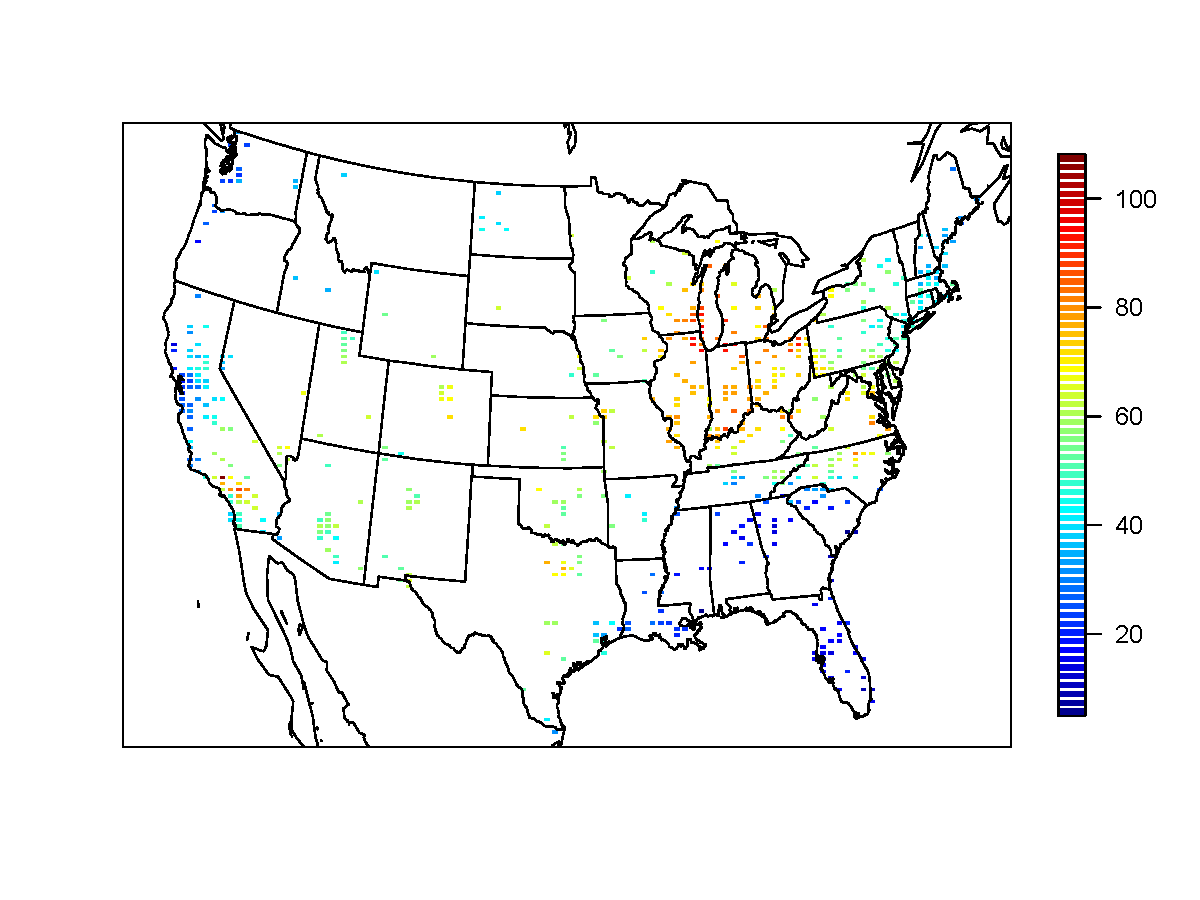
\includegraphics[width=\linewidth, trim=0 1in 0 1in ]{ozone-10jul-us}
%		\caption{Max 8-hour ozone measurements on July 10, 2005}
%		\end{figure}
% \end{frame}

% \begin{frame}{Defining extremes}
% 	\begin{columns}[c]
% 		\column{.45 \linewidth}
% 		\begin{itemize} \setlength{\itemsep}{1em}
% 			\item Key in extreme value analysis is to define extremes
% 			\item Typically done in one of two ways
% 			\begin{itemize}
% 				\item Block maxima (red dots)
% 				\item Values over threshold considered extreme
% 			\end{itemize}
% 		\end{itemize}

% 		\column{.55\linewidth}
% 		\begin{figure}
% 			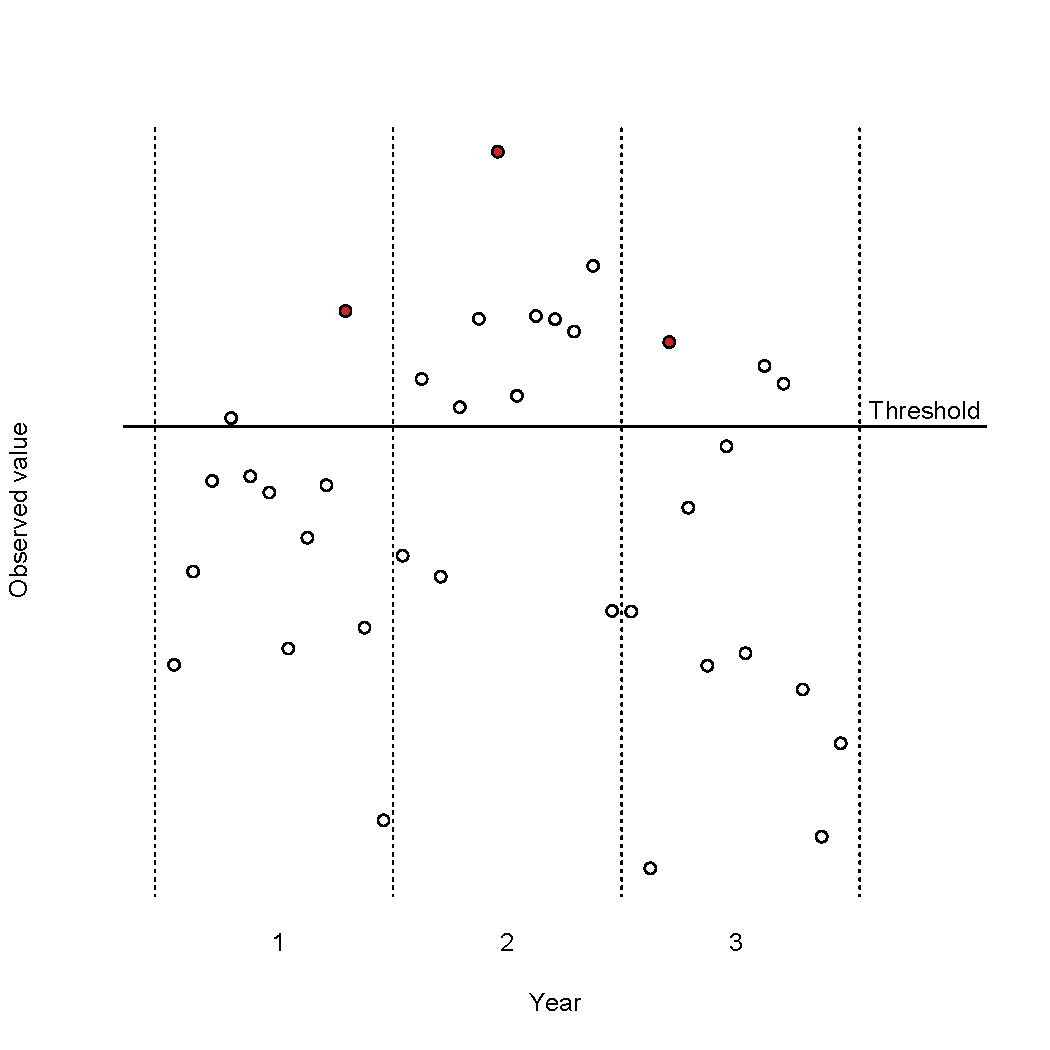
\includegraphics[width=1\linewidth, trim=0 0.5in 0 1in]{./plots/define_extreme.pdf}
% 			\caption{Hypothetical monthly data}
% 		\end{figure}
% 	\end{columns}
% \end{frame}

\begin{frame}{Non-spatial analysis: Block maxima}
	\begin{adjustwidth}{1em}{0em}
		Fisher-Tippett-Gnedenko theorem \vspace{1em}
		\begin{itemize} \setlength{\itemsep}{1em}
			\item Let $X_1, \ldots, X_t$ be i.i.d.
			\item Consider the block maximum $M_t = \max(X_1, \ldots, X_t)$
			\item If there exist normalizing sequences $a_t > 0$ and $b_t \in \calR$ such that $$\frac{ M_t - b_t }{ a_t } \converged G(z)$$ then $G(z)$ follows a generalized extreme value distribution (GEV) (Gnedenko, 1943)
			\item This motivates the use of the GEV for block maximum data
		\end{itemize}
	\end{adjustwidth}
\end{frame}

\begin{frame}{Non-spatial analysis: Block maxima}
	\begin{itemize} \setlength{\itemsep}{1em}
		\item GEV distribution
		\begin{align*}
			G(y) = \Pr(Y < y) = \begin{cases}
			\exp\left\{ -\left[ 1 + \xi \left( \frac{ y - \mu }{ \sigma } \right) \right]^{ -1 / \xi} \right\} & \quad \xi \neq 0 \\[0.5em]
			\exp \left\{ -\exp \left( - \frac{ y - \mu }{ \sigma} \right) \right\} & \quad \xi = 0
			\end{cases}
		\end{align*}
		where
		\begin{itemize} \setlength{\itemsep}{0.25em}
			\item $\mu \in \calR$ is a location parameter
			\item $\sigma > 0$ is a scale parameter
			\item $\xi \in \calR$ is a shape parameter
			\begin{itemize}
				\item Unbounded above if $\xi \ge 0$
				\item Bounded above by $(\mu - \sigma) / \xi$ when $\xi < 0$
			\end{itemize}
		\end{itemize}
		\item Challenges:
		\begin{itemize}
			\item Lose information by only considering maximum of a block
			\item Underlying data may not be i.i.d.
		\end{itemize}
	\end{itemize}
\end{frame}

\begin{frame}{Other approaches: Threshold methods}
	\begin{itemize} \setlength{\itemsep}{1em}
		\item Perhaps there exists a threshold $T$ beyond which values are extreme
		\item $T$ can be selected using a mean residual life plot.
		\item Two general approaches:
		\begin{itemize} \setlength{\itemsep}{0.5em}
			\item Peaks over threshold: Model $Y > T$ using generalized Pareto distribution
			\item Censored distribution function: $$F(y) = \begin{cases}
				F(T), & y \le T \\
				F(y), & y > T
			\end{cases}$$
		\end{itemize}
		\item Challenges: \vspace{0.5em}
		\begin{itemize} \setlength{\itemsep}{0.5em}
			\item Sensitive to threshold selection
			\item Temporal dependence
		\end{itemize}
	\end{itemize}
\end{frame}

% \begin{frame}{Non-spatial analysis: Peaks over threshold}
% \begin{adjustwidth}{1em}{0em}
%   Pickands-Balkema-de Haan theorem \vspace{1em}
%   \begin{itemize} \setlength{\itemsep}{1em}
%     \item Let $X_1, \ldots, X_n \iid F$
%     \item If there exist normalizing sequences $a_T > 0$ and $b_T \in \calR$ such that for any $x \ge 0$, as $T \rightarrow \infty$
%     \begin{align*}
%       \Pr\left(\frac{X - b_T}{a_T} > x \mid X > T\right) \converged H(x),
%     \end{align*}
%     where $T$ is a thresholding value, then $H(x)$ follows a generalized Pareto distribution (GPD) (Balkema and de Haan, 1974)
%   \end{itemize}
% \end{adjustwidth}
% \end{frame}

% \begin{frame}{Non-spatial analysis: Peaks over threshold}
% \begin{adjustwidth}{1em}{0em}
%   Select a threshold, $T$, and use the GPD to model the exceedances
%   \begin{align*}
%     H(y) = P(Y < y) = \left\{ \begin{array}{ll}
%       1 - \left[1 - \xi \left( \frac{ y - T }{ \sigma } \right) \right]^{-1 / \xi} & \quad \xi \neq 0 \\[0.5em]
%       1 - \exp \left\{ \frac{ y - T }{ \sigma} \right\} & \quad \xi = 0
%     \end{array}\right.
%   \end{align*}
%   where
%   \begin{itemize} \setlength{\itemsep}{0.25em}
%     \item $\sigma > 0$ is a scale parameter
%     \item $\xi \in \calR$ is a shape parameter
%     \begin{itemize}
%       \item Unbounded above if $\xi \ge 0$
%       \item Bounded above by $(T - \sigma) / \xi$ when $\xi < 0$
%     \end{itemize}
%   \end{itemize}
% \end{adjustwidth}
% \end{frame}

% \begin{frame}{Non-spatial analysis: Peaks over threshold}
%   \begin{itemize} \setlength{\itemsep}{1em}
%     \item The GPD is related to GEV distribution through
%     \begin{align*}
%       H(y) = 1 + \log[G(y)], \quad y \ge T
%     \end{align*}
%     \item Challenges: \vspace{0.5em}
%     \begin{itemize} \setlength{\itemsep}{0.5em}
%       \item Sensitive to threshold selection
%       \item Temporal dependence between observations (e.g. flood levels don't dissipate overnight)
%     \end{itemize}
%   \end{itemize}
% \end{frame}

\begin{frame}{Max-stable processes for spatial data}
	\begin{itemize} \setlength{\itemsep}{1em}
		\item Consider i.i.d. spatial processes $x_j(\bs)$, $j = 1, \ldots, t$
		\item Let $M_t(\bs) = \displaystyle\bigvee_{j=1}^t x_j(\bs)$ be the block maximum at site $\bs$
		\item If there exists normalizing sequences $a_t(\bs)$ and $b_t(\bs)$ such that for all sites, $\bs$,
		\begin{align*}
			\frac{M_t(\bs) - b_t(\bs)}{a_t(\bs)} \converged G(\bs)
		\end{align*}
		then $G(\bs)$ is a max-stable process (Smith, 1990)
		\item Therefore, max-stable processes are the standard model for block maxima
	\end{itemize}
\end{frame}

\begin{frame}{Multivariate representations}
	\begin{itemize} \setlength{\itemsep}{1em}
		\item Marginally at each site, observations follow a GEV distribution
		\item For a finite collection of $d$ sites the distribution function for the multivariate GEV (mGEV) is
		\begin{align*}
			\Pr(\bZ \le \bz)  &= G^*(\bz) = \exp[-V(\bz)]\\
			V(\bz)    &= d \int_{\Delta_d} \bigvee_{i = 1}^d \frac{w_i}{z_i} H(\ddd w)
		\end{align*}
		where
		\begin{itemize} \setlength{\itemsep}{0.25em}
			\item $V(\bz)$ is called the exponent measure (few closed-form expressions exist)
			\item $\Delta_d = \{ \bw \in \calR^d_+ \mid w_1 + \cdots + w_d = 1\}$
			\item $H$ is a probability measure on $\Delta_d$
			\item $\int_{\Delta_d}w_i H(\ddd w) = 1 / d$ for $i = 1, \ldots, d$
		\end{itemize}
	\end{itemize}
\end{frame}

% \begin{frame}{Multivariate GEV challenges}
% 	\begin{itemize} \setlength{\itemsep}{1em}
% 		\item Only a few closed-form expressions for $V(\bz)$ exist
% 		\item Two common forms for $V(\bz)$
% 		\begin{itemize}
% 			\item Symmetric logistic (Gumbel, 1960)
% 			\begin{align*}
% 				V(\bz) = \left[\sum_{i = 1}^n \left( \frac{ 1 }{ z_i } \right)^{1/\alpha}\right]^\alpha
% 			\end{align*}
% 			\item Asymmetric logistic (Coles and Tawn, 1991)
% 			\begin{align*}
% 				V(\bz) = \sum_{l = 1}^L \left[\sum_{i = 1}^n \left(\frac{w_{il}}{z_i} \right)^{1 / \alpha_l} \right]^{\alpha_l}
% 			\end{align*}
% 			where $w_{il} \in [0, 1]$ and $\sum_{l = 1}^L w_{il} = 1$
% 		\end{itemize}
% 	\end{itemize}
% \end{frame}

 %\begin{frame}{Multivariate peaks over threshold}
 %  \begin{itemize} \setlength{\itemsep}{1em}
 %    \item Few existing methods
 %    \item Often use max-stable methods due to the relationship between GEV and GPD
 %    \item Joint distribution function given by Falk et al. (2011)
 %    \begin{align*}
 %      H(\bz) = 1 - V(\bz)
 %    \end{align*}
 %    where $V(\bz)$ is defined as in the GEV
 %  \end{itemize}
 %\end{frame}

\begin{frame}{Quantifying dependence}
	\begin{itemize}\setlength{\itemsep}{1em}
		\item \alert{Problem}: Covariance and correlation focuses on deviations around the mean and not the extremes
		\item Want dependence measure to capture likelihood of seeing values that are jointly extreme
		\item Two common measures of dependence (bivariate):
		\begin{itemize}\setlength{\itemsep}{0.5em}
			\item Extremal coefficient $\vartheta \in (1, 2)$: $$P[Z(\bs_1)<c, Z(\bs_2)<c] = P[Z(\bs_1)<c]^{\vartheta(\bs_1,\bs_2)}$$
			\item $\chi \in (0, 1)$ (Coles, 1999): $$\chi(\bs_1,\bs_2) = \lim_{c\rightarrow \infty}P[Z(\bs_1)>c|Z(\bs_2)>c]$$
		\end{itemize}
	\end{itemize}
\end{frame}


\begin{frame}{Existing challenges}
	\begin{itemize} \setlength{\itemsep}{1em}
		\item Multivariate max-stable models have nice features, but they are
		\begin{itemize} \setlength{\itemsep}{0.5em}
			\item Computationally challenging (e.g,  the asymmetric logistic has $2^{n-1}(n + 2) - (2n + 1)$ free parameters)
			\item Joint density only available in low dimensions (Wadsworth and Tawn, 2014; Thibaud and Opitz, 2015)
		\end{itemize}
		\item Some recent approaches
		\begin{itemize} \setlength{\itemsep}{0.5em}
			\item Bayesian hierarchical model (Reich and Shaby, 2012)
			\item Pairwise likelihood (Padoan, 2010; Huser and Davison, 2014)
			\item Trivariate likelihood (Genton et al, 2011)
		\end{itemize}
		\item Many opportunities to explore new methods
	\end{itemize}
\end{frame}

\begin{frame}{Project 1: \Skewt{} for Threshold Exceedances}
	\begin{center}
		\LARGE
		\textbf{Project 1:}\\ [1em]
		A Space-time \Skewt{} Model for \\
		Threshold Exceedances\\ [2em]
		\normalsize
		Under revision: \\
		\emph{Biometrics}
	\end{center}
\end{frame}

\begin{frame}{Motivation}
	\begin{adjustwidth}{1em}{0em}
		Ozone compliance for Clean Air Act (EPA) \vspace{1em}
		\begin{itemize} \setlength{\itemsep}{1em}
			\item Annual fourth-highest daily maximum 8-hour concentration, averaged over 3 years, not to exceed 75 ppb
			\item Annual fourth-highest is the 99th percentile for the year
			\item Common objectives are \vspace{0.5em}
			\begin{itemize} \setlength{\itemsep}{0.5em}
				\item To interpolate to unmonitored sites
				\item Detect changes in extremes over time
				\item Study meteorological conditions that lead to extreme events
			\end{itemize}
		\end{itemize}
	\end{adjustwidth}
\end{frame}

\begin{frame}{Is max-stable the panacea?}
	\begin{itemize}\setlength{\itemsep}{1em}
		\item Max-stable process is an elegant approach, but does that mean it's correct? \vspace{0.5em}
		\begin{itemize} \setlength{\itemsep}{0.5em}
			\item It is only an approximation
			\item There are less complicated approximations (e.g. we could model daily data as a Gaussian process (GP))
		\end{itemize}
		\item If the goal is spatial interpolation, perhaps this is competitive
	\end{itemize}
\end{frame}


\begin{frame}{GP - Asymptotic Independence}
	\begin{itemize}\setlength\itemsep{1em}
		\item A GP leads to simple interpretation and computing, but asymptotic independence \vspace{0.5em}
		\begin{itemize} \setlength{\itemsep}{0.5em}
			\item If $Y(\bs_1)$ and $Y(\bs_2)$ are bivariate normal then $\chi(\bs_1,\bs_2)=0$ (asymptotic independence)
		\end{itemize}
		\item This suggests Kriging will not capture extremes
		\item So much is known for the Gaussian case: nonstationarity, multivariate, numerical approximations, \ldots
		\item Rather than toss it out, can we patch it up?
	\end{itemize}
\end{frame}


\begin{frame}{Spatial \skewt{} process}
A spatial \skewt{} process (Azzalini and Capitanio, 2014)  resembles a GP but exhibits asymptotic dependence
	\begin{eqnarray}
	 	Y_t(\bs) &=& \bX(\bs)^\top\bbeta +\lambda\sigma_t|z_t| + \sigma_tv_t(\bs)\nonumber\\
	 	z_t &\sim& \mbox{Normal}(0,1)\nonumber\\
	 	\sigma_t^2&\sim& \mbox{InvGamma}(a/2,b/2)\nonumber\\
	 	v_t&\sim& \mbox{Spatial GP}\nonumber
 	\end{eqnarray}
 	\begin{itemize}\setlength{\itemsep}{0.5em}
	 	\item Location: $\bX(\bs)^\top\bbeta$
	 	\item Scale: $b>0$
	 	\item Skewness: $\lambda\in{\cal R}$
	 	\item Degrees of freedom: $a>0$
	\end{itemize}
\end{frame}

\begin{frame}{Good properties}
 	\begin{itemize}\setlength{\itemsep}{1em}
 		\item Flexible $t$ marginal distribution with four parameters including the degrees of freedom which allows for heavy tails ($a=1$ gives a Cauchy)
 		\item Computation on the order of a GP; the only extra steps are $z_t$ and $\sigma_t$ which have conjugate full conditionals
 		\item Asymptotic dependence: $\chi(\bs_1,\bs_2)>0$ for all $\bs_1$ and $\bs_2$
 	\end{itemize}
\end{frame}

\begin{frame}{Bad properties and remedies}
	\begin{itemize}\setlength{\itemsep}{1em}
	 	\item Modeling all the data (bulk and extreme) can lead to poor tail probability estimates if the model is misspecified
	 	\item Long-range dependence: $\chi(\bs_1,\bs_2)>0$ for all $\bs_1$ and $\bs_2$ even if $\bs_1$ and $\bs_2$ are far apart
	 	\item This occurs because all sites share $z_t$ and $\sigma_t$
	 	\item Remedies: \vspace{0.5em}
	 	\begin{itemize}\setlength{\itemsep}{0.5em}
		 	\item We use a censored likelihood to focus on the tails
		 	\item We propose a local \skewt{} process
		 \end{itemize}
	\end{itemize}
\end{frame}

\begin{frame}{Censored likelihood}
	\begin{itemize}\setlength{\itemsep}{1em}
		\item Censored likelihood: We censor the data
		$${\tilde Y}_t(\bs) =\begin{cases}
			T 		 & \text{for } Y_t(\bs)\le T\\
		 	Y_t(\bs) & \text{for } Y_t(\bs)>T
		\end{cases}$$
		\item Censoring is handled using standard Bayesian imputation methods
		\item The threshold $T$ is chosen by cross-validation
		\item If $T$ is moderately extreme in the distribution (e.g. $q(0.75)$), set $\lambda = 0$
	\end{itemize}
\end{frame}

\begin{frame}{Local \skewt{} process}
	\begin{itemize}\setlength\itemsep{1em}
    \item Consider a set of spatial knots for day $t$
		\item Let the knots $\bv_{t1},...,\bv_{tK}$ follow a homogeneous Poisson process over the domain of interest (in practice we fix $K$)
		\item The knots partition the domain if we assign location $\bs$ to subregion $k=\argmin_{l}||\bs-\bv_{tl}||$
	\end{itemize}
\end{frame}

\begin{frame}{Local \skewt{} process}
	\begin{itemize}\setlength{\itemsep}{1em}
    \item Associated with each is \vspace{0.5em}
    \begin{itemize} \setlength{\itemsep}{0.5em}
      \item $z_{tk}\sim\mbox{Normal}(0,1)$
      \item $\sigma_{tk}^2\sim\mbox{InvGamma}(a/2,b/2)$
    \end{itemize}
		\item If $\bs$ is in subregion $k$ then $$Y_t(\bs) = \bX(\bs)^T\bbeta +\lambda\sigma_{tk}|z_{tk}| + \sigma_{tk}v_t(\bs)\nonumber$$
		\item The marginal distribution remains a $t$, but partitioning breaks long-range spatial dependence
	\end{itemize}
\end{frame}

 \begin{frame}{$\chi$-statistic by $h=||\bs_1-\bs_2||$}
 	\begin{center}
 		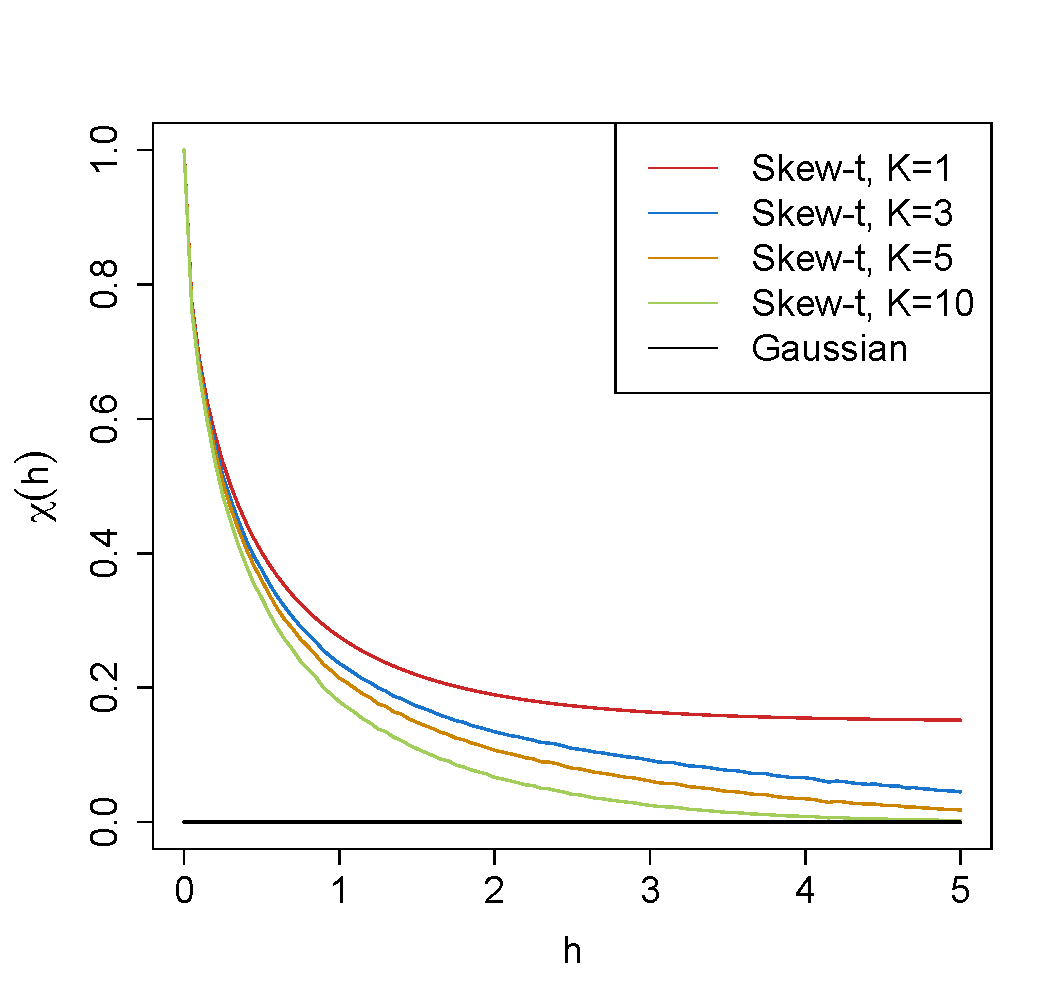
\includegraphics[height=0.8\textheight]{plots/chi-h}
 	\end{center}
 \end{frame}

 \begin{frame}{Temporal dependence}
 	\begin{itemize}\setlength\itemsep{1em}
 	\item It may not be reasonable to assume that observations are temporally independent (e.g. flooding, high temperatures)
 	\item Temporal dependence is handled through the $z_{tk}$, $\sigma_{tk}$ and $\bv_{tl}$
 	\item Method: \vspace{0.5em}
 	\begin{itemize}\setlength\itemsep{0.5em}
 	\item Use a copula to transform parameters to \emph{nice} space (i.e. $\mathcal{R}$)
 	\item AR(1) structure imposed on parameters in transformed space
 	\item Transform back to original parameter space to preserve \skewt{}
 	\end{itemize}
 	\end{itemize}
 \end{frame}


\begin{frame}{Results of a simulation study}
In terms of Brier scores for spatial prediction:\vspace{1em}
\begin{itemize}\setlength\itemsep{1em}
	\item Data generated as a GP:
	\begin{itemize}
	 	\item \skewt{} is close to GP
	 	\item max-stable is 15\% -- 30\% worse than GP
	\end{itemize}
	\item Data generated as a \skewt{} with multiple partitions:
	\begin{itemize}
		\item \skewt{} is 15\% better than GP
	 	\item max-stable is 30\% worse than GP
	\end{itemize}
	\item Data generated as asymmetric logistic (max-stable):
	\begin{itemize}
		\item \skewt{} is close to GP
		\item max-stable performs 10\% better than GP
	\end{itemize}
 	\item Data generated as Brown-Resnick (max-stable):
 	\begin{itemize}
		\item \skewt{} performs 40\% -- 60\% better than GP
 		\item max-stable performs 40\% -- 60\% better than GP
 	\end{itemize}
\end{itemize}
\end{frame}


 \begin{frame}{Application to ozone}
 	\begin{itemize}\setlength\itemsep{1em}
 	\item The USEPA has an extensive network of ozone monitors throughout the US
 	\item We will analyze ozone for 31 days in July, 2005 at $n=1,089$ stations
 	\item Currently the EPA regulates the annual 99$^{th}$ percentile
 	\item Our objective is to map the probability of an extreme ozone event
 	\end{itemize}
 \end{frame}

 \begin{frame}{Ozone on July 10}
 	\begin{center}
 		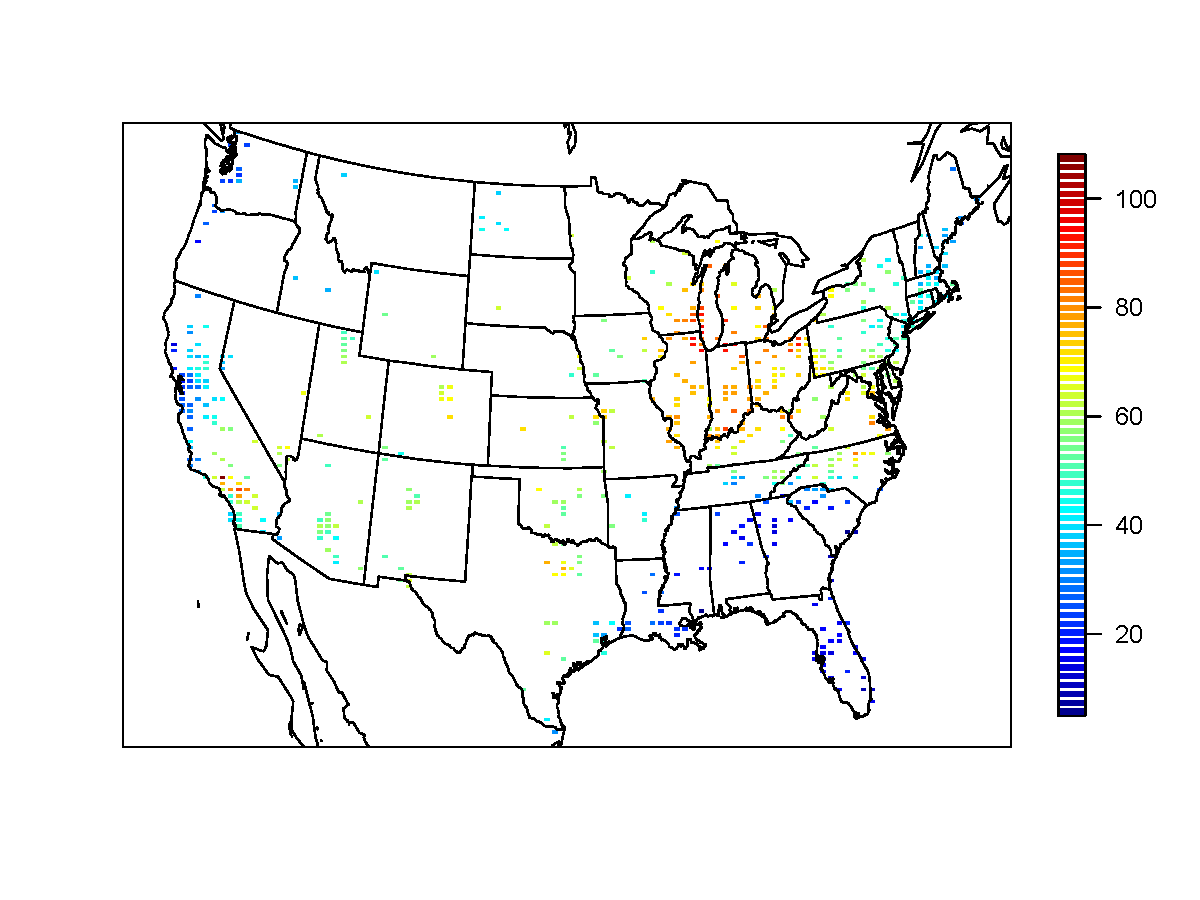
\includegraphics[width=1.2\textheight]{ozone-10jul-us}
 	\end{center}
 \end{frame}

 \begin{frame}{Q-Q plots}
 	\begin{center}
 		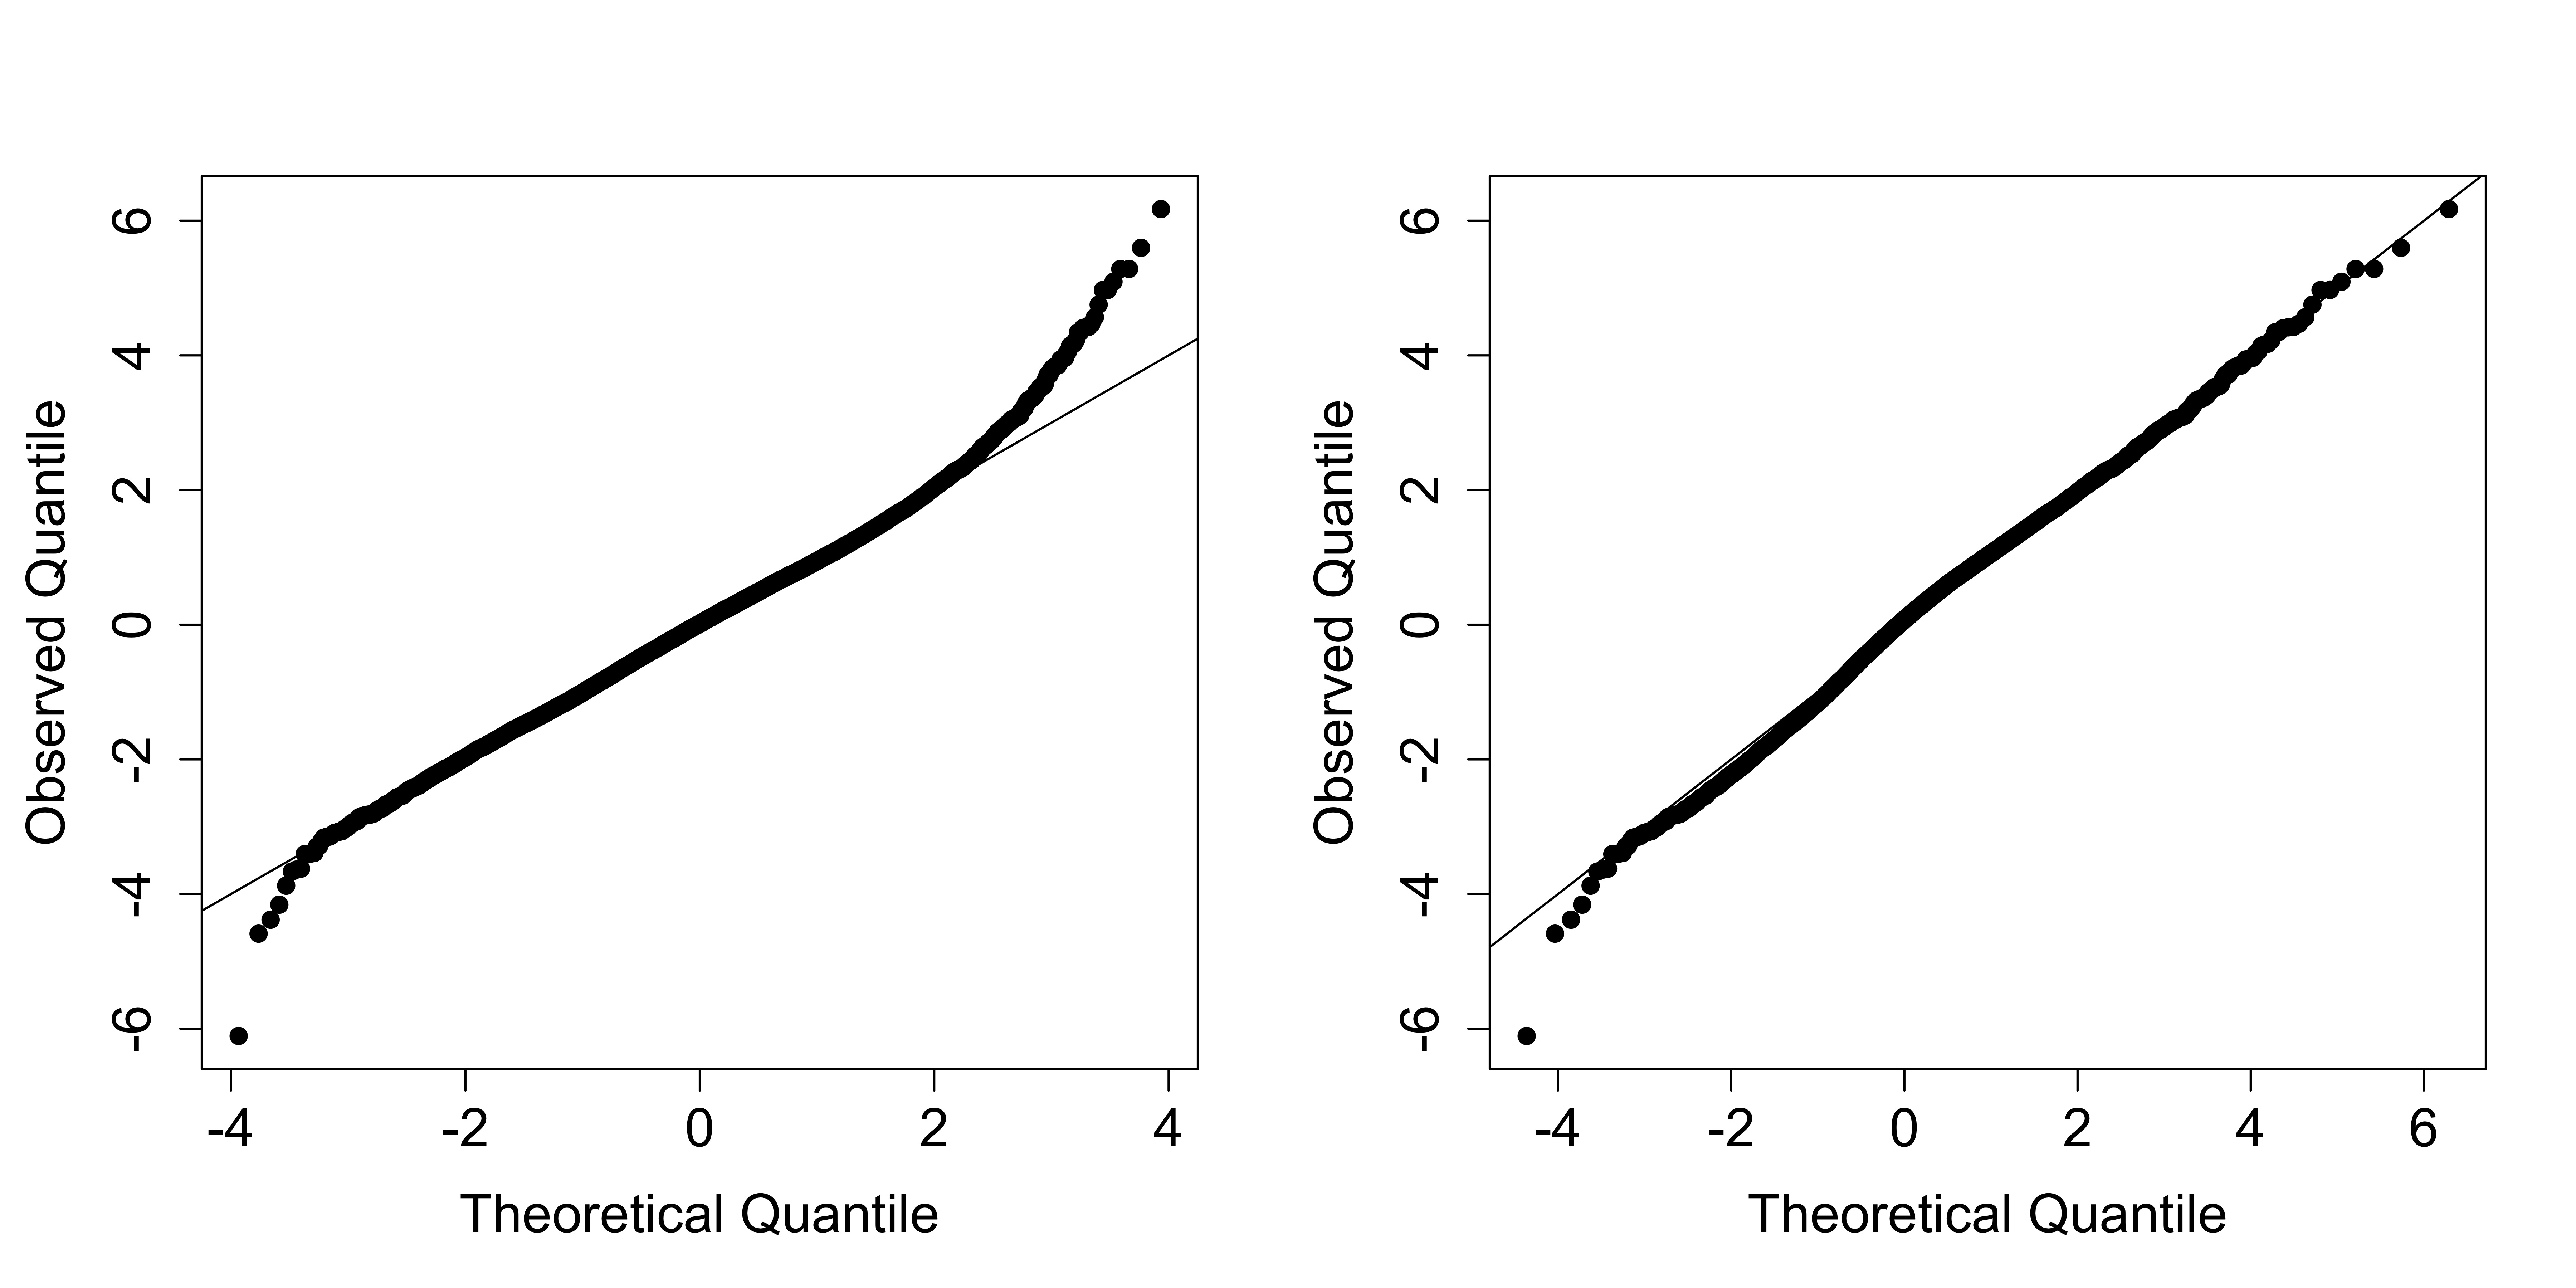
\includegraphics[width=0.9\textheight]{qq-res}

 		Gaussian Q-Q plot (left) and skew-$t$ with $a = 10$ and $\lambda = 1$ Q-Q plot (right)
 	\end{center}
 \end{frame}

 \begin{frame}{Cross-validation}
 	\begin{itemize}\setlength\itemsep{1em}
 	\item We split the sites into training and testing
 	\item We found that $K=15$ knots and censoring at $T$ equal to the median with no time series gave the best results
 	\item Results were not sensitive to these tuning parameters
 	\item This model was 5\% more accurate (Brier score) than GP
 	\item The max-stable model fit was 15\% less accurate than GP
 	\end{itemize}
 \end{frame}

 \begin{frame}{Fitted 99$^{th}$ percentiles}
 	\begin{center}
 		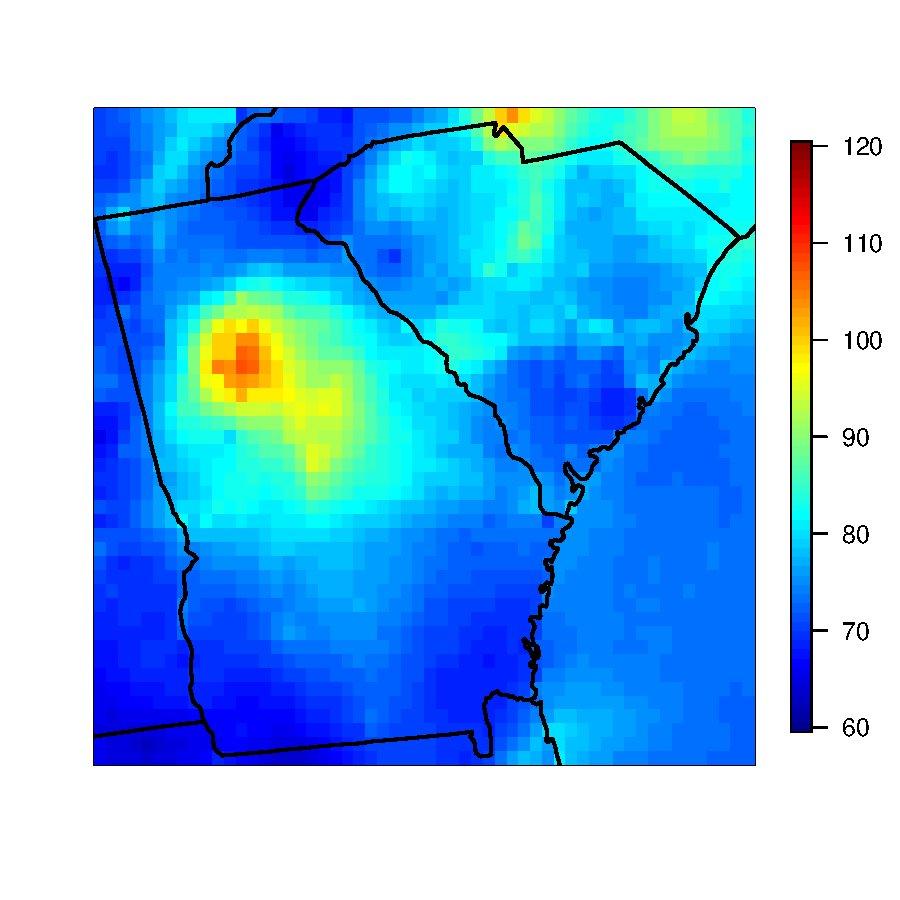
\includegraphics[width=0.45\linewidth]{q99gaus}
 		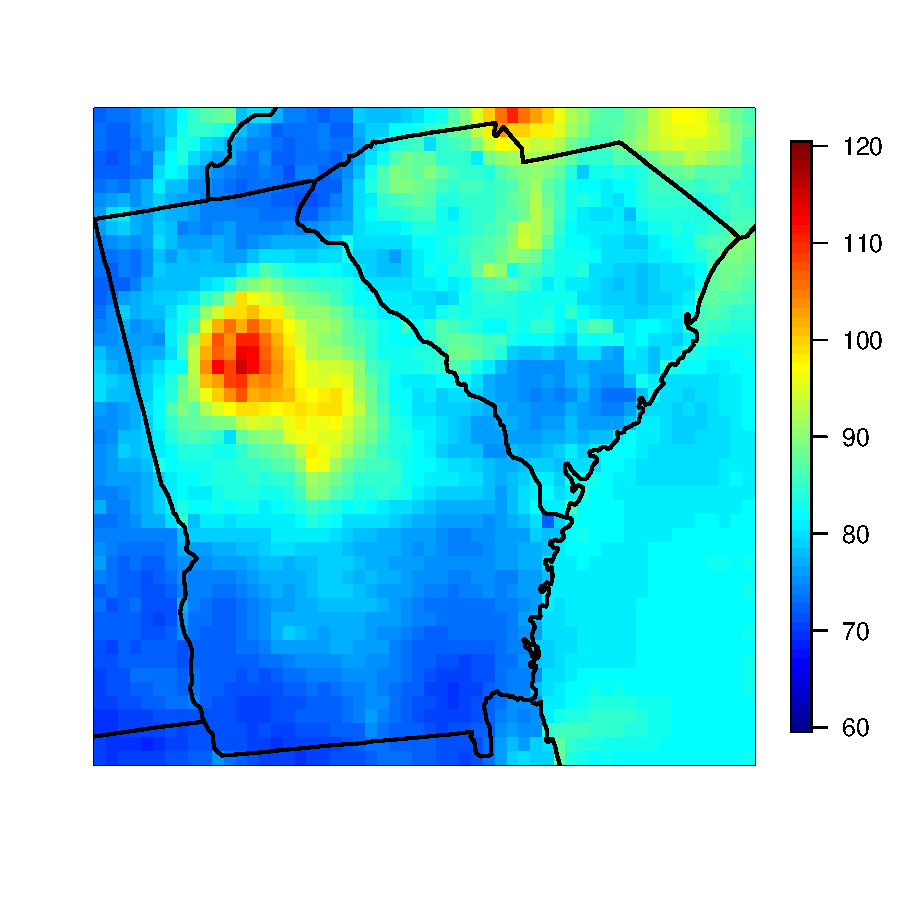
\includegraphics[width=0.45\linewidth]{q99skewtTS}

 		Gaussian (left) Symmetric-$t$, 10 knots, T = 75, Time series (right)
 	\end{center}
 \end{frame}

 \begin{frame}{Difference (Thresholded $t$ - Gaussian)}
 	\begin{center}
 		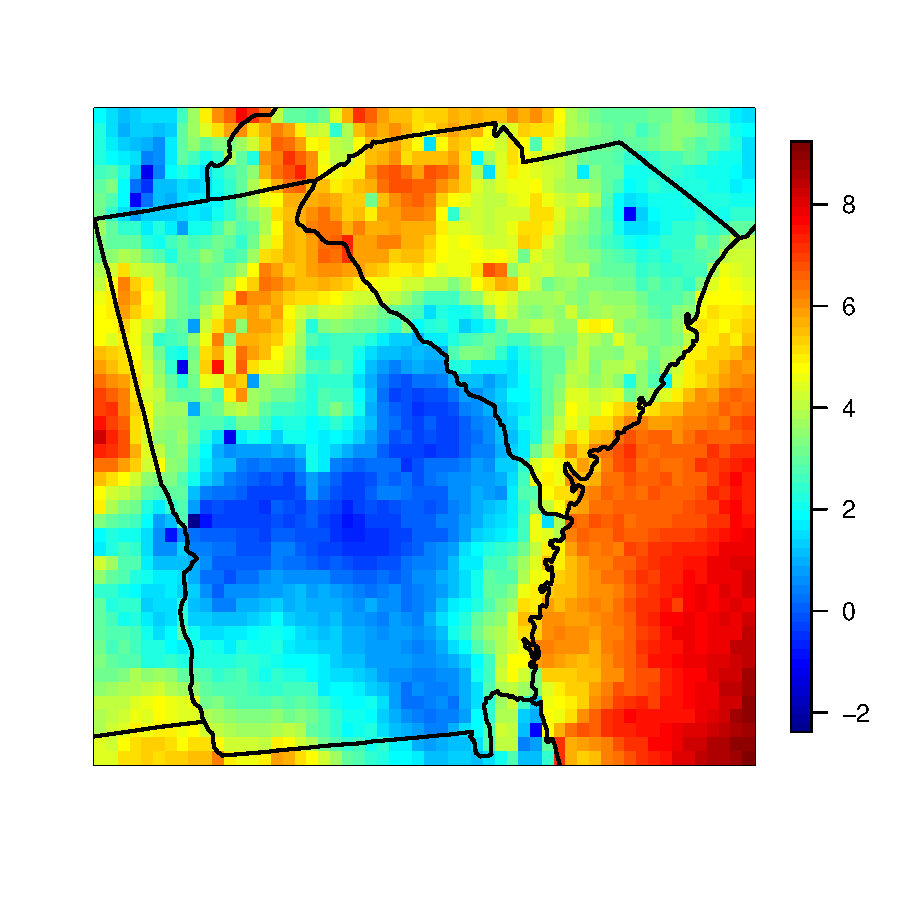
\includegraphics[width=0.45\linewidth]{q99diffgausskewt}

 		Difference between Symmetric-$t$, 10 knots, T = 75 and Gaussian
 	\end{center}
 \end{frame}

\begin{frame}{Project 2: Rare spatial binary}
	\begin{center}
		\LARGE
		\textbf{Project 2:}\\ [1em]
		Rare Spatial Binary Regression\\[2em]
		\normalsize
		To be submitted:\\
		\emph{Journal of Agricultural, Biological, and Environmental Statistics}
	\end{center}
\end{frame}

\begin{frame}{Motivation}
	\begin{center}
		\vspace{-3em}
		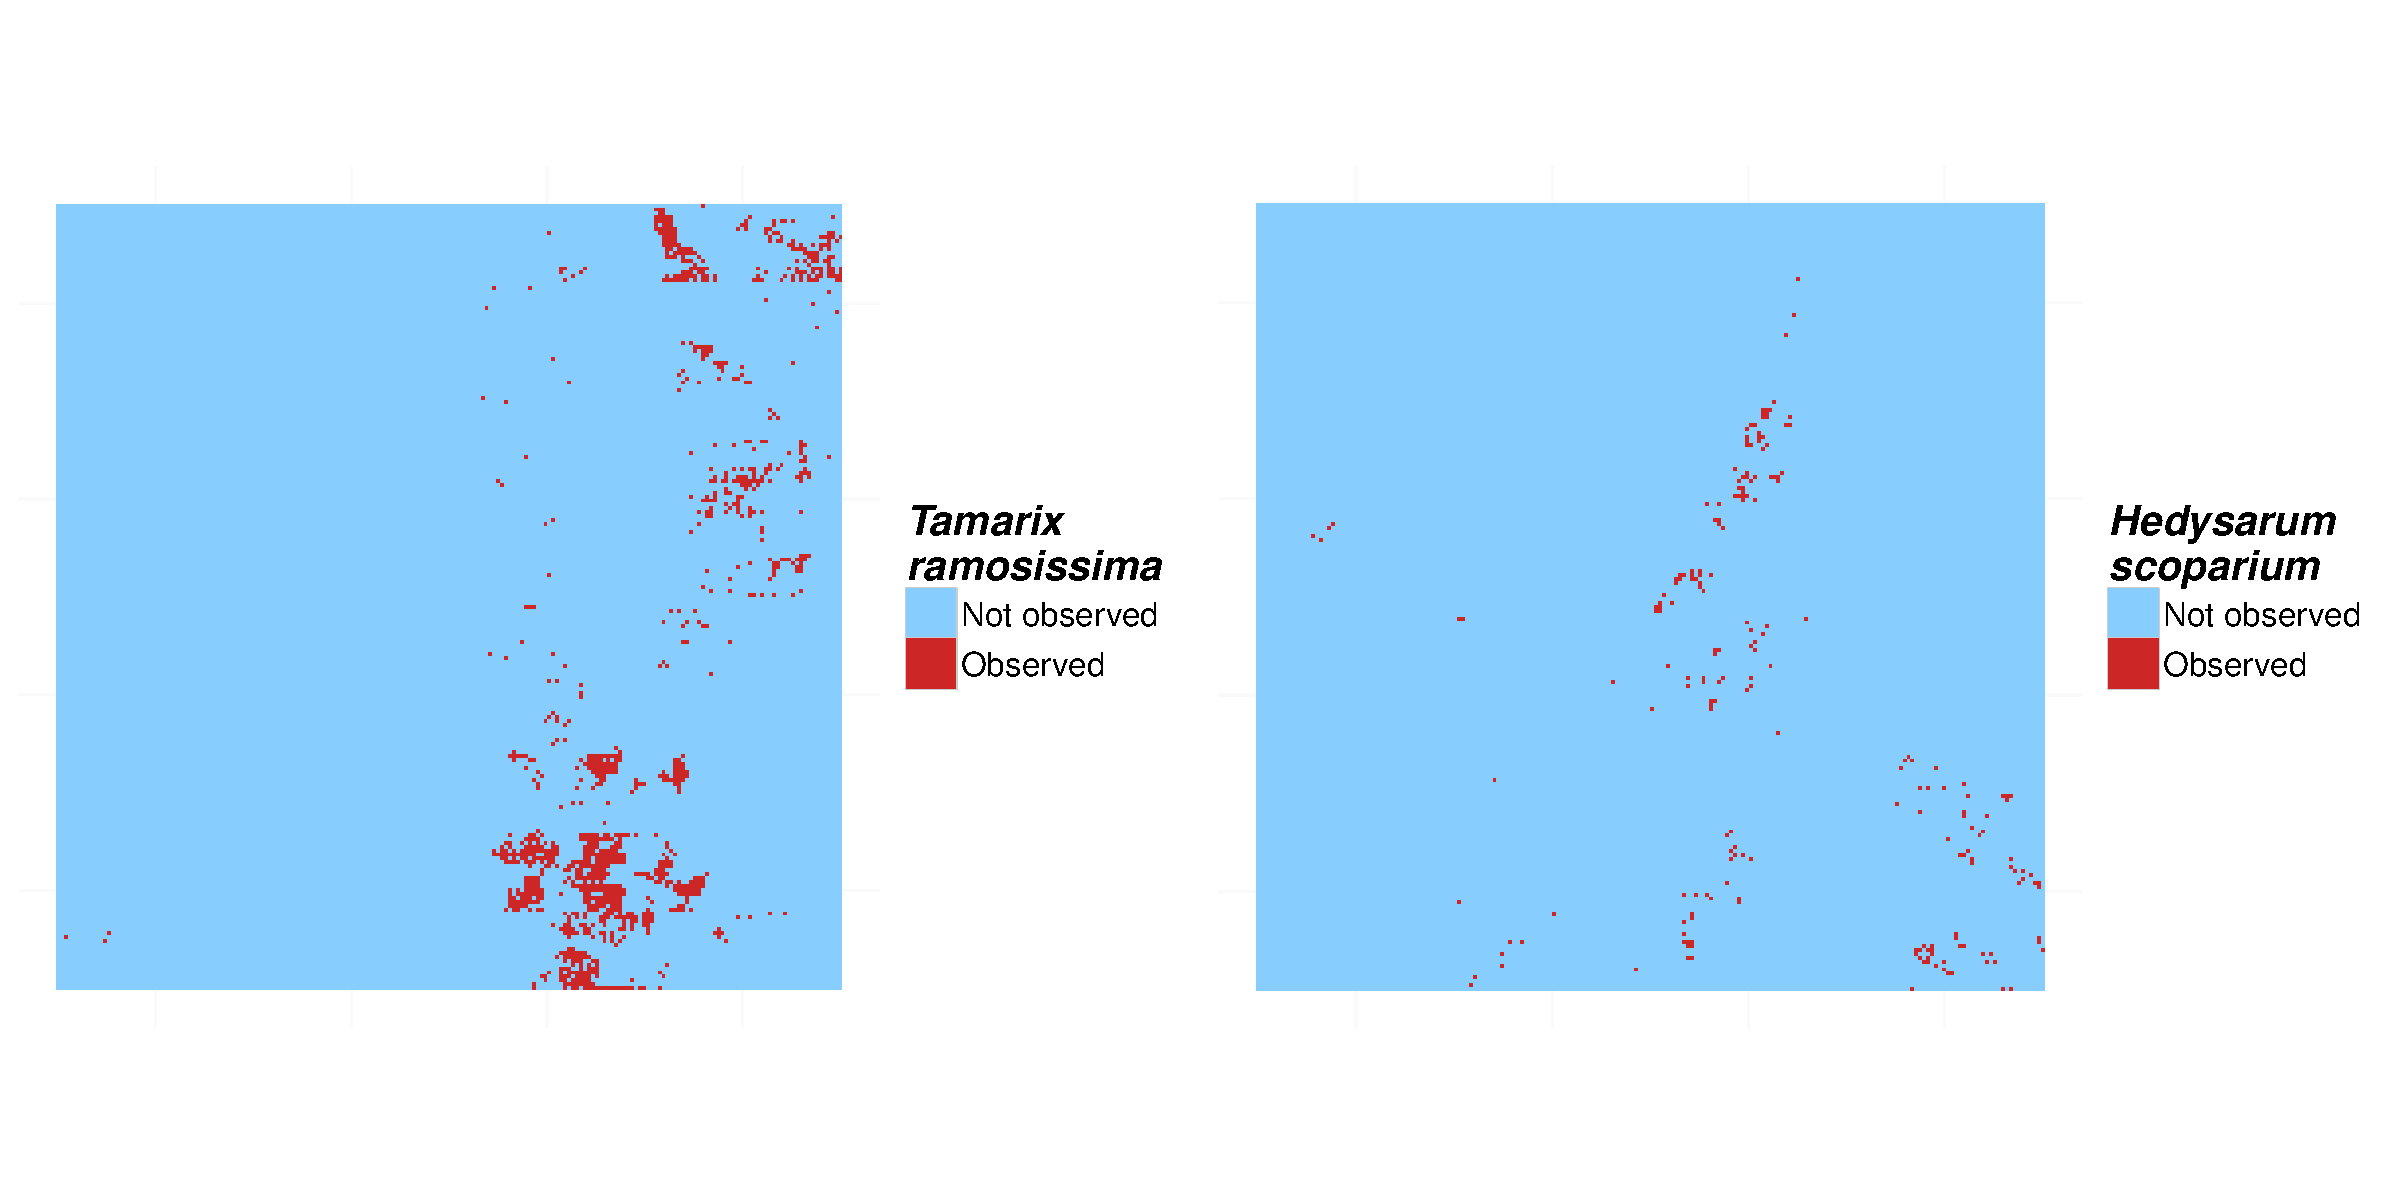
\includegraphics[width = 0.9\linewidth]{plant-census}
		\vspace{-1em}

		1-km$^2$ area in PR China.
	\end{center}
	\begin{itemize} \setlength{\itemsep}{0.5em}
		\item \tamarix{} (left) Rareness: $\approx 6\%$
		\item \hedysarum{} (right) Rareness: $\approx 0.5\%$
	\end{itemize}
\end{frame}

\begin{frame}{Motivation}
	\begin{itemize} \setlength{\itemsep}{1em}
		\item For rare species, occupancy modeling can be challenging \vspace{0.5em}
		\begin{itemize} \setlength{\itemsep}{0.5em}
			\item \alert{Rare}: to mean not occurring often (e.g. 5\% or less)
		\end{itemize}
		\item Binary regression is based on thresholding: $$Y(\bs) = I[Z(\bs) > c]$$
		\item GP traditionally used for $Z(\bs)$, but theory suggests that GP will not capture dependence  \vspace{0.5em}
		\begin{itemize} \setlength{\itemsep}{0.5em}
			\item $c$ is in the tail of the distribution
			\item Asymptotic dependence does not exist for GP
			\item Therefore for large $c$ this is virtually a non-spatial analysis
		\end{itemize}
		\item Propose max-stable extension to GEV link (Wang and Dey, 2010)
	\end{itemize}
\end{frame}

\begin{frame}{Hierarchical max-stable representation}
	\begin{itemize} \setlength{\itemsep}{1em}
    \item Representation from Reich and Shaby (2012)
		\item Consider a set of $L$ knots, $\bv_1, \ldots, \bv_L$
		\item Standardized Gaussian weights $w_l(\bs_i)$
		\begin{align*}
		w_l(\bs_i) = \frac{ \exp\left[ -0.5 \left( \frac{ || \bs_i - \bv_l || }{ \rho} \right)^2 \right]}{ \displaystyle \sum_{l = 1}^L \exp\left[ -0.5 \left( \frac{ || \bs_i - \bv_l || }{ \rho} \right)^2 \right] }
		\end{align*}
		\item Is a valid a low-rank approximation if $L < n$, but in this application we place knots at all data points
	\end{itemize}
\end{frame}

\begin{frame}{Hierarchical max-stable representation}
	\begin{itemize} \setlength{\itemsep}{1em}
		\item Model the spatial dependence using
		\begin{align*}
		\theta(\bs) = \left[\sum_{l = 1}^L A_l w_l(\bs)^{1 / \alpha}\right]^\alpha
		\end{align*}
		where
		\begin{itemize} \setlength{\itemsep}{0.5em}
			\item $A_l \iid \text{PS}(\alpha)$ are positive stable random effects
			\item $w_l(\bs)$ are scaled kernel function so that $\sum_{l = 1}^L w_l(\bs) = 1$
			\item $\alpha \in (0, 1)$ is a parameter controlling strength of spatial dependence in residuals (0: high, 1: independent)
		\end{itemize}
	\end{itemize}
\end{frame}

\begin{frame}{Hierarchical max-stable representation}
	\begin{itemize} \setlength{\itemsep}{1em}
		\item Let $Z(\bs)$ be a max-stable process
		\item Conditioned on the random effects $A_1, \ldots, A_L$, then
		\begin{align*}
		Z(\bs_i) \mid A_l &\ind \text{GEV}[\mu^*(\bs_i), \sigma^*(\bs_i), \xi^*] \\
		A_l &\iid \text{PS}(\alpha)
		\end{align*}
		where
		\begin{align*}
			\mu^*(\bs_i) &= \bX(\bs_i)^\top \bbeta +  \frac{\theta(\bs_i)^{\xi} - 1}{\xi}\\
			\sigma^*(\bs_i) &= \alpha \theta(\bs_i)^{\xi}\\
			\xi^* &= \alpha \xi
		\end{align*}
		\item The marginal distribution at site $\bs_i$ is GEV$[\bX(\bs_i)^\top \bbeta, 1, \xi]$
	\end{itemize}
\end{frame}

\begin{frame}{Hierarchical model}
	\begin{itemize} \setlength{\itemsep}{1em}
		\item Hierarchical model:
		\begin{align*}
		Y(\bs_i) | A_l &\ind \text{Bern}\{\pi(\bs_i)\}\\
		\pi(\bs_i) &= 1 - \exp\left\{ \sum_{l = 1}^L A_l \left[\frac{ w_l (\bs_i) }{z(\bs_i)} \right]^{1 / \alpha} \right\}\\
		\end{align*} \vspace{-0.5em}
		where $$z(\bs_i) = \begin{cases}
		(1 - \xi \bX(\bs_i) \bbeta)^{-1 / \xi} & \xi \neq 0 \\
		\exp(-\bX(\bs_i) \bbeta) & \xi = 0
		\end{cases}$$
    \item Fix $\xi = 0$ when no covariates
	\end{itemize}
\end{frame}

\begin{frame}{Spatial dependence}
	\begin{itemize} \setlength{\itemsep}{1em}
		\item Cohen's kappa: $$\kappa(\beta) = \frac{P_A - P_E}{1 - P_E}$$
		where
		\begin{itemize} \setlength{\itemsep}{0.5em}
			\item $P_A$: Joint probability of agreement
			\item $P_E$: Joint probability of agreement under assumption of independence
		\end{itemize}
		\item Consider $Z(\bs_1)$ and $Z(\bs_2)$ both GEV$(\beta, 1, 1)$ then $$\kappa = \lim_{\beta \rightarrow \infty} \kappa(\beta) = 2 - \vartheta(\bs_1, \bs_2) = \chi$$
		\item When $Z(\bs)$ is Gaussian, $\kappa = 0$
	\end{itemize}
\end{frame}


\begin{frame}{Simulation study: Settings}
	\begin{itemize} \setlength{\itemsep}{1em}
		\item 50 simulated populations: \vspace{0.5em}
		\begin{itemize} \setlength{\itemsep}{0.5em}
			\item Link: GEV, Logistic, Hotspot
			\item Data generated on $100 \times 100$ grid
		\end{itemize}
		\item Sample datasets:
  \end{itemize}
	\begin{center}
		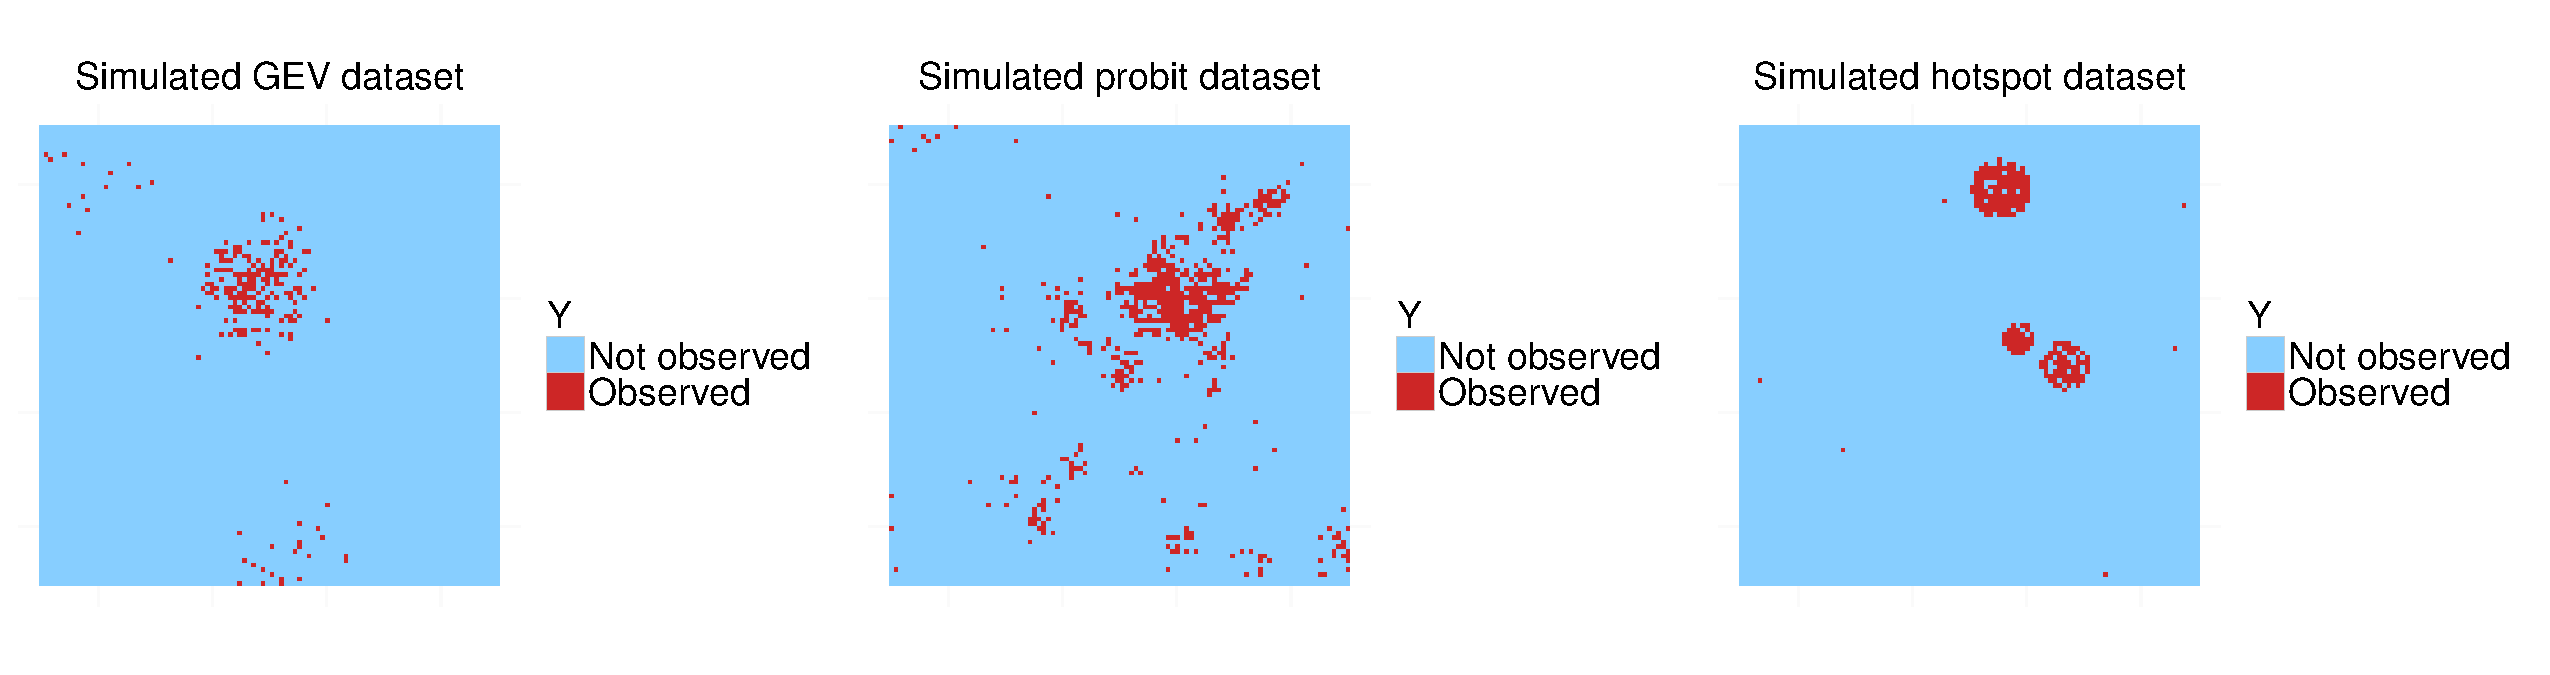
\includegraphics[width=\linewidth]{simulateddata.pdf}
	\end{center}
\end{frame}

\begin{frame}{Simulation study: Settings}
	\begin{itemize} \setlength{\itemsep}{1em}
		\item Sampling strategies: \vspace{0.5em}
		\begin{itemize} \setlength{\itemsep}{0.5em}
			\item Sample type: Cluster, Simple Random Sample
			\item Sample size: $n = 100$, $250$ initial sites
		\end{itemize}
		\item Models fit: \vspace{0.5em}
		\begin{itemize} \setlength{\itemsep}{0.5em}
			\item Spatial GEV ($\xi = 0$)
			\item Spatial probit
			\item Spatial logistic (\texttt{spBayes::spGLM})
		\end{itemize}
		\item Consider Brier score and area under receiver operating characteristic (AUROC) curve
	\end{itemize}
\end{frame}


\begin{frame}{Simulation study: Results}
	\begin{itemize} \setlength{\itemsep}{1em}
		\item Results: \vspace{0.5em}
		\begin{itemize} \setlength{\itemsep}{0.5em}
			\item GEV model shows small advantage over others for GEV link with $n = 250$ and cluster sampling
			\item Probit wins in other settings, but GEV is similar
		\end{itemize}
		\item Results provide some evidence of advantage for GEV method as rareness increases
	\end{itemize}
\end{frame}

\begin{frame}{Simulation study: Results}
	\begin{center}
		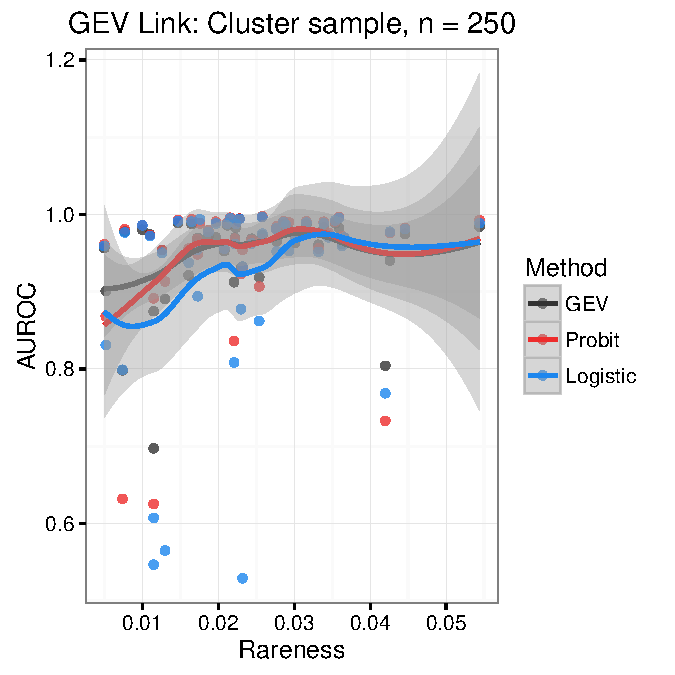
\includegraphics[width=0.49\linewidth]{byrareness-3}
    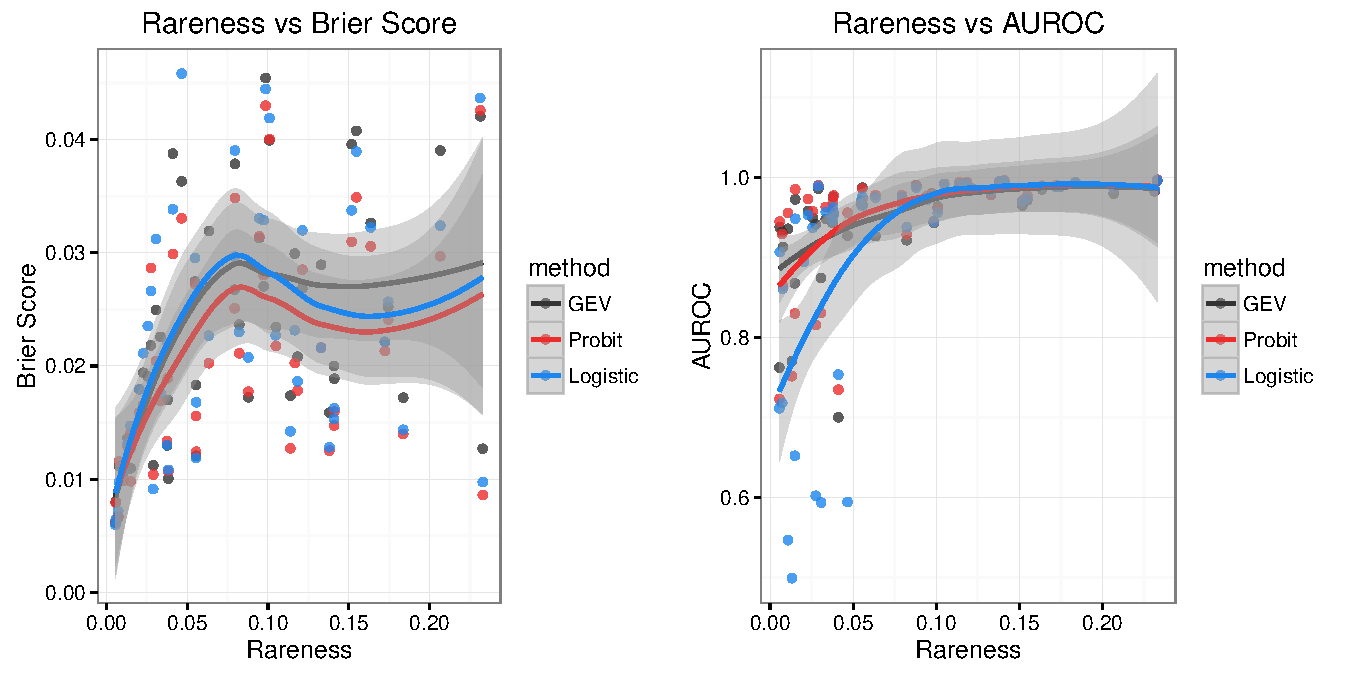
\includegraphics[width=0.49\linewidth]{byrareness-4}

		Loess smooth of AUROC by rareness for GEV link functions
	\end{center}
\end{frame}

\begin{frame}{Simulation study: Results}
  \begin{center}
    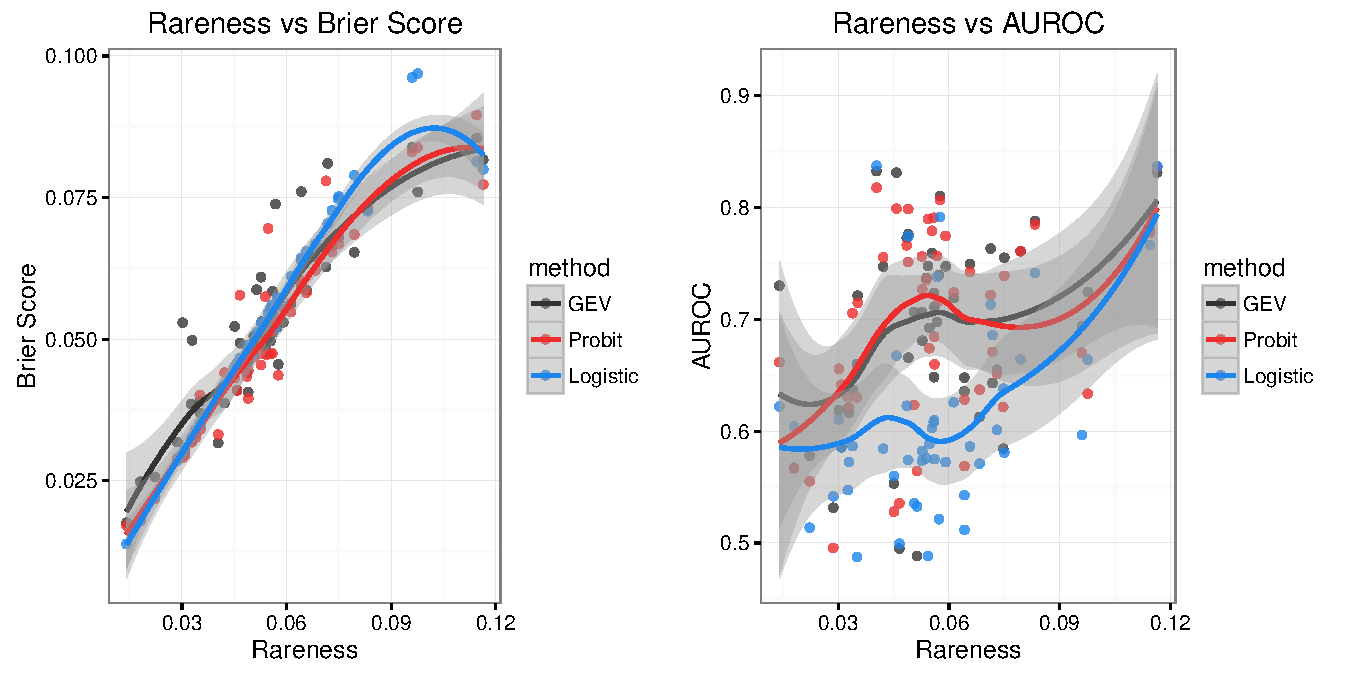
\includegraphics[width=0.49\linewidth]{byrareness-6}
    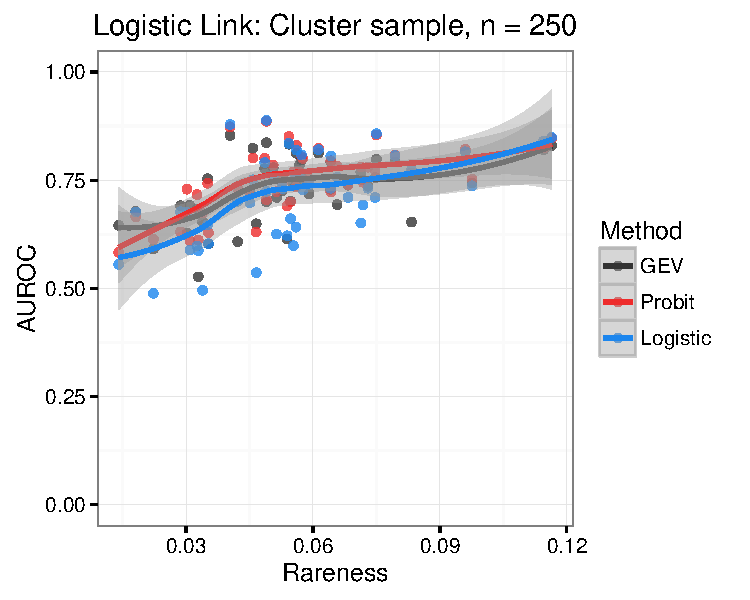
\includegraphics[width=0.49\linewidth]{byrareness-7}

    Loess smooth of AUROC by rareness for logistic link functions
  \end{center}
\end{frame}

\begin{frame}{Data analysis}
	\begin{itemize}\setlength{\itemsep}{1em}
		\item Census data for \tamarix{} ($\approx 6\%$) and \hedysarum{} ($\approx 0.5\%$) in 1-km$^2$ region of PR China
		\item Analysis similar to simulation study
		\begin{itemize} \setlength{\itemsep}{0.5em}
			\item Sample types: Cluster, Simple Random Sample
			\item Sample sizes: $n = 100$, $250$ initial sites
			\item Models fit: Spatial GEV ($\xi = 0$), probit, logit
		\end{itemize}
		\item 50 samples taken from each species for each sample type and sample size
	\end{itemize}
\end{frame}

\begin{frame}{Data analysis: Results}
	\begin{itemize} \setlength{\itemsep}{1em}
		\item Support simulation finding about GEV performance with respect to rareness
		\item For \tamarix{}, probit generally performs better
		\item For \hedysarum{}, with cluster sampling and for smaller sample sizes, GEV model generally performs better
	\end{itemize}
\end{frame}

\begin{frame}{Data analysis: Results}
	\begin{center}
		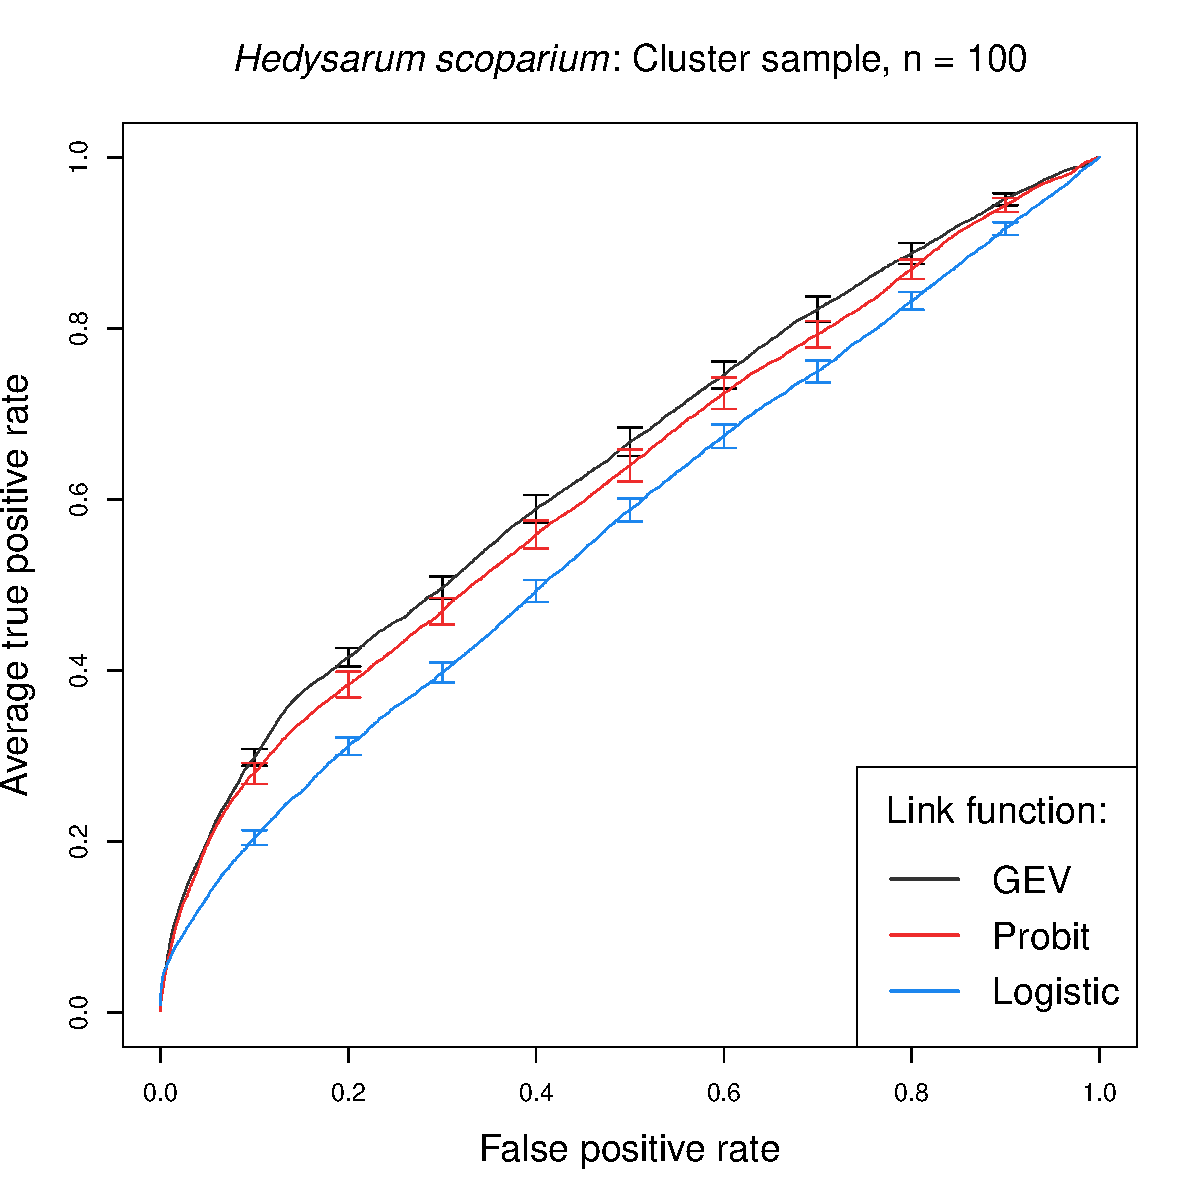
\includegraphics[width=0.47\textwidth]{data-perf-species2-100-clu}
		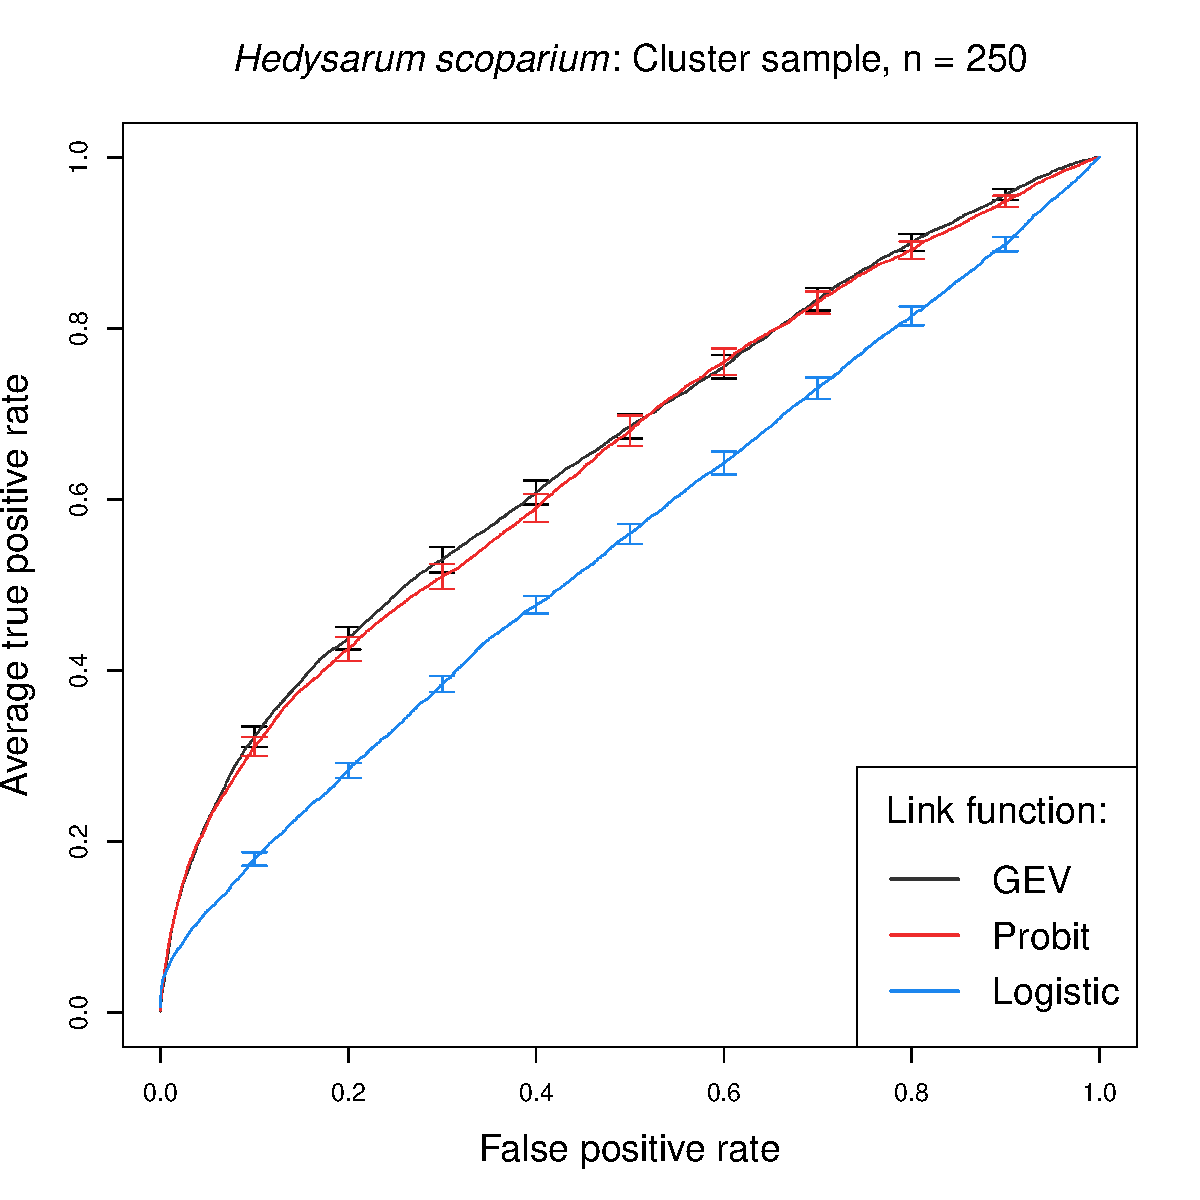
\includegraphics[width=0.47\textwidth]{data-perf-species2-250-clu}

		ROC curves for \hedysarum{}
	\end{center}
\end{frame}

\begin{frame}{Project 3: Empirical Basis Functions}
	\begin{center}
		\LARGE
		\textbf{Project 3:}\\ [1em]
		Empirical Basis Functions for \\
		Max-stable Dependence\\ [2em]
		\normalsize
		To be submitted:\\
		\emph{Annals of Applied Statistics}
	\end{center}
\end{frame}

\begin{frame}{Motivation}
	\begin{itemize} \setlength{\itemsep}{1em}
		\item Want fit max-stable models on high dimensional data
		\item When $n$ is large, computing is onerous
		\item Dimension reduction by placing $L < n$ spatial knots and using standardized Gaussian kernel functions as in Reich and Shaby (2012) and Project 2
		\item This works, but can we improve performance with a different set of basis functions \vspace{0.5em}
		\begin{itemize} \setlength{\itemsep}{0.5em}
			\item Exploratory data analysis like principal components (PC)
			\item Useful for inference and predictions
		\end{itemize}
	\end{itemize}
\end{frame}

\begin{frame}{Low-rank positive-stable representation}
	\begin{itemize} \setlength{\itemsep}{1em}
		\item Any max-stable process can be written as pointwise maximum of infinitely many processes (deHaan, 2006)
		\item Wang and Stoev (2011) truncate at $L$ processes
		\item Unlikely that a realization is equal to the point-wise maximum of $L$ processes, so we follow Reich and Shaby (2012) and set $$Z_t(\bs) = \theta_t(\bs) \varepsilon_t(\bs)$$ where $\theta_t(\bs)$ is a spatial process and $\varepsilon_t(\bs) \iid$ GEV$(1, \alpha, \alpha)$
	\end{itemize}
\end{frame}

\begin{frame}{Low-rank positive-stable representation}
	\begin{itemize}\setlength{\itemsep}{1em}
    \item Spatial process is $$\theta_t(\bs) = \left( \sum_{l = 1}^L A_{tl} B_l(\bs)^{1 / \alpha} \right)^\alpha$$ where $A_{tl} \sim$ PS$(\alpha)$
		\item $Z_t$ is max-stable marginally over the random effects $A_{tl}$
		\item The joint distribution is mGEV with asymmetric logistic dependence function
	\end{itemize}
\end{frame}

\begin{frame}{Low-rank positive-stable representation}
  \begin{itemize}\setlength{\itemsep}{1em}
    \item Dependence is measured by the extremal coefficient $\vartheta$, defined via $$P[Z_t(\bs_1)<c, Z_t(\bs_2)<c] = P[Z_t(\bs_1)<c]^{\vartheta(\bs_1,\bs_2)}$$
    \item For the low-rank PS model $$\vartheta(\bs_1,\bs_2) = \sum_{l=1}^L\left[B_l(\bs_1)^{1/\alpha}+B_l(\bs_2)^{1/\alpha}\right]^{\alpha}\in[1,2] $$
    \item Propose to use empirical basis functions for $B_l(\bs)$ (instead of $w_l(\bs)$ from rare binary)
  \end{itemize}
\end{frame}

\begin{frame}{Estimating the EBFs, $B_l(\bs)$}
	\begin{enumerate}[1.]\setlength\itemsep{1em}
		\item Use a rank transformation to standardize data for each $\bs$
		\item Estimate the extremal dependence between each pair of sites (using $\chi$ or madogram), ${\hat \vartheta}(\bs_i,\bs_j)$
		\item Spatially (4D) smooth the sample dependence measures for $\tilde{\vartheta}(\bs_i, \bs_j)$
		\item Constrained least squares (next slide) to minimize the distance between sample ($\tilde{\vartheta}$) and model ($\vartheta$ as a function of the $B$) spatial dependence
		\item Order the terms by $v_l = \sum_{\bs}B_l(\bs)$
	\end{enumerate}
\end{frame}


\begin{frame}{Estimating the EBFs, $B_l(\bs)$}
	\begin{itemize}\setlength\itemsep{1em}
		\item The objective function to estimate the $B_l$ is
		$$ \sum_{i<j}\left[\tilde{\vartheta}(\bs_i,\bs_j) - \vartheta(\bs_i,\bs_j)\right]^2$$
		where $\vartheta(\bs_i,\bs_j)$ is a function of $B_l$
		\item The EBFs must satisfy $B_l(\bs)>0$ and $\sum_{l}B_l(\bs)=1$ for all $\bs$
		\item The solution is approximated by cycling through the sites and solving a series of constrained optimization problems
    \item Also gives estimate of $\hat{\alpha}$
	\end{itemize}
\end{frame}

\begin{frame}{Comparison with PCA}
	\begin{itemize} \setlength{\itemsep}{1em}
		\item Similarities to PCA: \vspace{0.5em}
		\begin{itemize} \setlength{\itemsep}{0.5em}
			\item Reduces dimension
			\item Maps of $B_l(\bs)$ tell us about the most important spatial patterns
			\item Captures a non-stationary spatial dependence structure
		\end{itemize}
		\item Differences from PCA: \vspace{0.5em}
		\begin{itemize} \setlength{\itemsep}{0.5em}
			\item Basis functions are not orthonormal
			\item Loadings are positive stable, not Gaussian
			\item Loadings $A_{lt}$ may not be independent
			\item Computing $A$ and $B$ is not as simple as a few matrix operations
		\end{itemize}
	\end{itemize}
\end{frame}

%\begin{frame}{Contrasts with PCA}
%	\begin{itemize}\setlength{\itemsep}{1em}
%		\item Basis functions are not orthonormal
%		\item Loadings are positive stable, not Gaussian
%		\item Loadings $A_{lt}$ may not be independent
%		\item Computing $A$ and $B$ is not as simple as a few matrix operations
%	\end{itemize}
%\end{frame}
%
%\begin{frame}{Analogy with PCA}
%	\begin{itemize}\setlength{\itemsep}{1em}
%		\item Reduces the dimension from $n$ to $L$
%		\item Maps of $B_l(\bs)$ tell us about the most important spatial patterns
%		\item Captures a non-stationary spatial dependence structure
%		\item The $v_l$ tell us how many important features are present
%		\item Loadings $A_{lt}$ can be estimated and fed into future analyses
%	\end{itemize}
%\end{frame}


\begin{frame}{Bayesian implementation}
	\begin{itemize}\setlength{\itemsep}{1em}
		\item Given the basis function $B_l(\bs)$ and $\hat{\alpha}$ we can proceed with MCMC to estimate the remaining parameters
		\begin{align*}
		  \mu_t(\bs) &= \beta_{1,int}(\bs) + \beta_{1,time}(\bs)t\\
		  \log[\sigma_t(\bs)] &= \beta_{2,int}(\bs) + \beta_{2,time}(\bs)t\\
		  \xi_t(\bs) &= \xi
		\end{align*}
		\item Gaussian process priors on $\beta(\bs)$ terms
		\item We use cross-validation (quantile and Bries scores) to select $L$
		\item Alternative: select $L$ so that $\sum_{l=1}^Lv_l = 0.8$
	\end{itemize}
\end{frame}


\begin{frame}{Application 1: Wildfires in GA}
	\begin{itemize}\setlength{\itemsep}{1em}
		\item The data are the number of acres burned by forest fires (wildfire) each year (1965--2014) in each county of Georgia
		\item We censor the data at the local 95$^{th}$ percentile, $T(\bs)$
		\item The objectives are to map fire risk and determine if it is changing with time
	\end{itemize}
\end{frame}


\begin{frame}{Fire: Time series for each county }
	\begin{center}
		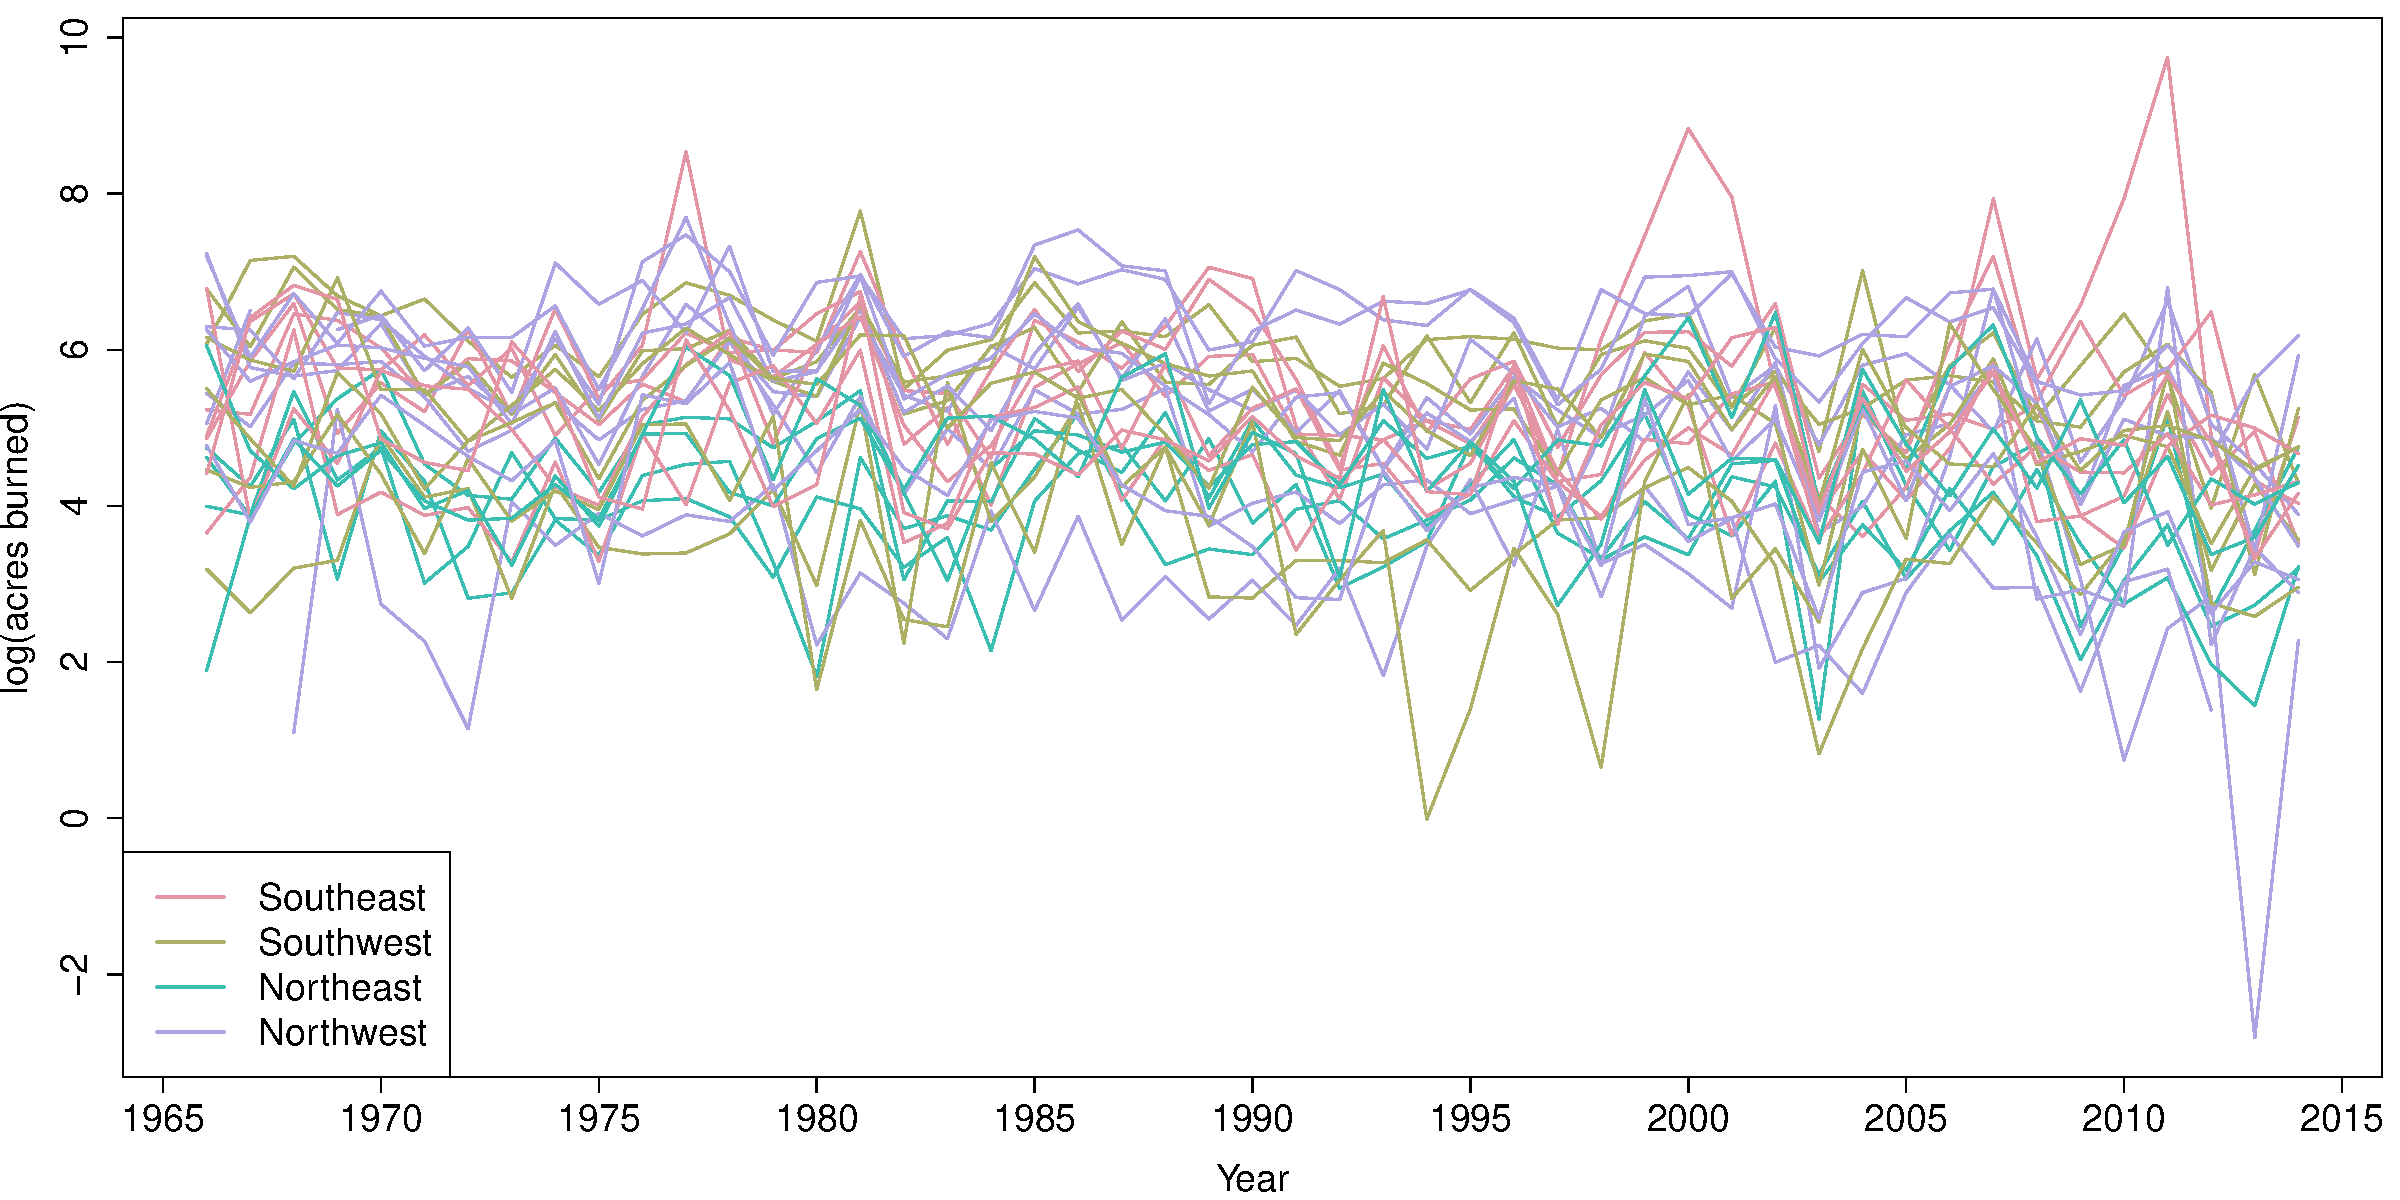
\includegraphics[width=0.8\textwidth]{fire-spag-rand-25}

    Time series of $\log(\text{acres burned})$ color-coded by region.
	\end{center}
\end{frame}


\begin{frame}{Fire: Picking the threshold}
	\begin{center}
		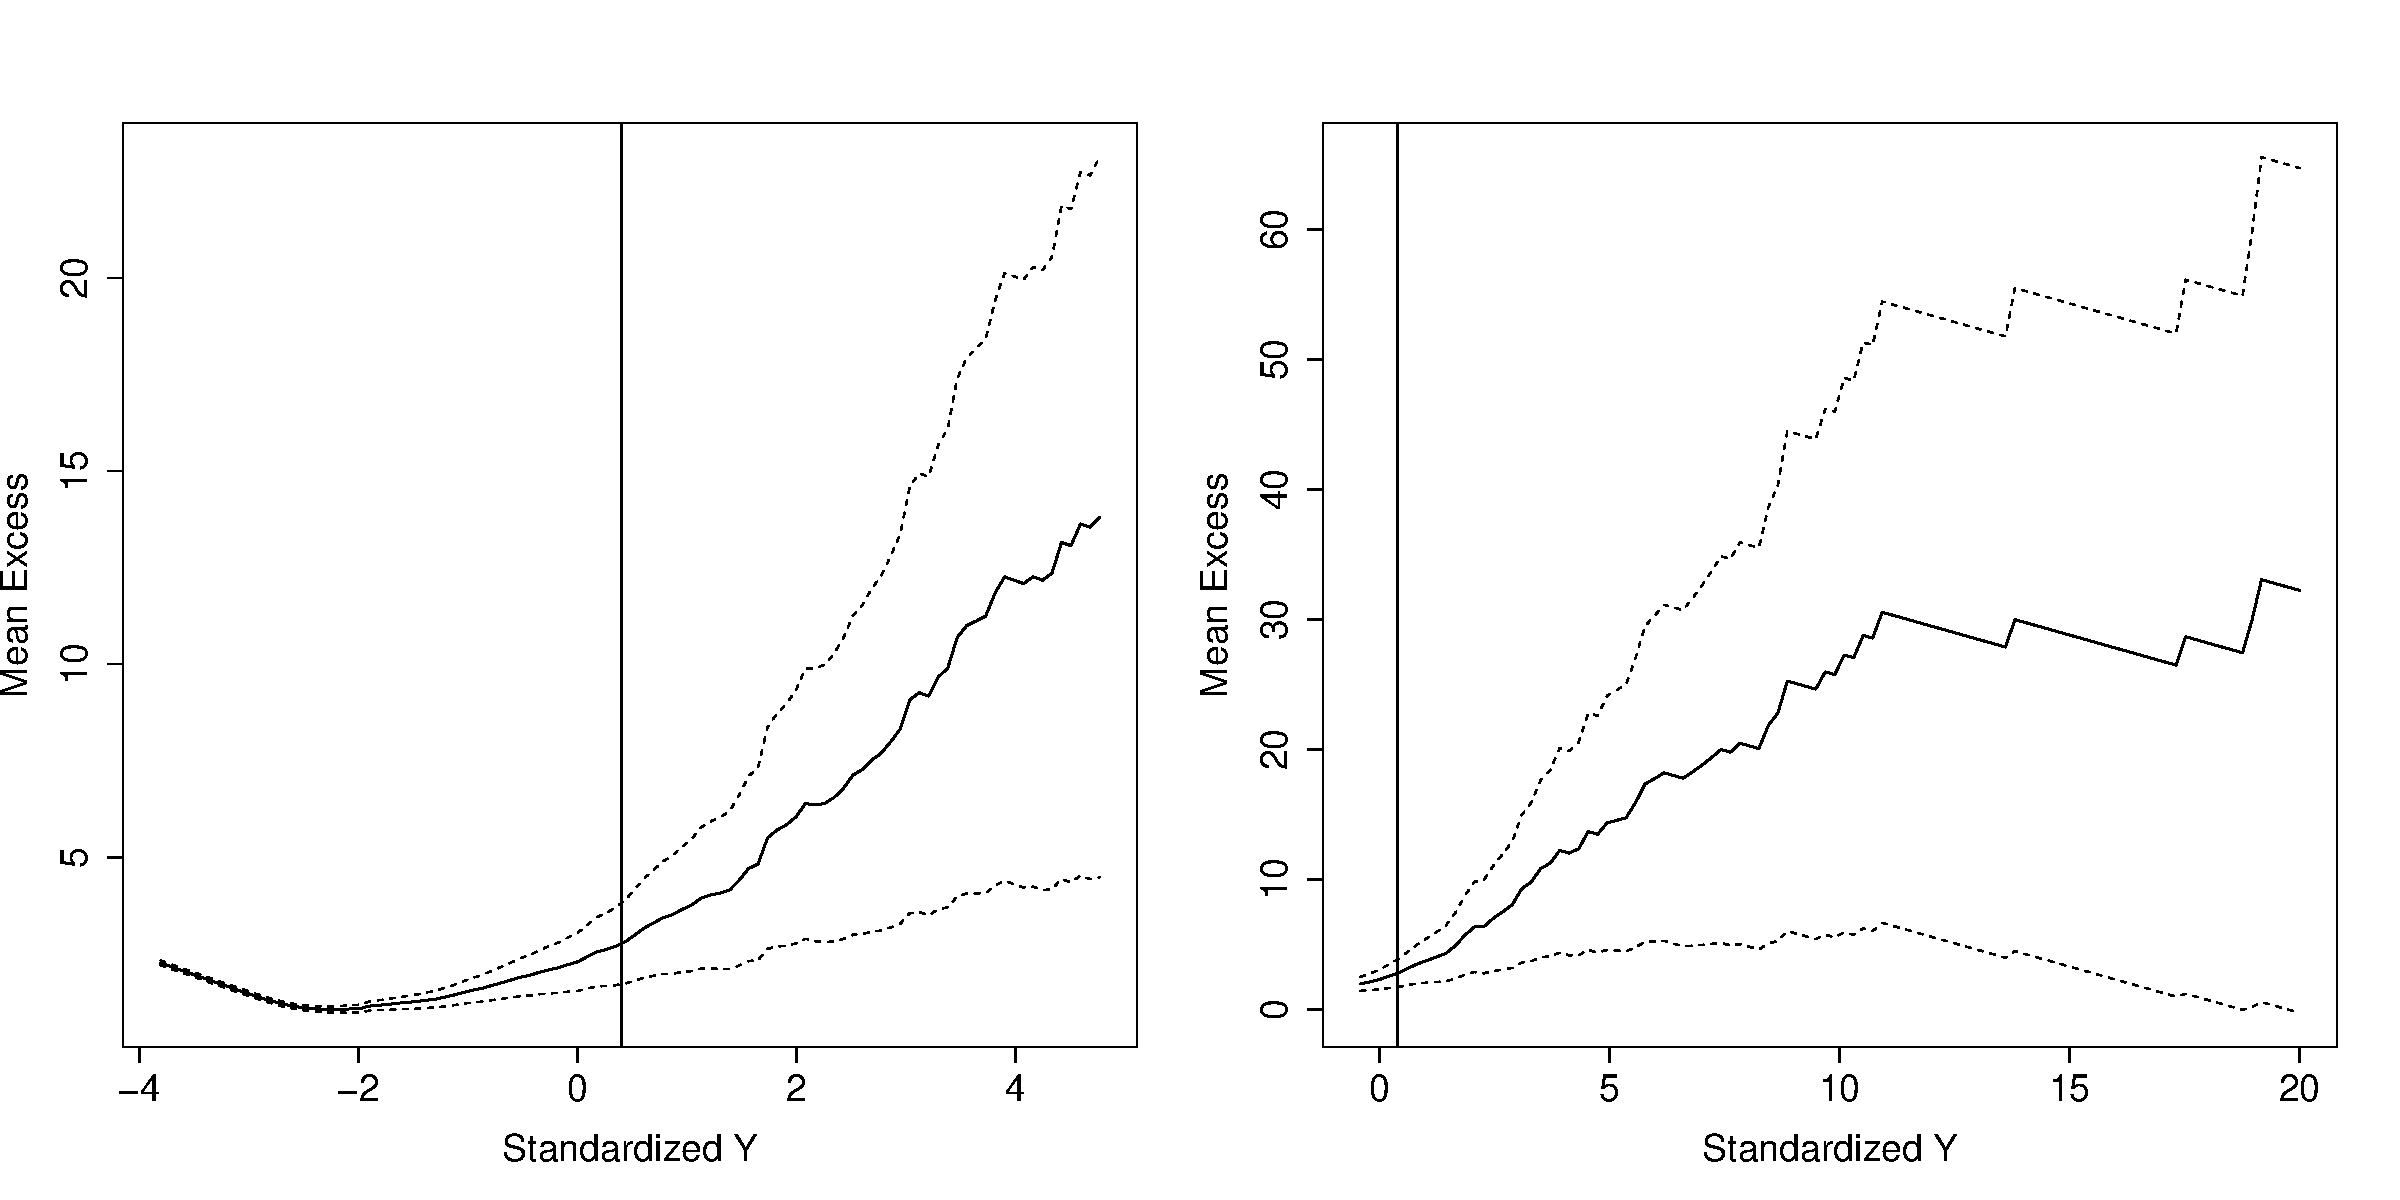
\includegraphics[width=1\textwidth]{fire-mrl-plots}

		Mean residual life plot for fire data. Vertical line at sample 95th quantile.
	\end{center}
\end{frame}

\begin{frame}{Fire: 95th percentile by county, $T(\bs)$}\vspace{-35pt}
	\begin{center}
		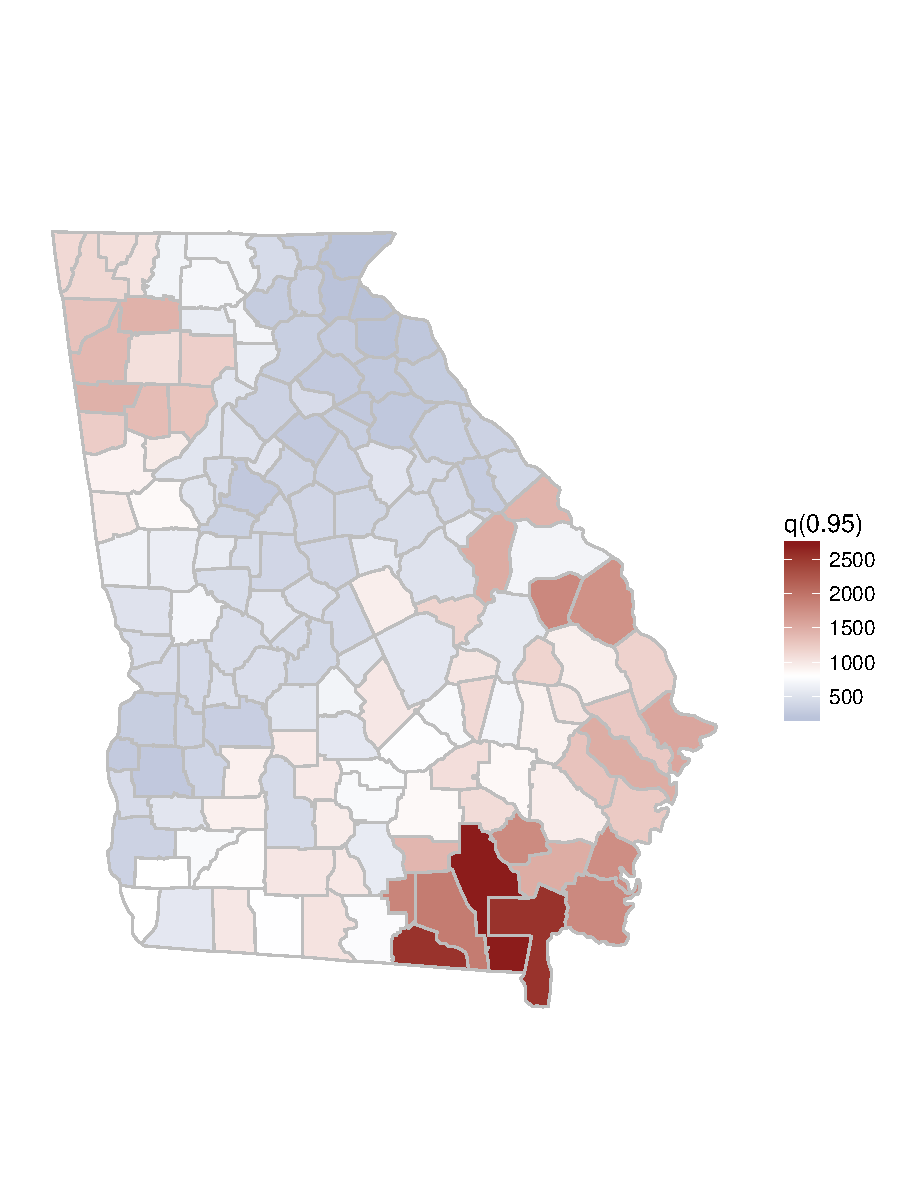
\includegraphics[height=0.95\textheight]{fire-spatial-q95}
		\vspace{-3em}

		Spatially smoothed 95th percentile.
	\end{center}
\end{frame}

%\begin{frame}{Model comparisons - TODO}
%	\begin{center}
%		\begin{tabular}{rcc}
%			\toprule
%			$L$ & Brier Score & Quantile score\\
%			\midrule
%			5   & 5.64 & 135.7 \\
%			10  & 5.33 & 127.3 \\
%			15  & 5.00 & 128.3 \\
%			20  & 4.93 & 122.4 \\
%			{\bf 25}  & {\bf 4.78} & {\bf 116.9} \\
%			40  & 4.72 & 115.7\\
%			\bottomrule
%		\end{tabular}
%	\end{center}
%\end{frame}

\begin{frame}{Fire: EBF weights, $v_l$}
	\begin{center}
		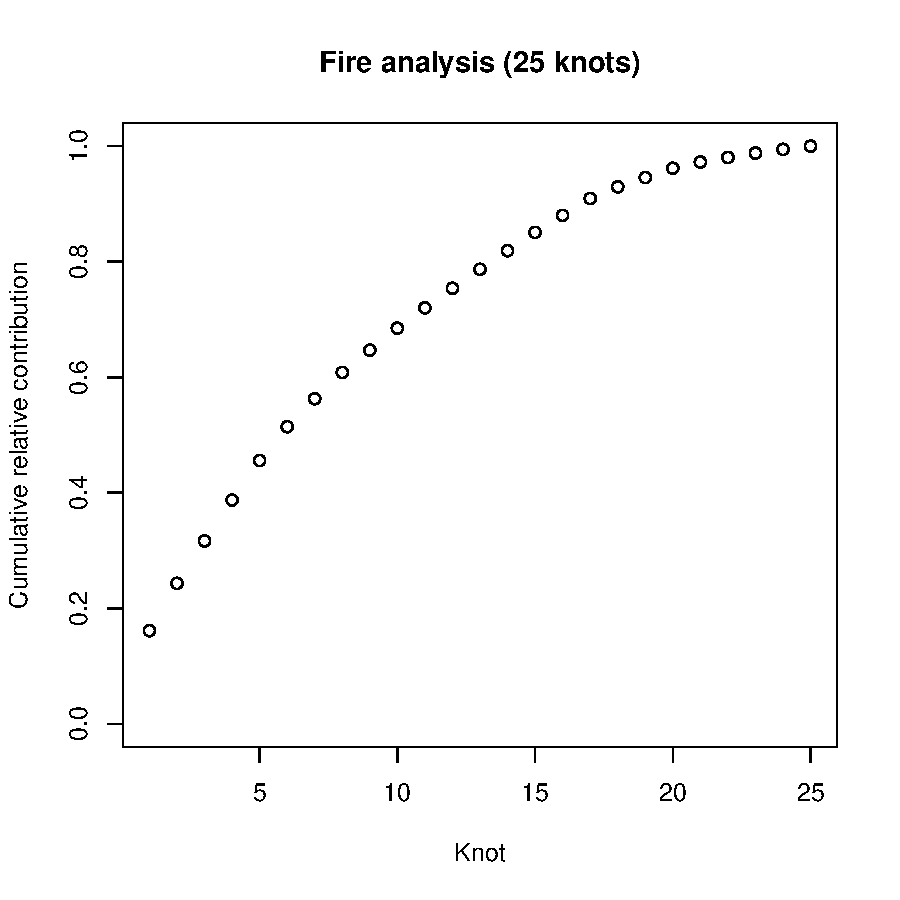
\includegraphics[height=0.9\textheight]{firev-25}
	\end{center}
\end{frame}

\begin{frame}{Fire: EBF's $B_l(\bs)$}
	\begin{center}
		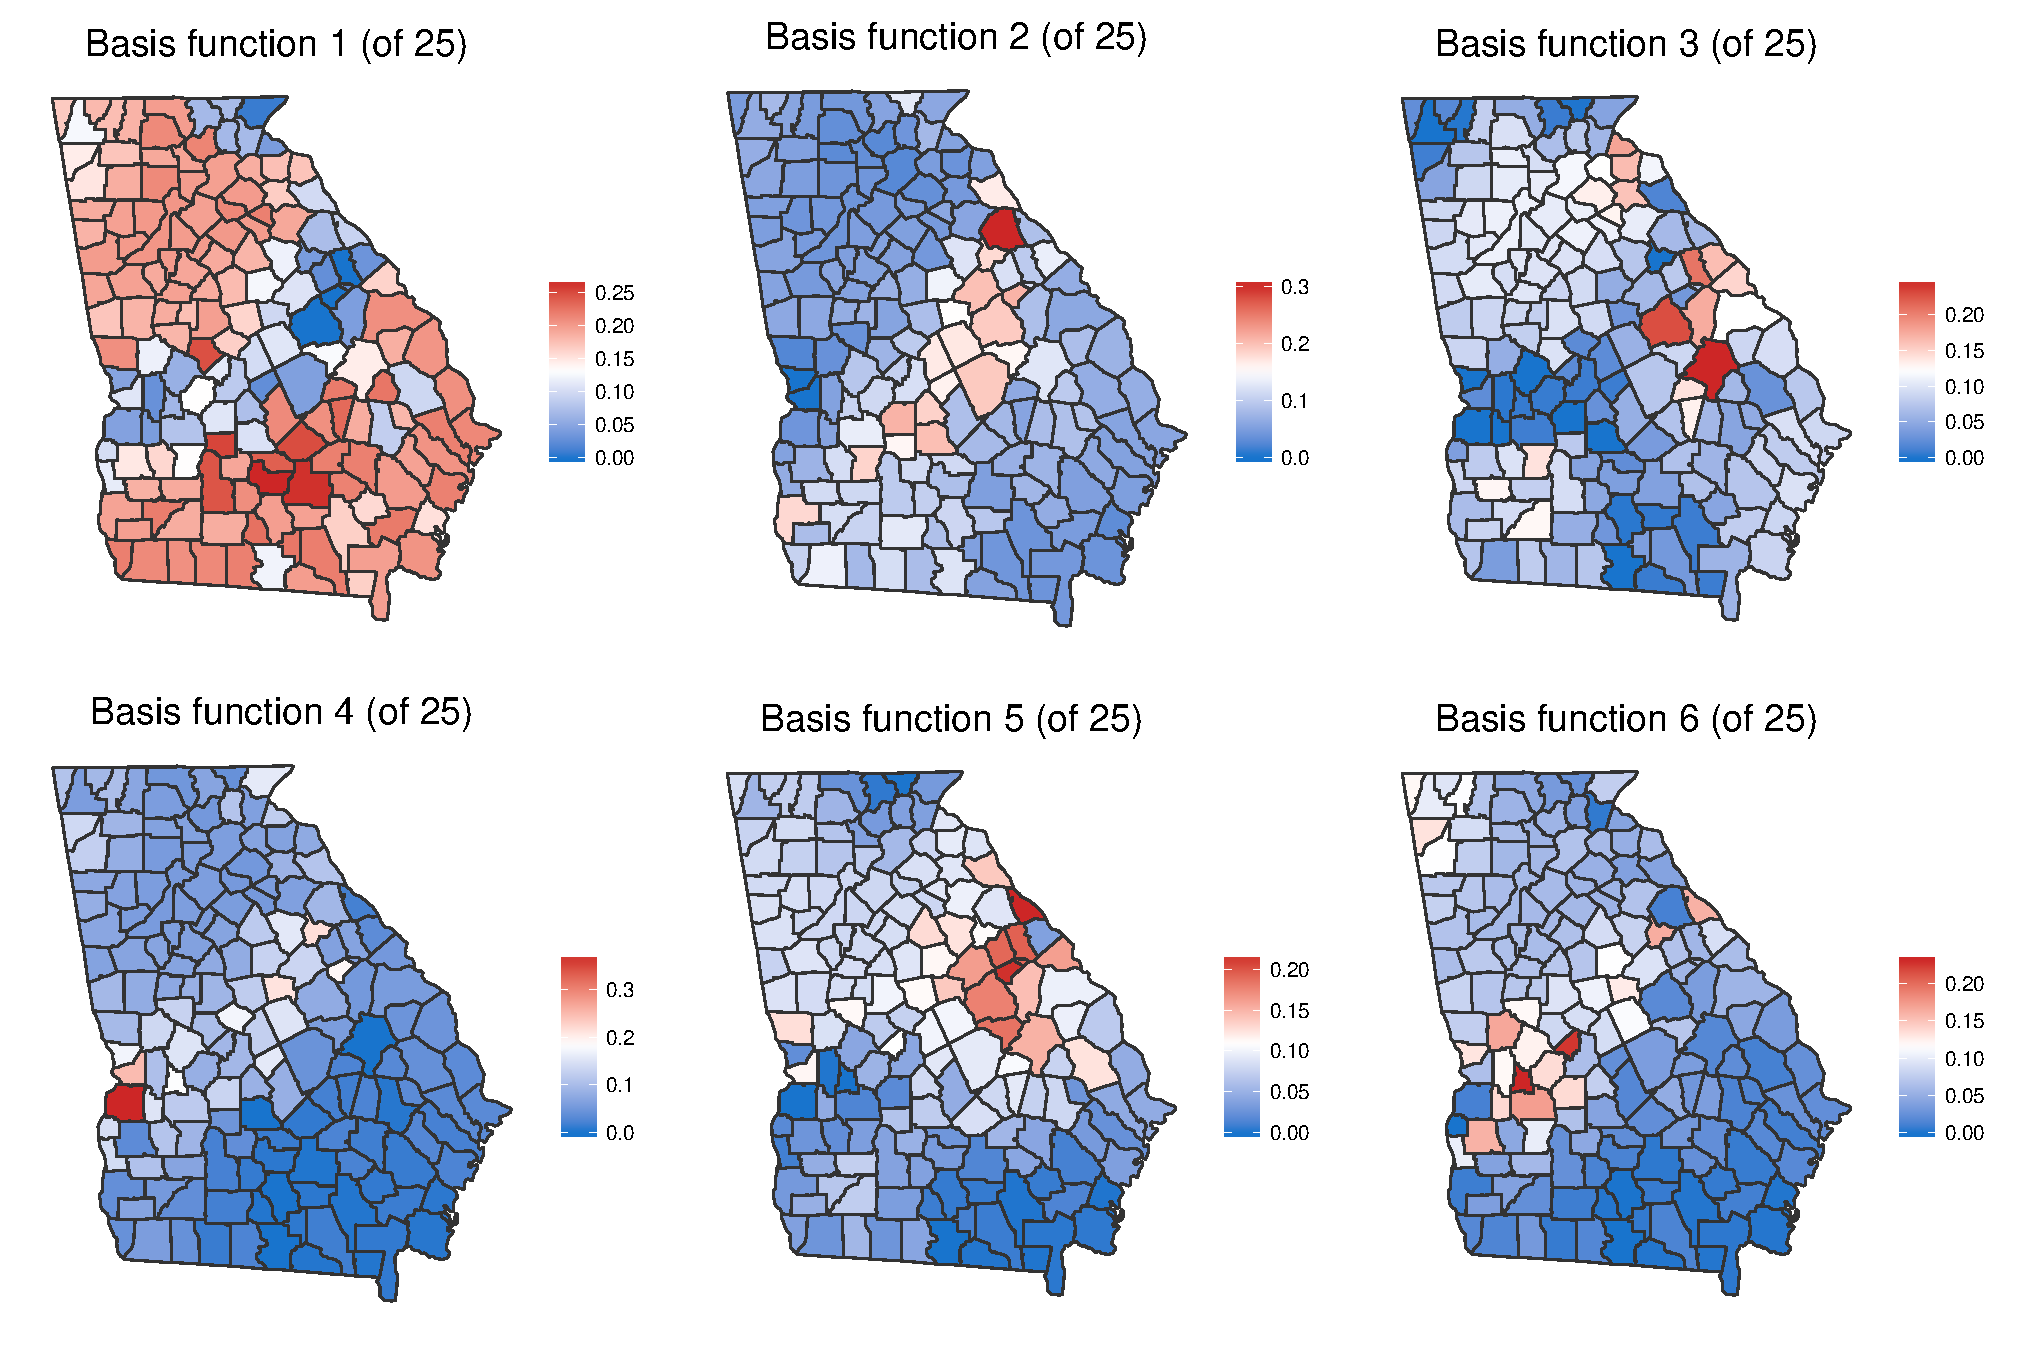
\includegraphics[width=0.9\textwidth]{fire-ebf-panel}
	\end{center}
\end{frame}

%\begin{frame}{GA Fires -- Ecoregions}
%	\begin{center}
%		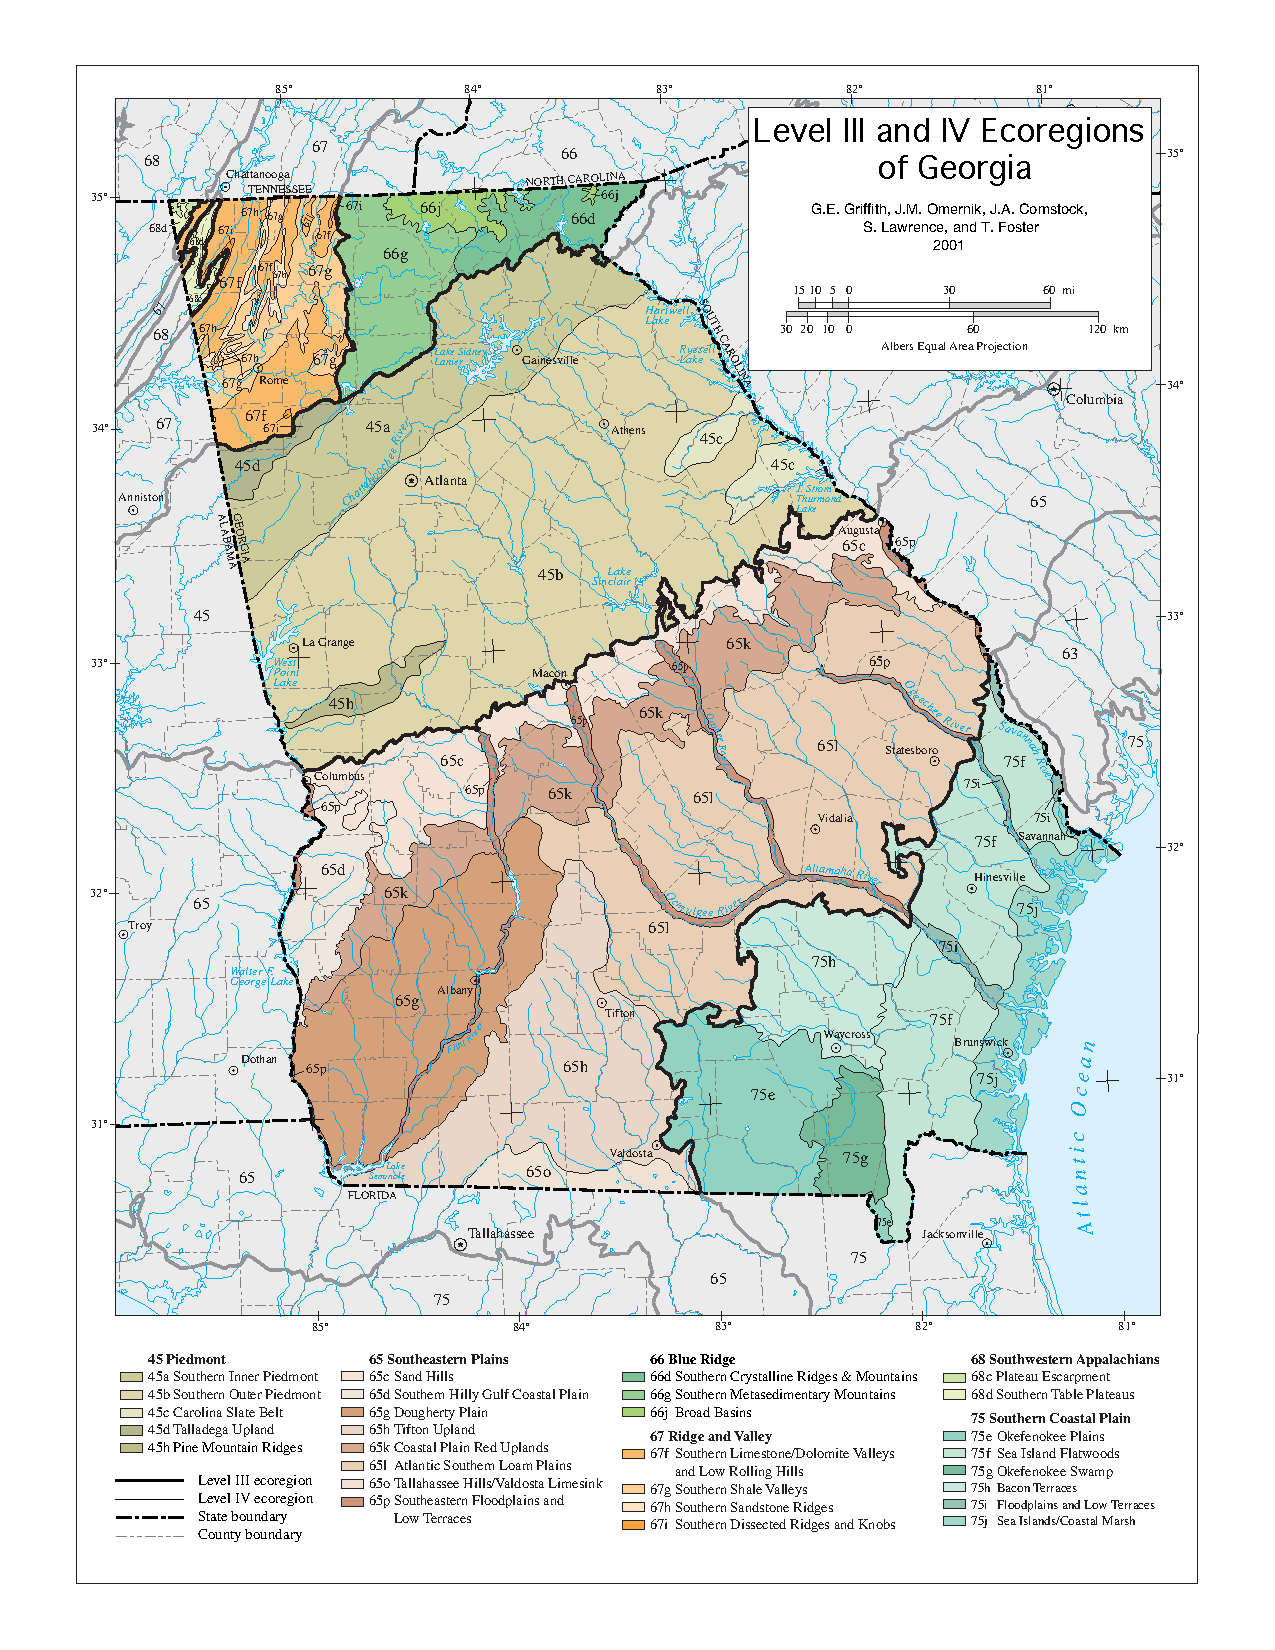
\includegraphics[height=0.9\textheight]{ga_eco_regions}
%	\end{center}
%\end{frame}

\begin{frame}{Fire: Posterior summaries ($L = 25$)}
	\begin{center}
		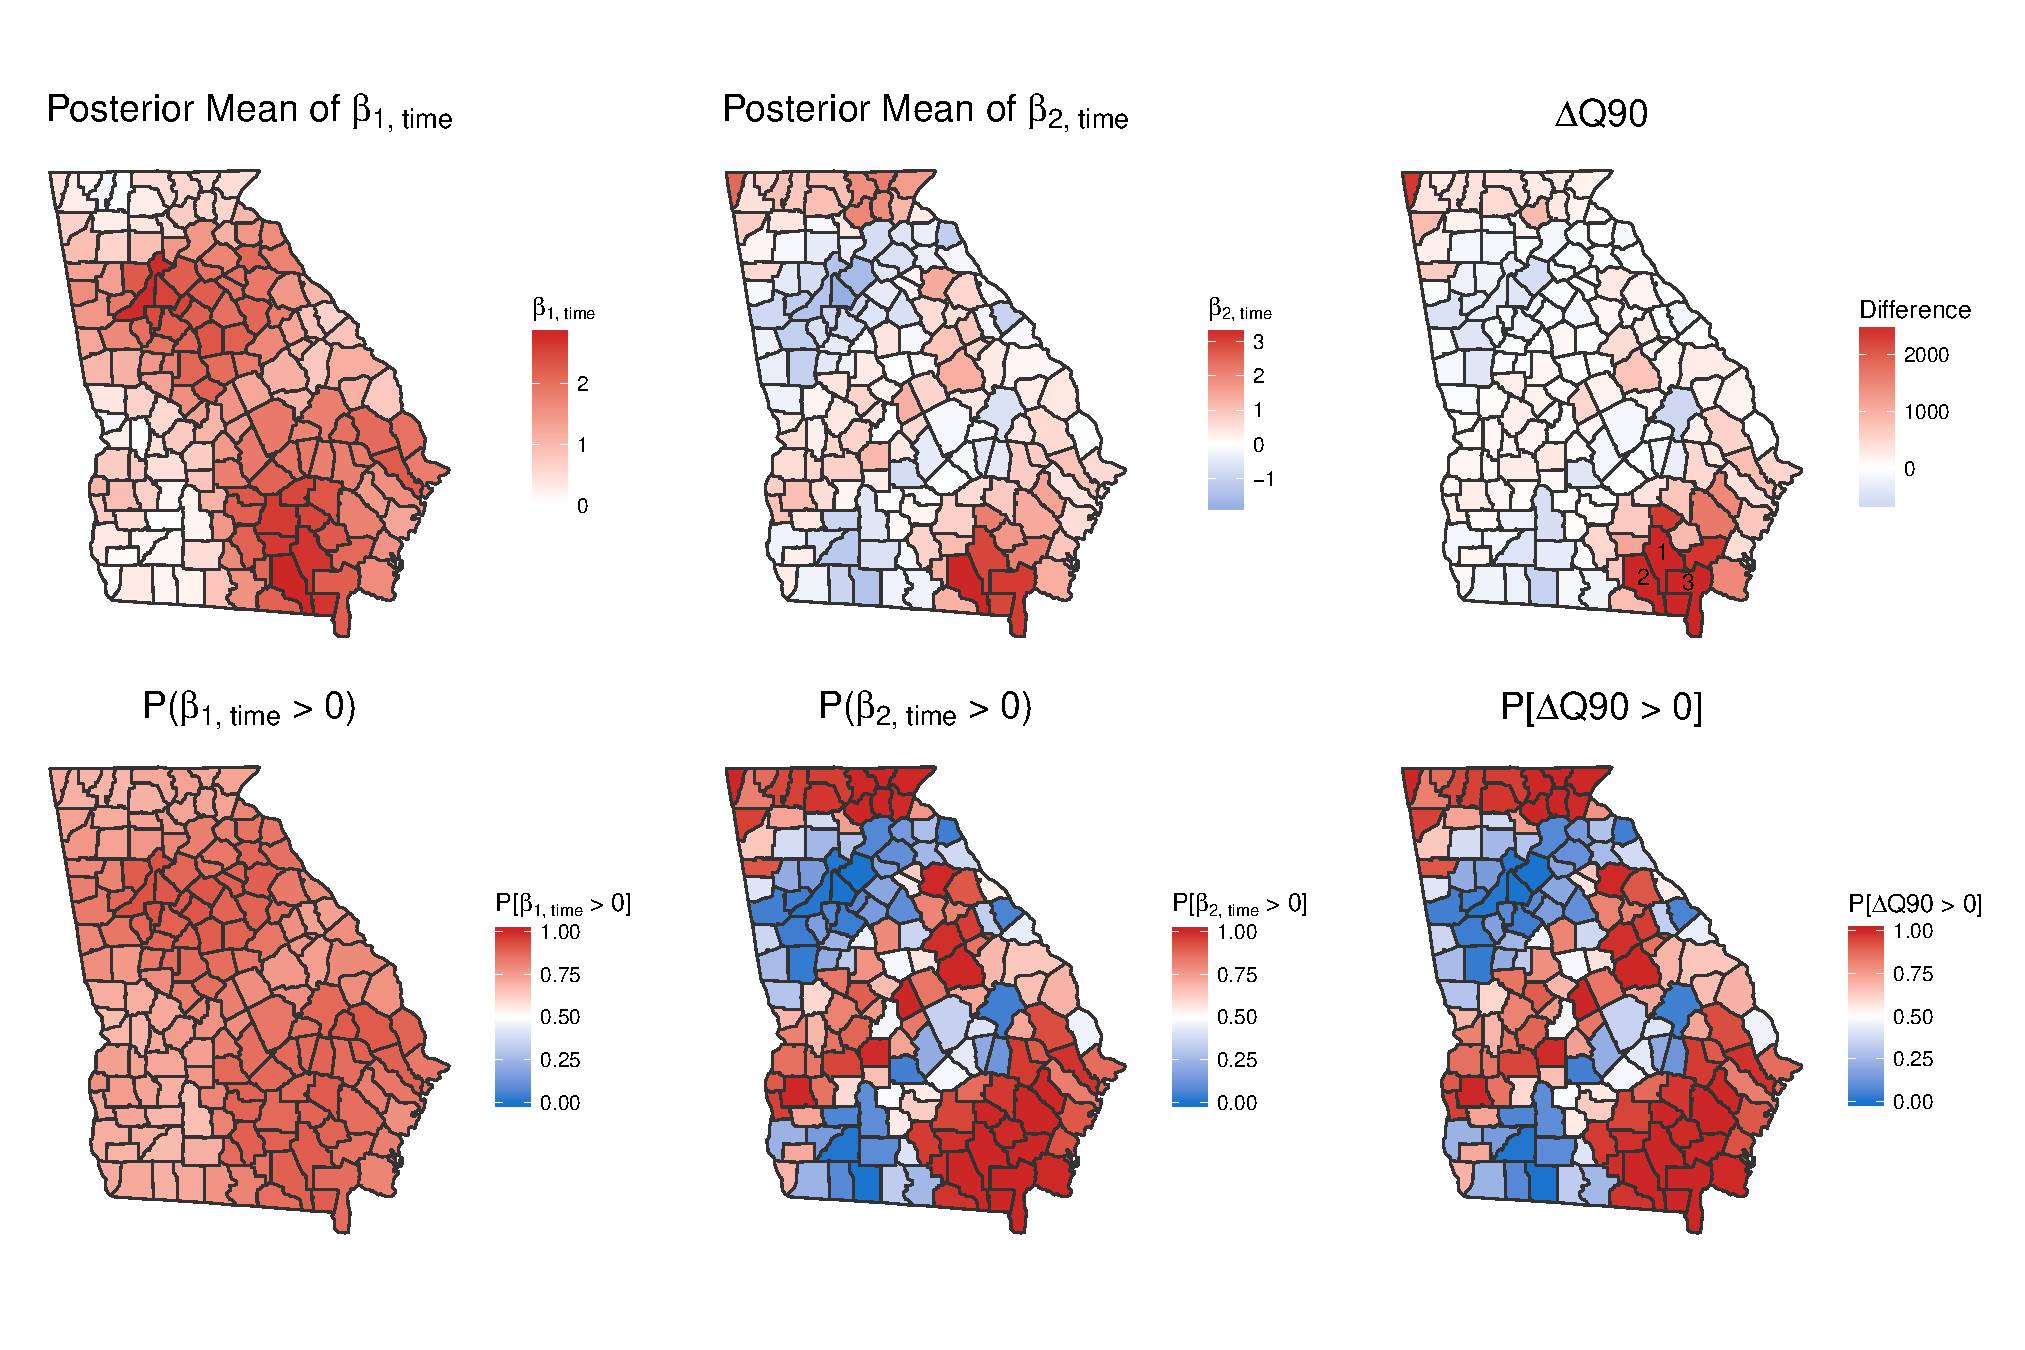
\includegraphics[width=0.9\textwidth]{fire-ebf-postpanel-slides}
	\end{center}
\end{frame}

%\begin{frame}{Fire: Time trend for $\log[\sigma(\bs)]$}
%	\begin{center}
%		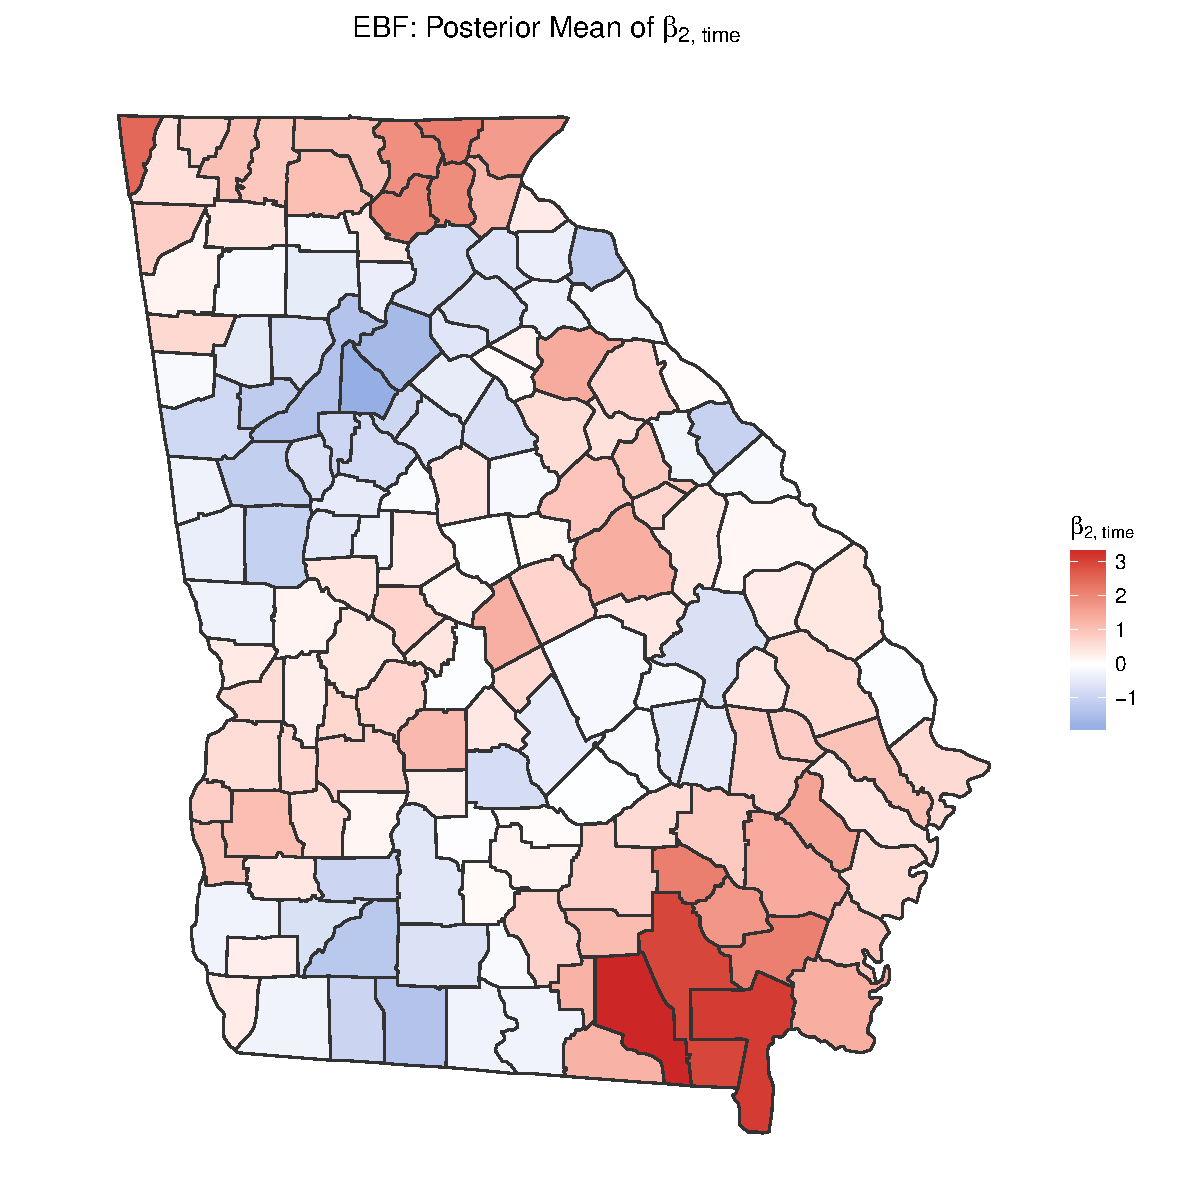
\includegraphics[width=\textwidth]{fire-ebf-post-beta2time}
%	\end{center}
%\end{frame}
%
%\begin{frame}{Fire: Time trend for $Q(90)$}
%	\begin{center}
%		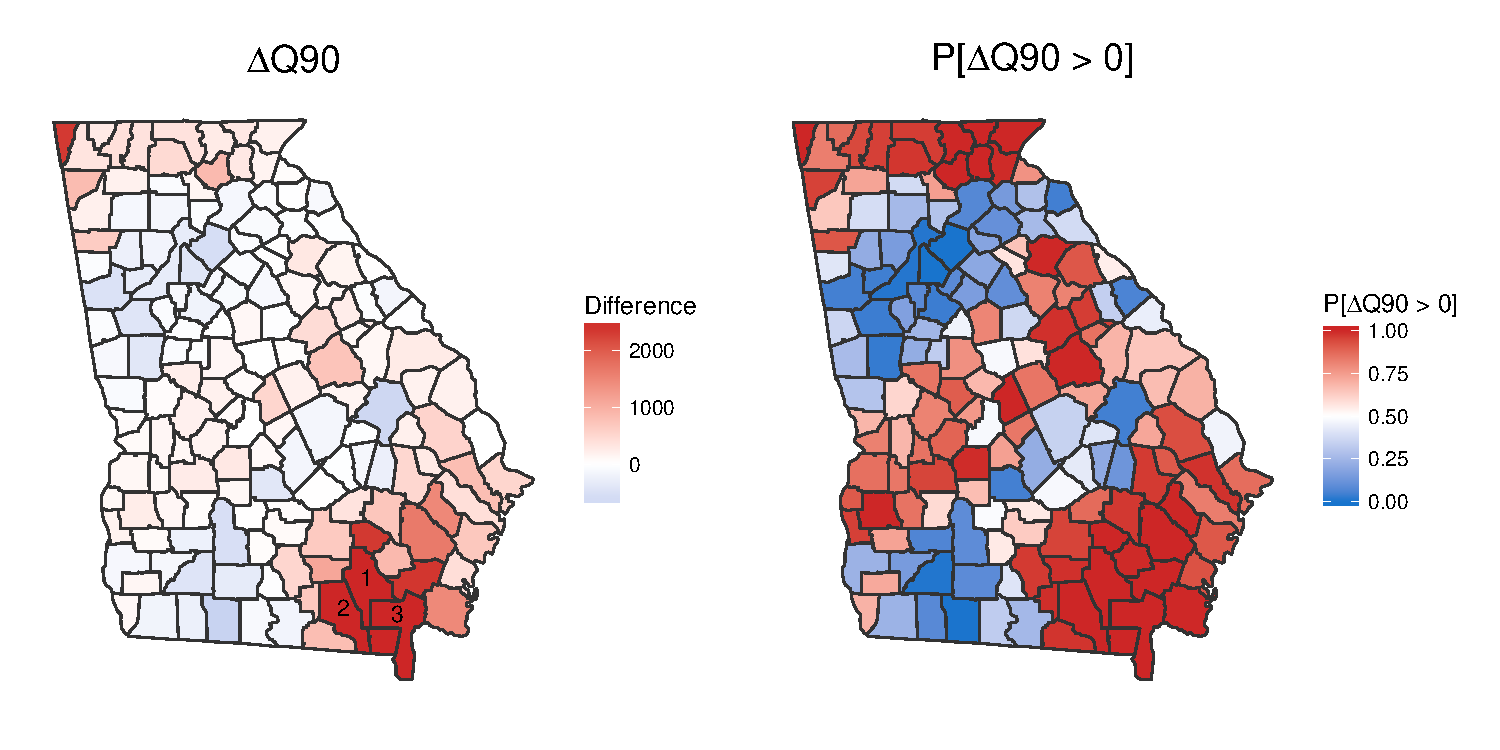
\includegraphics[width=\textwidth]{fire-ebf-post-q90diff}
%	\end{center}
%\end{frame}

\begin{frame}{Application 2: NARCCAP climate model output}
	\begin{itemize}\setlength{\itemsep}{1em}
		\item Data consist of annual maximum precipitation at 697 grid cells in the Eastern US
		\item Model is run separately for 1969--2000 and 2039--2077
		\item The objective is to compare the extremes in the two climate periods
		\item We fit the same model as for the fire data except without censoring
	\end{itemize}
\end{frame}


\begin{frame}{Climate model output for 1969}
	\begin{center}
		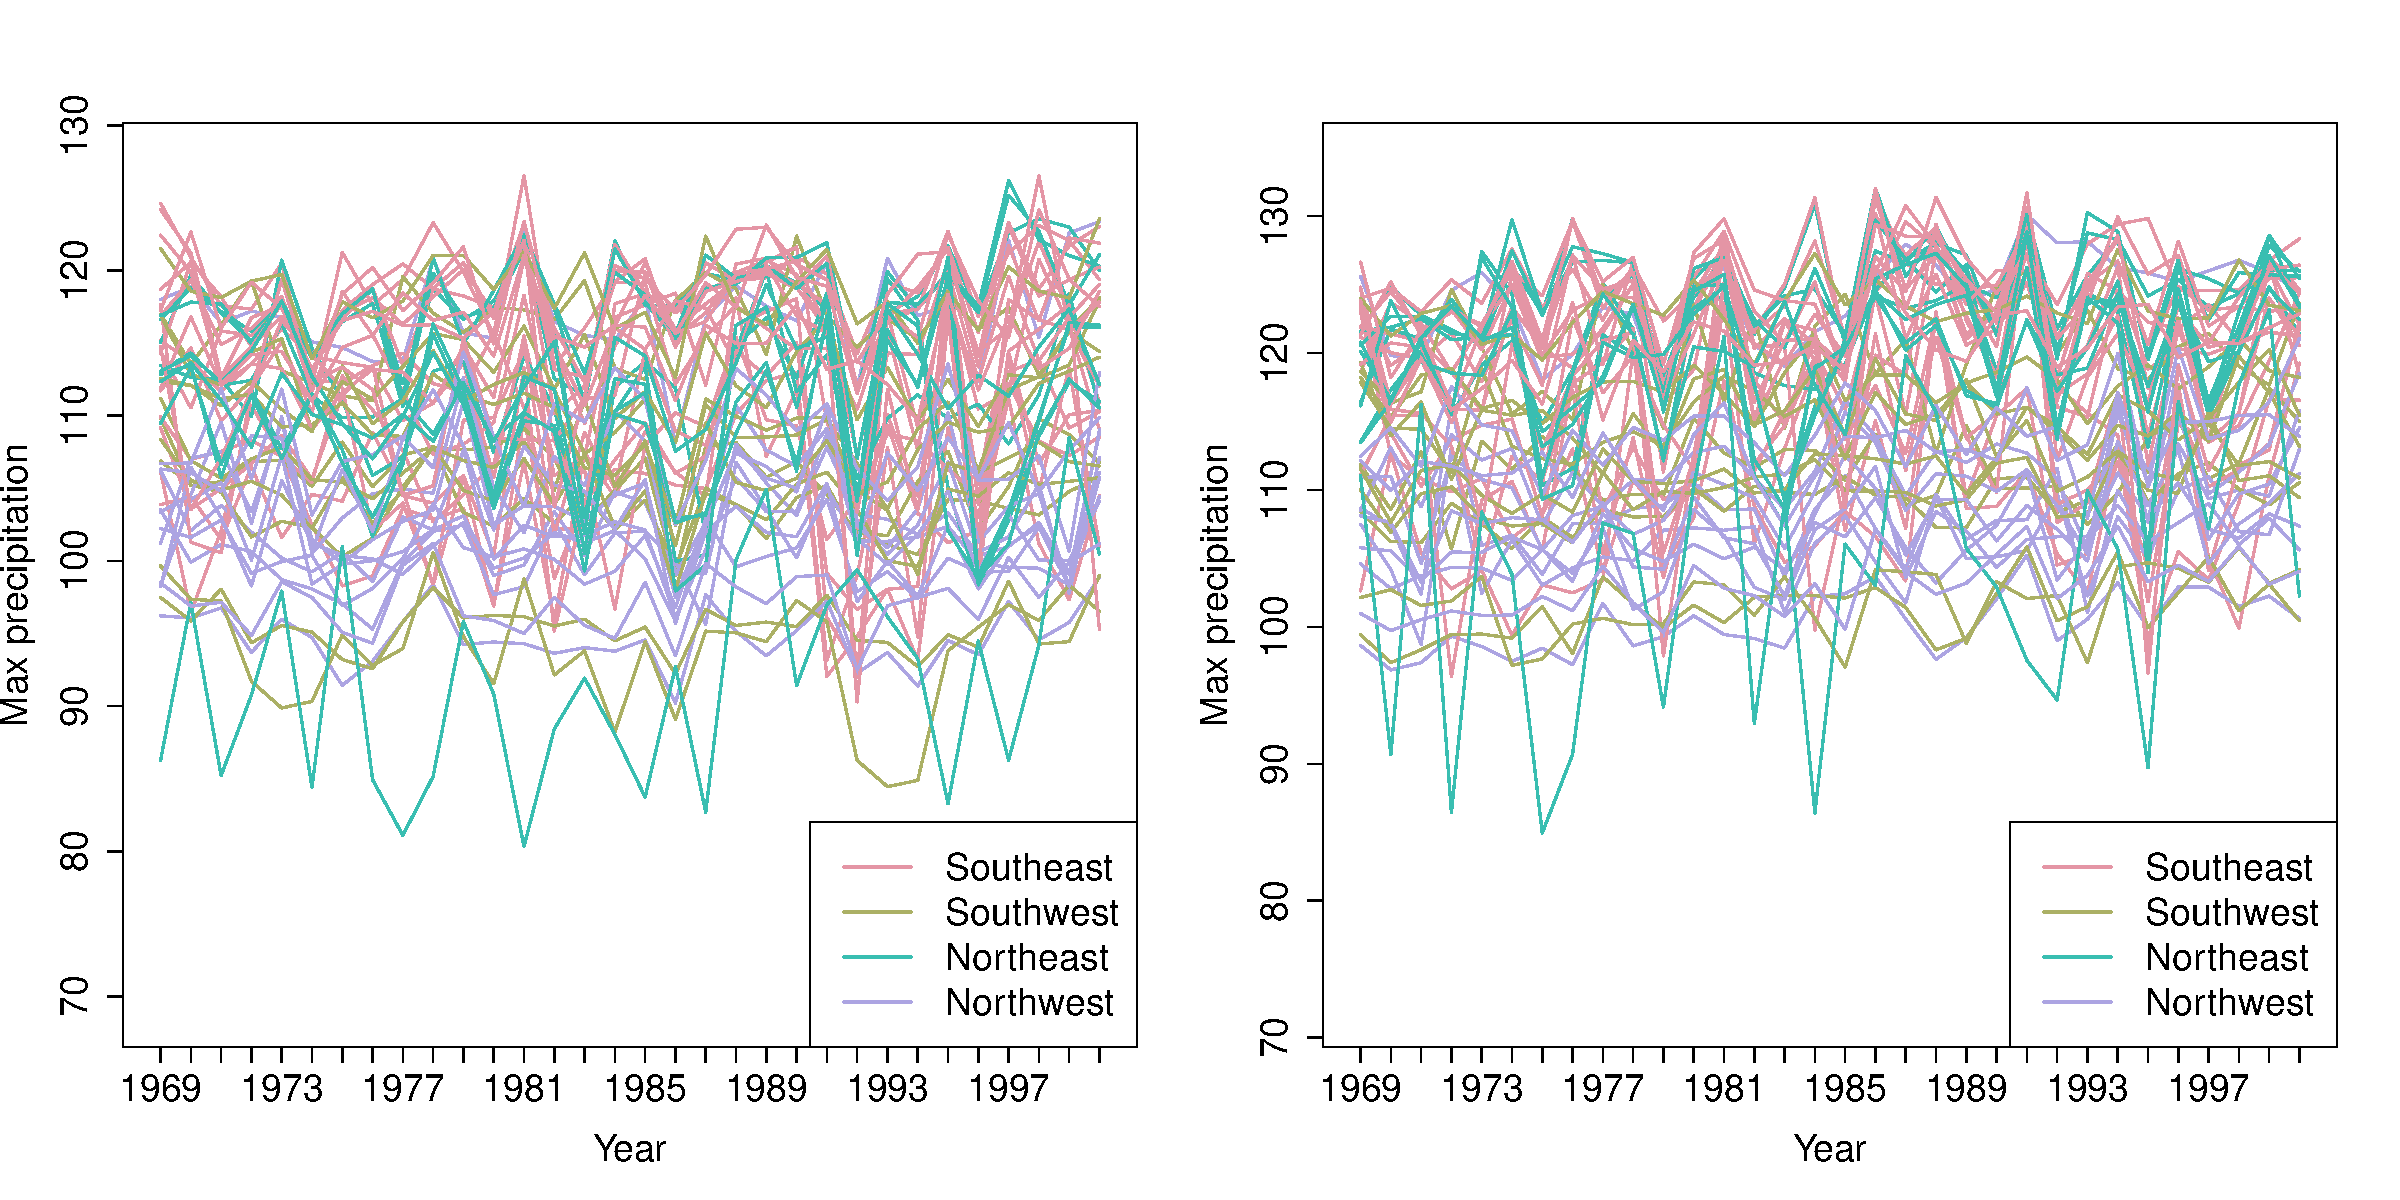
\includegraphics[width=\textwidth]{precip-ts}
	\end{center}
\end{frame}

\begin{frame}{Precip: EBF weights, $v_l$}
	\begin{center}
		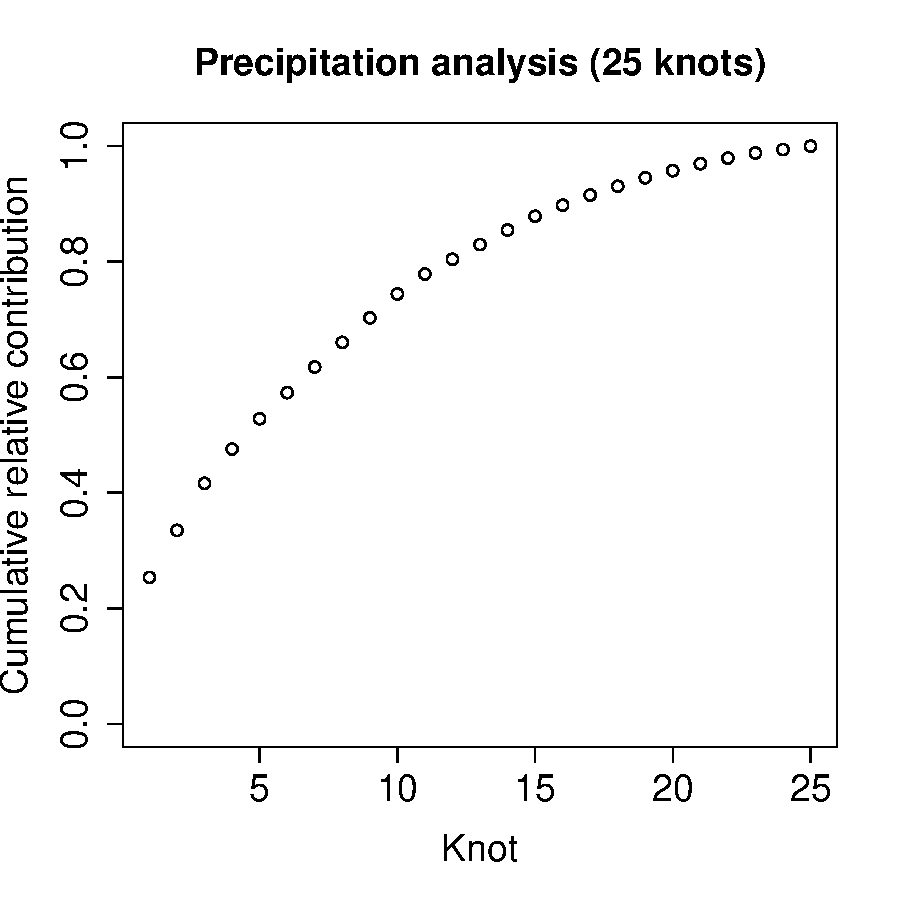
\includegraphics[height=0.85\textheight]{precipv-25}
	\end{center}
\end{frame}

\begin{frame}{Precip: EBFs $B_l(\bs)$}
	\begin{center}
		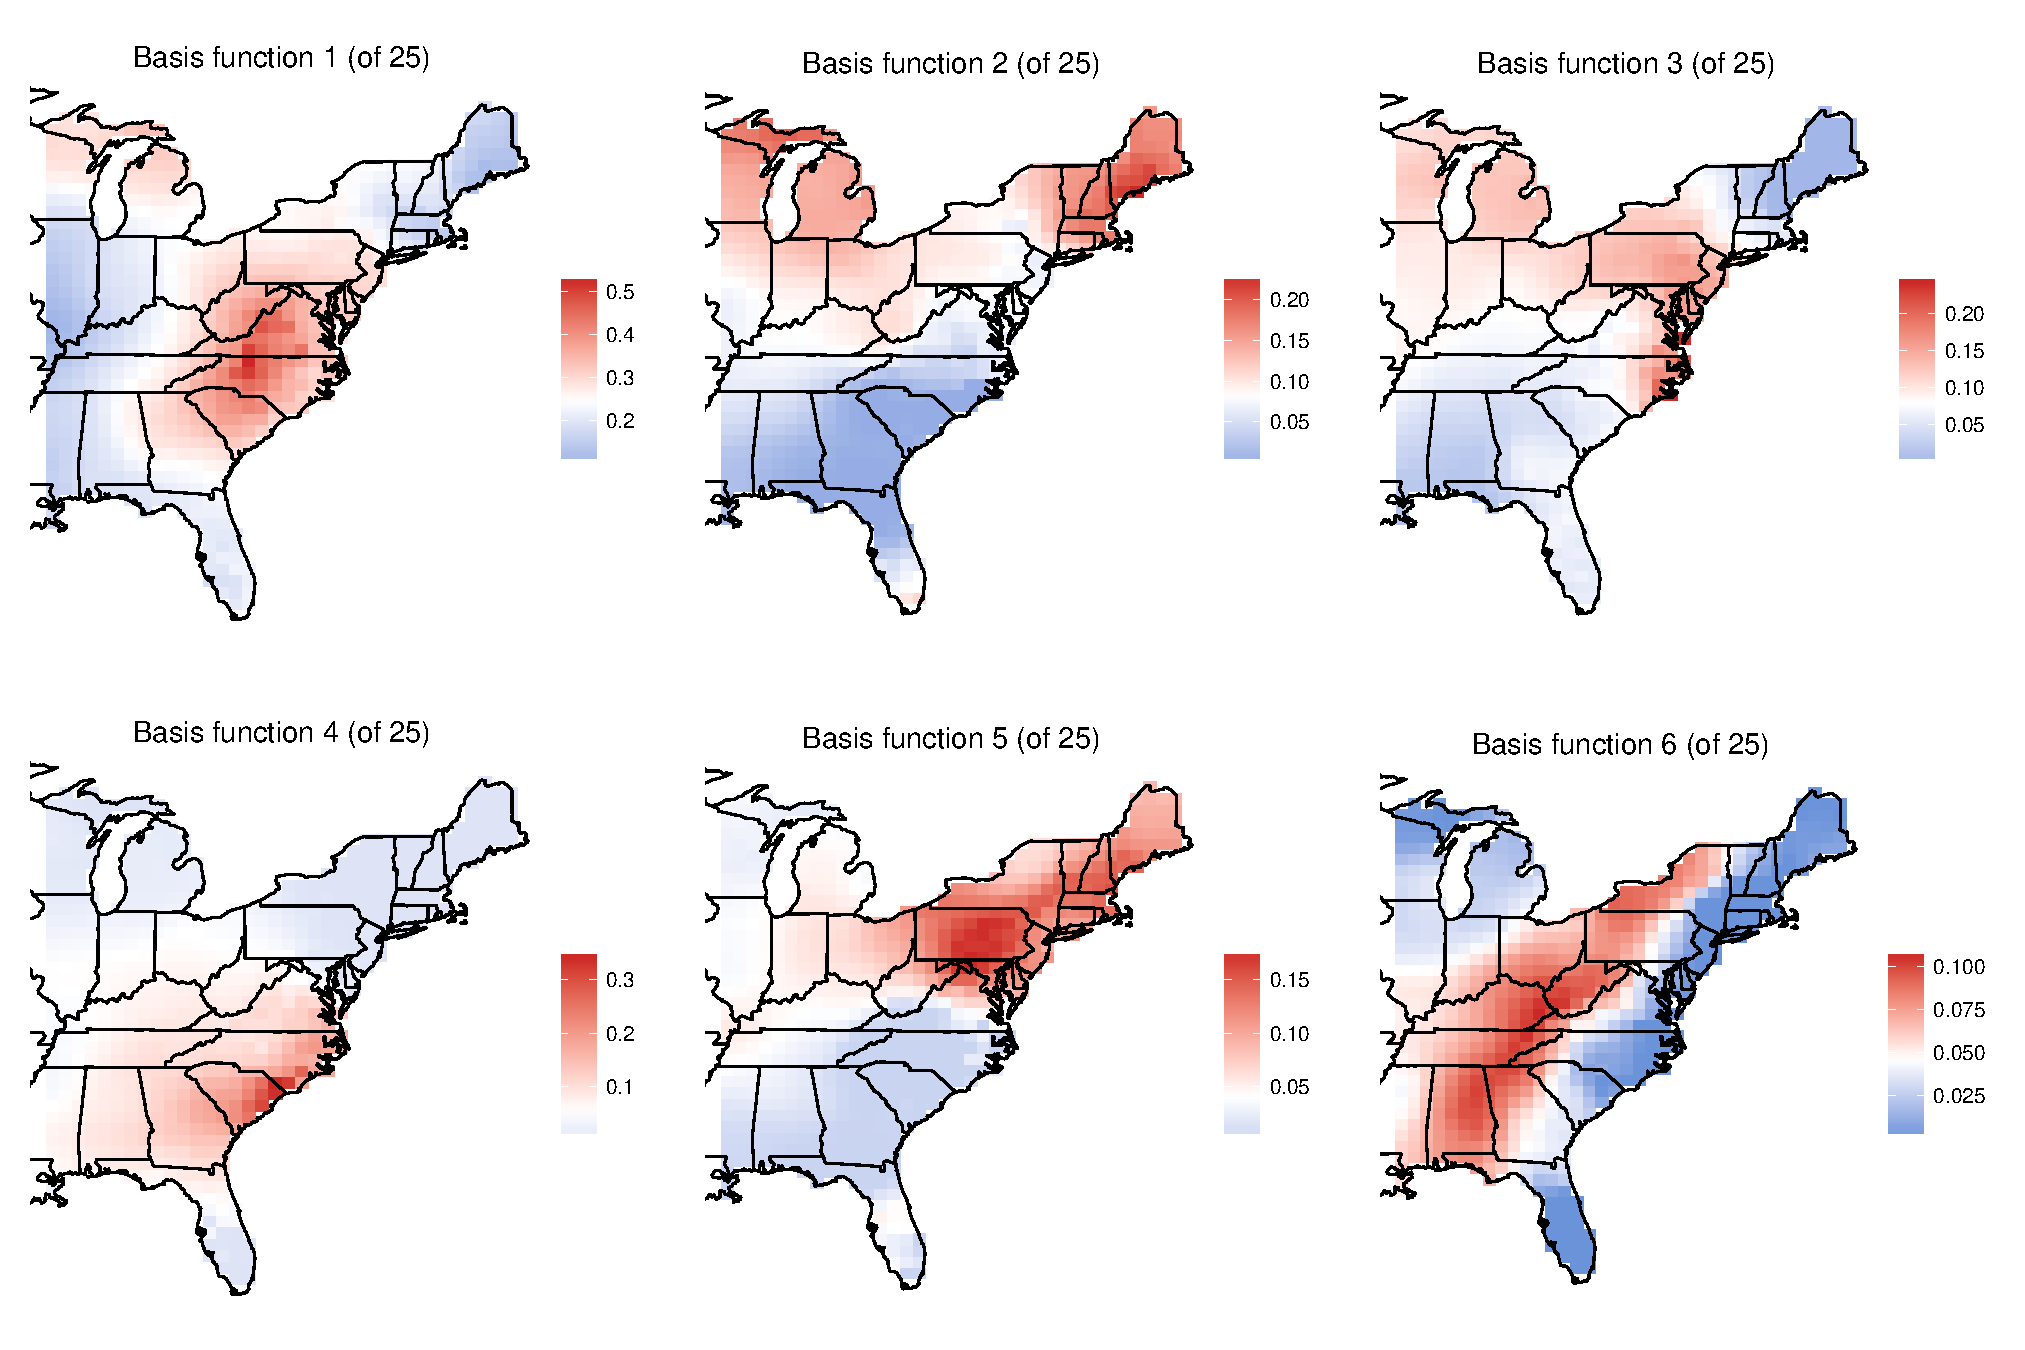
\includegraphics[width=0.9\textwidth]{precip-ebf-panel}
	\end{center}
\end{frame}

\begin{frame}{Precip: Posterior summaries ($L = 25$)}
	\begin{center}
		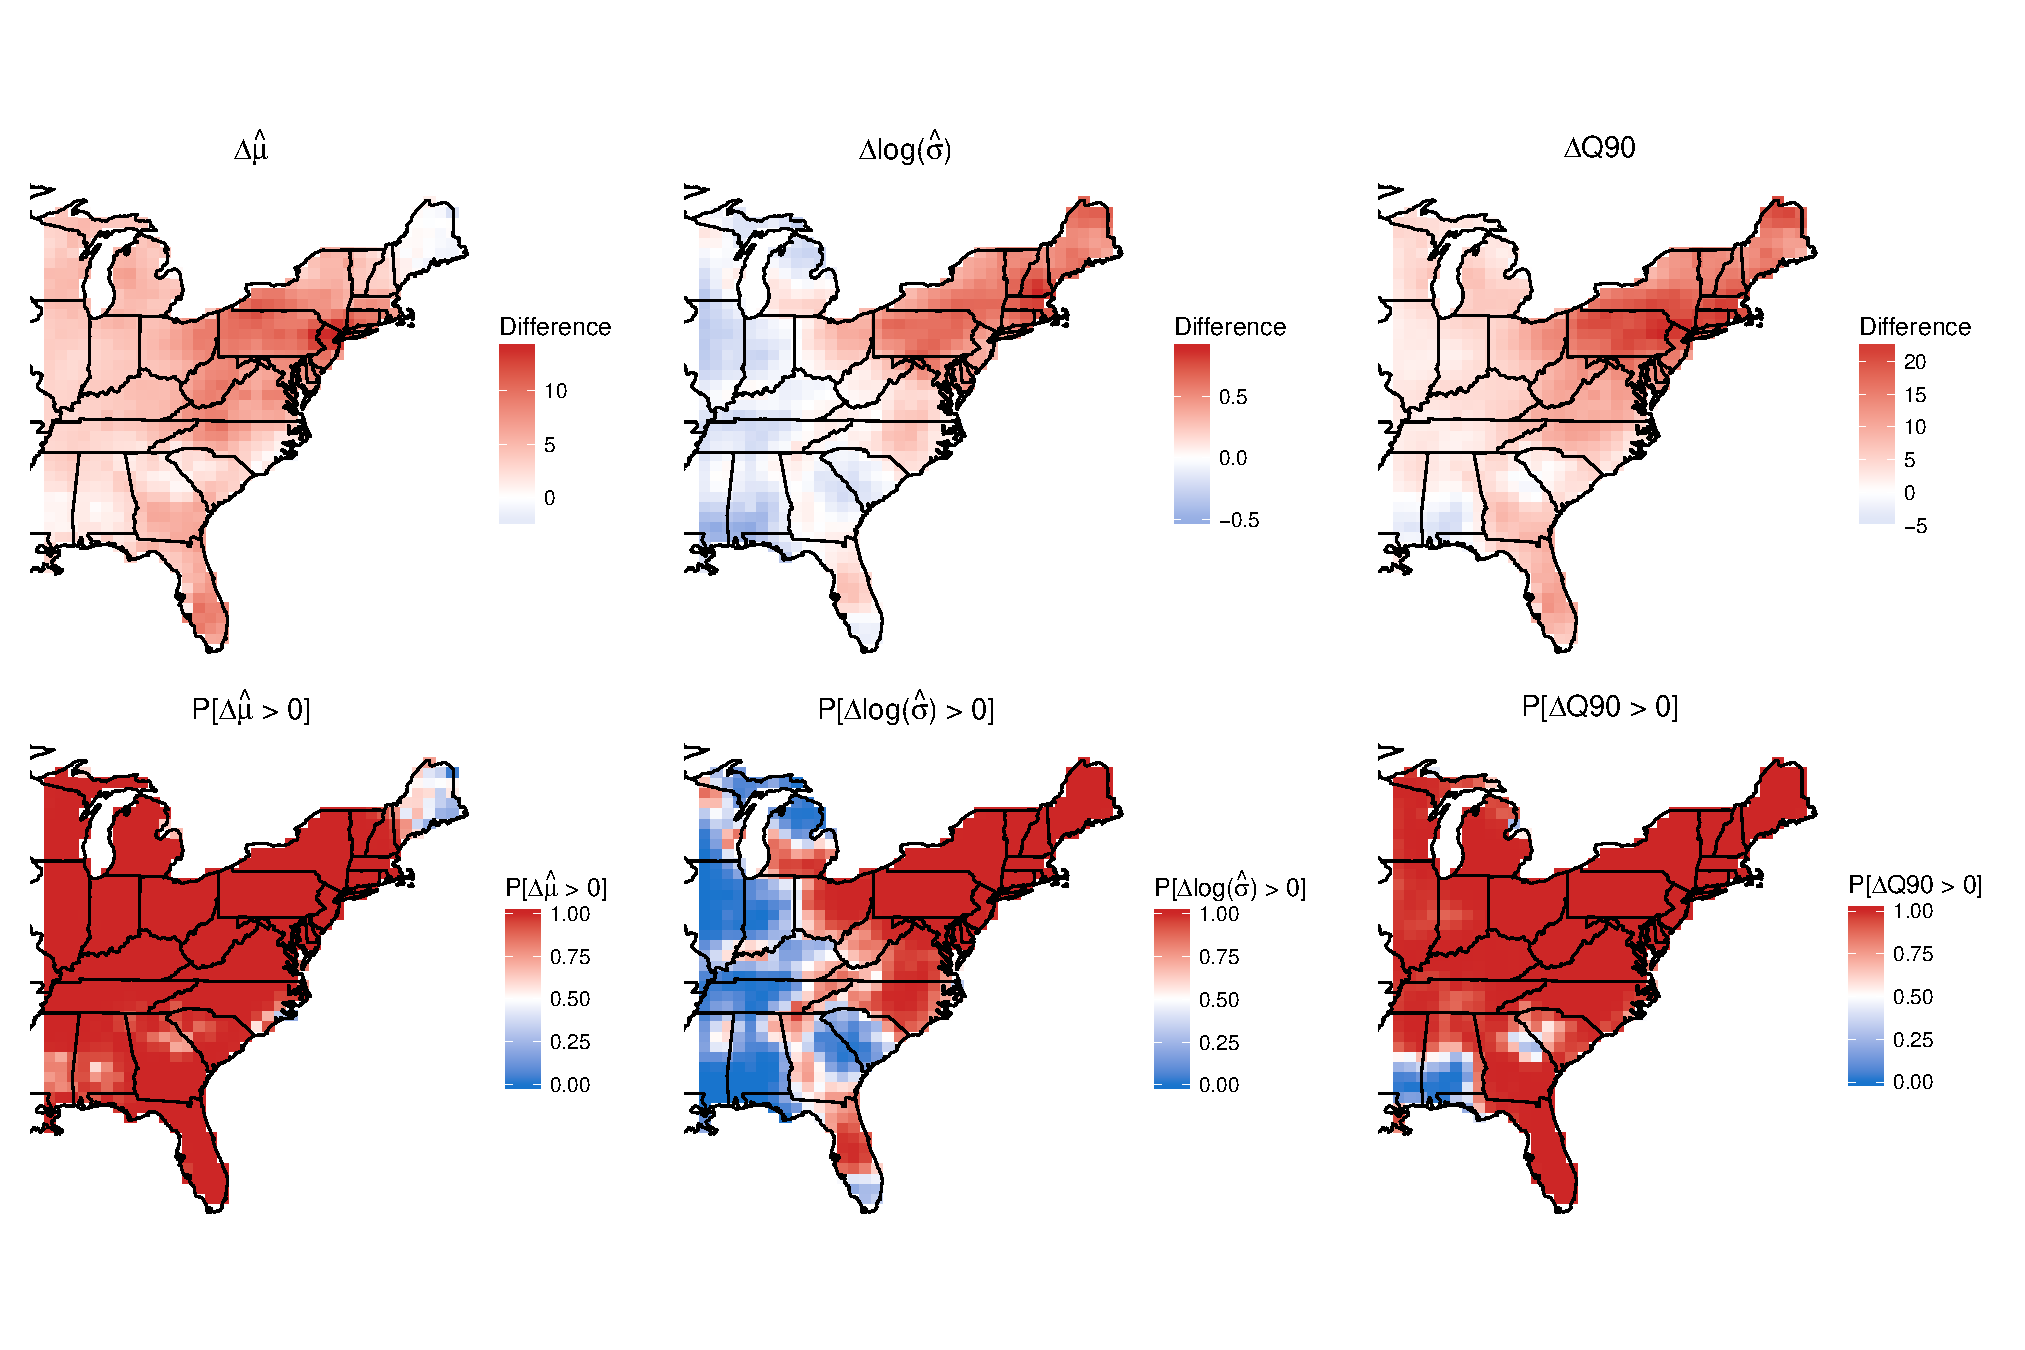
\includegraphics[width=0.9\textwidth]{precip-ebf-postpanel-slides}
	\end{center}
\end{frame}

\begin{frame}{Results}
	\begin{itemize} \setlength{\itemsep}{1em}
    \item Comparison to principal components: \vspace{0.5em}
    \begin{itemize} \setlength{\itemsep}{0.5em}
		  \item For fire data, EBFs and PCAs are different due to censoring
		  \item For precipitation data, EBFs and PCAs generally capture similar features
    \end{itemize}
		\item EBF performs better than standardized Gaussian kernel functions when there is spatial dependence in the data \vspace{0.5em}
    \begin{itemize} \setlength{\itemsep}{0.5em}
      \item Fire: $\hat{\alpha} = 0.86$
      \item Precipitation: $\hat{\alpha} = 0.28$
    \end{itemize}
	\end{itemize}
\end{frame}

%\begin{frame}{Precip: Time trend for $\log[\sigma(\bs)]$}
%	\begin{center}
%		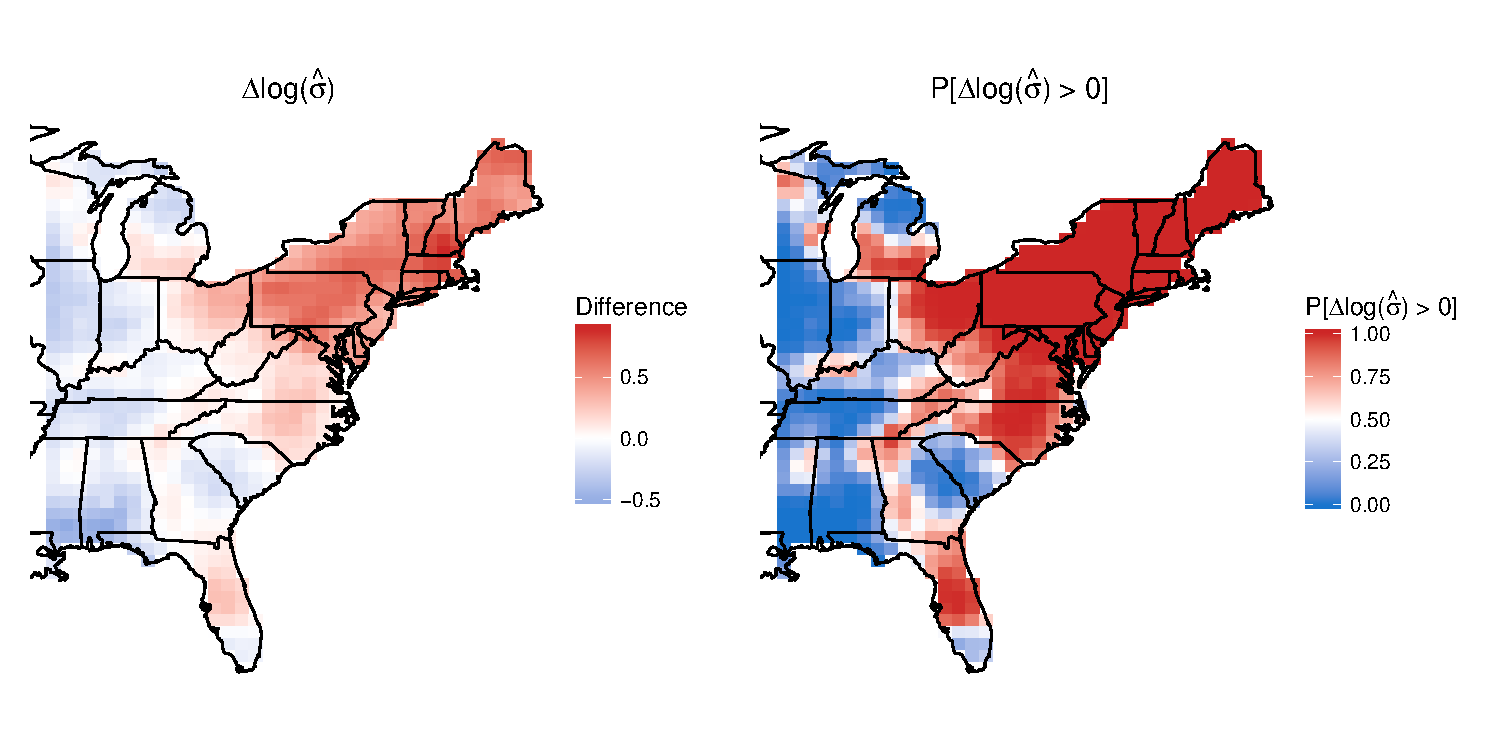
\includegraphics[width=\textwidth]{precip-ebf-post-beta2time}
%	\end{center}
%\end{frame}
%
%\begin{frame}{Precip: Time trend for $Q(90)$}
%	\begin{center}
%		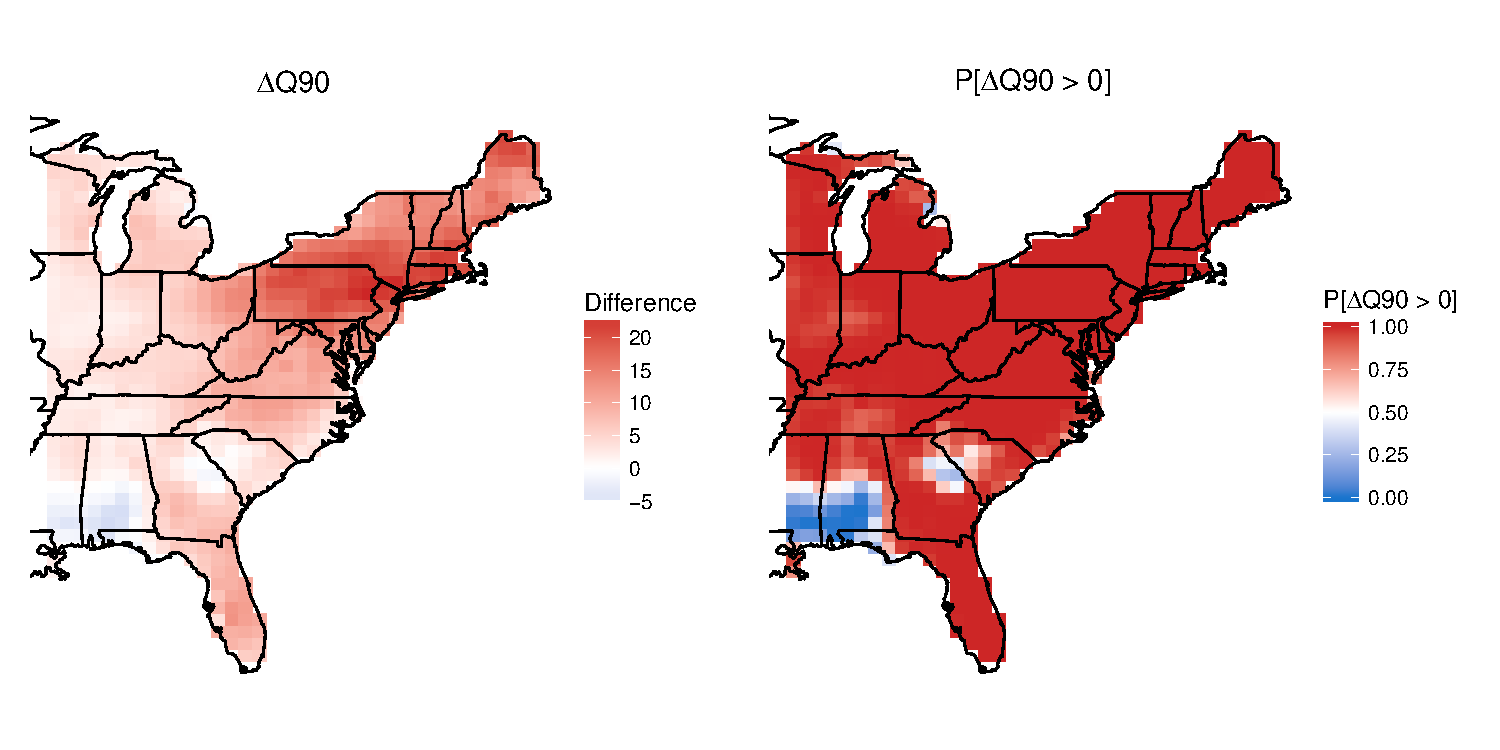
\includegraphics[width=\textwidth]{precip-ebf-post-q90diff}
%	\end{center}
%\end{frame}


\begin{frame}{Questions}
	\begin{itemize} \setlength{\itemsep}{1em}
		\item Thank you for your attention.
    \item Questions?
		\item Acknowledgment: This work was funded by EPA STAR award R835228
	\end{itemize}
\end{frame}

\begin{frame}{Fire: PCs}
	\begin{center}
		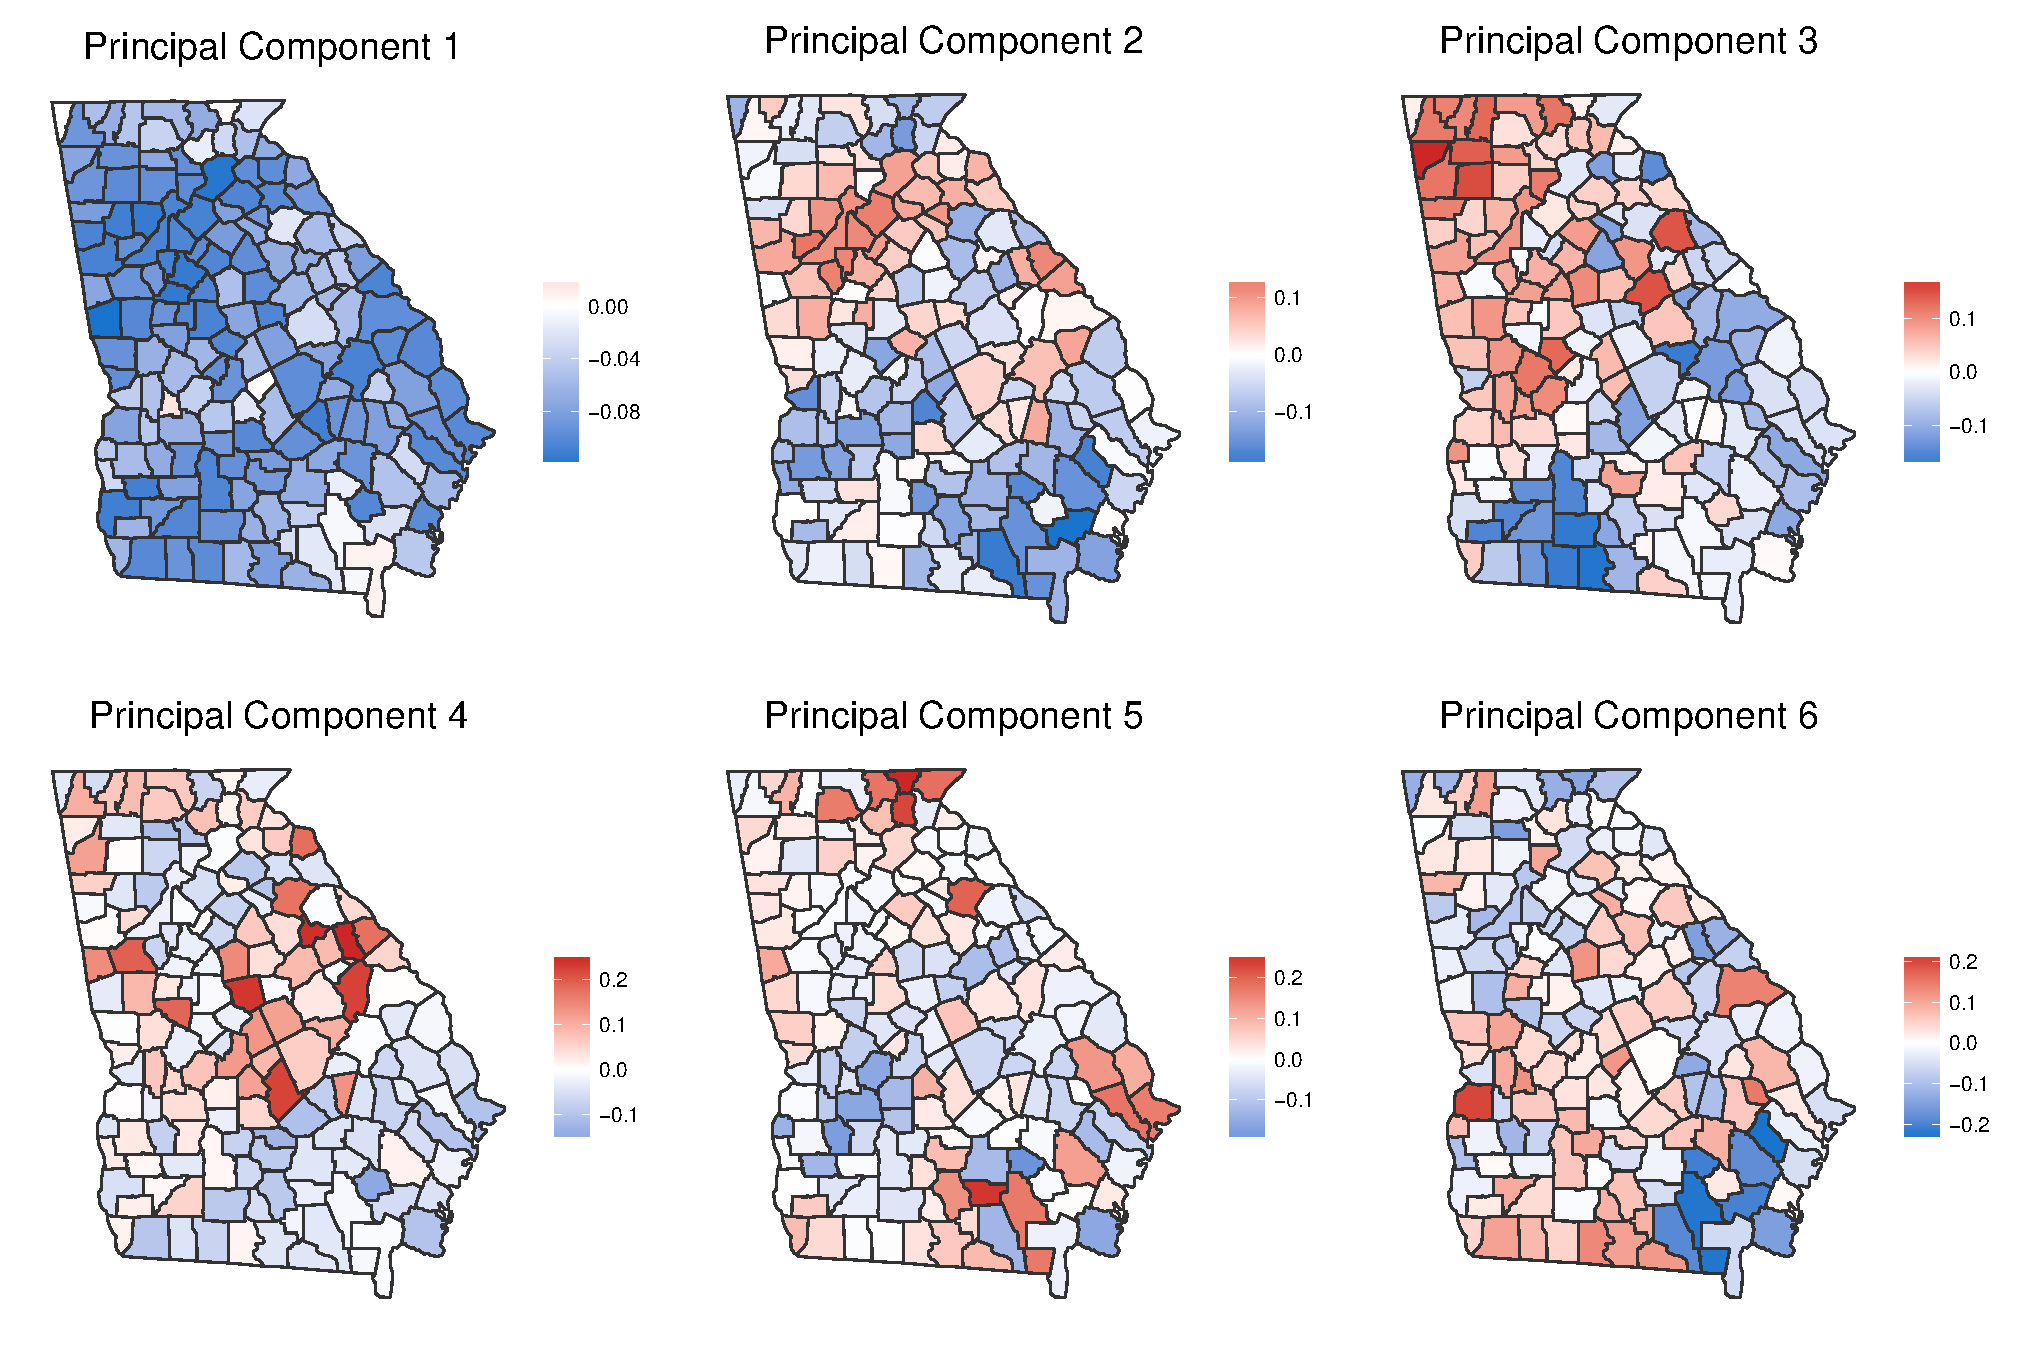
\includegraphics[width=0.9\textwidth]{fire-eig-panel}
	\end{center}
\end{frame}

\begin{frame}{Precipitation: PCs}
	\begin{center}
		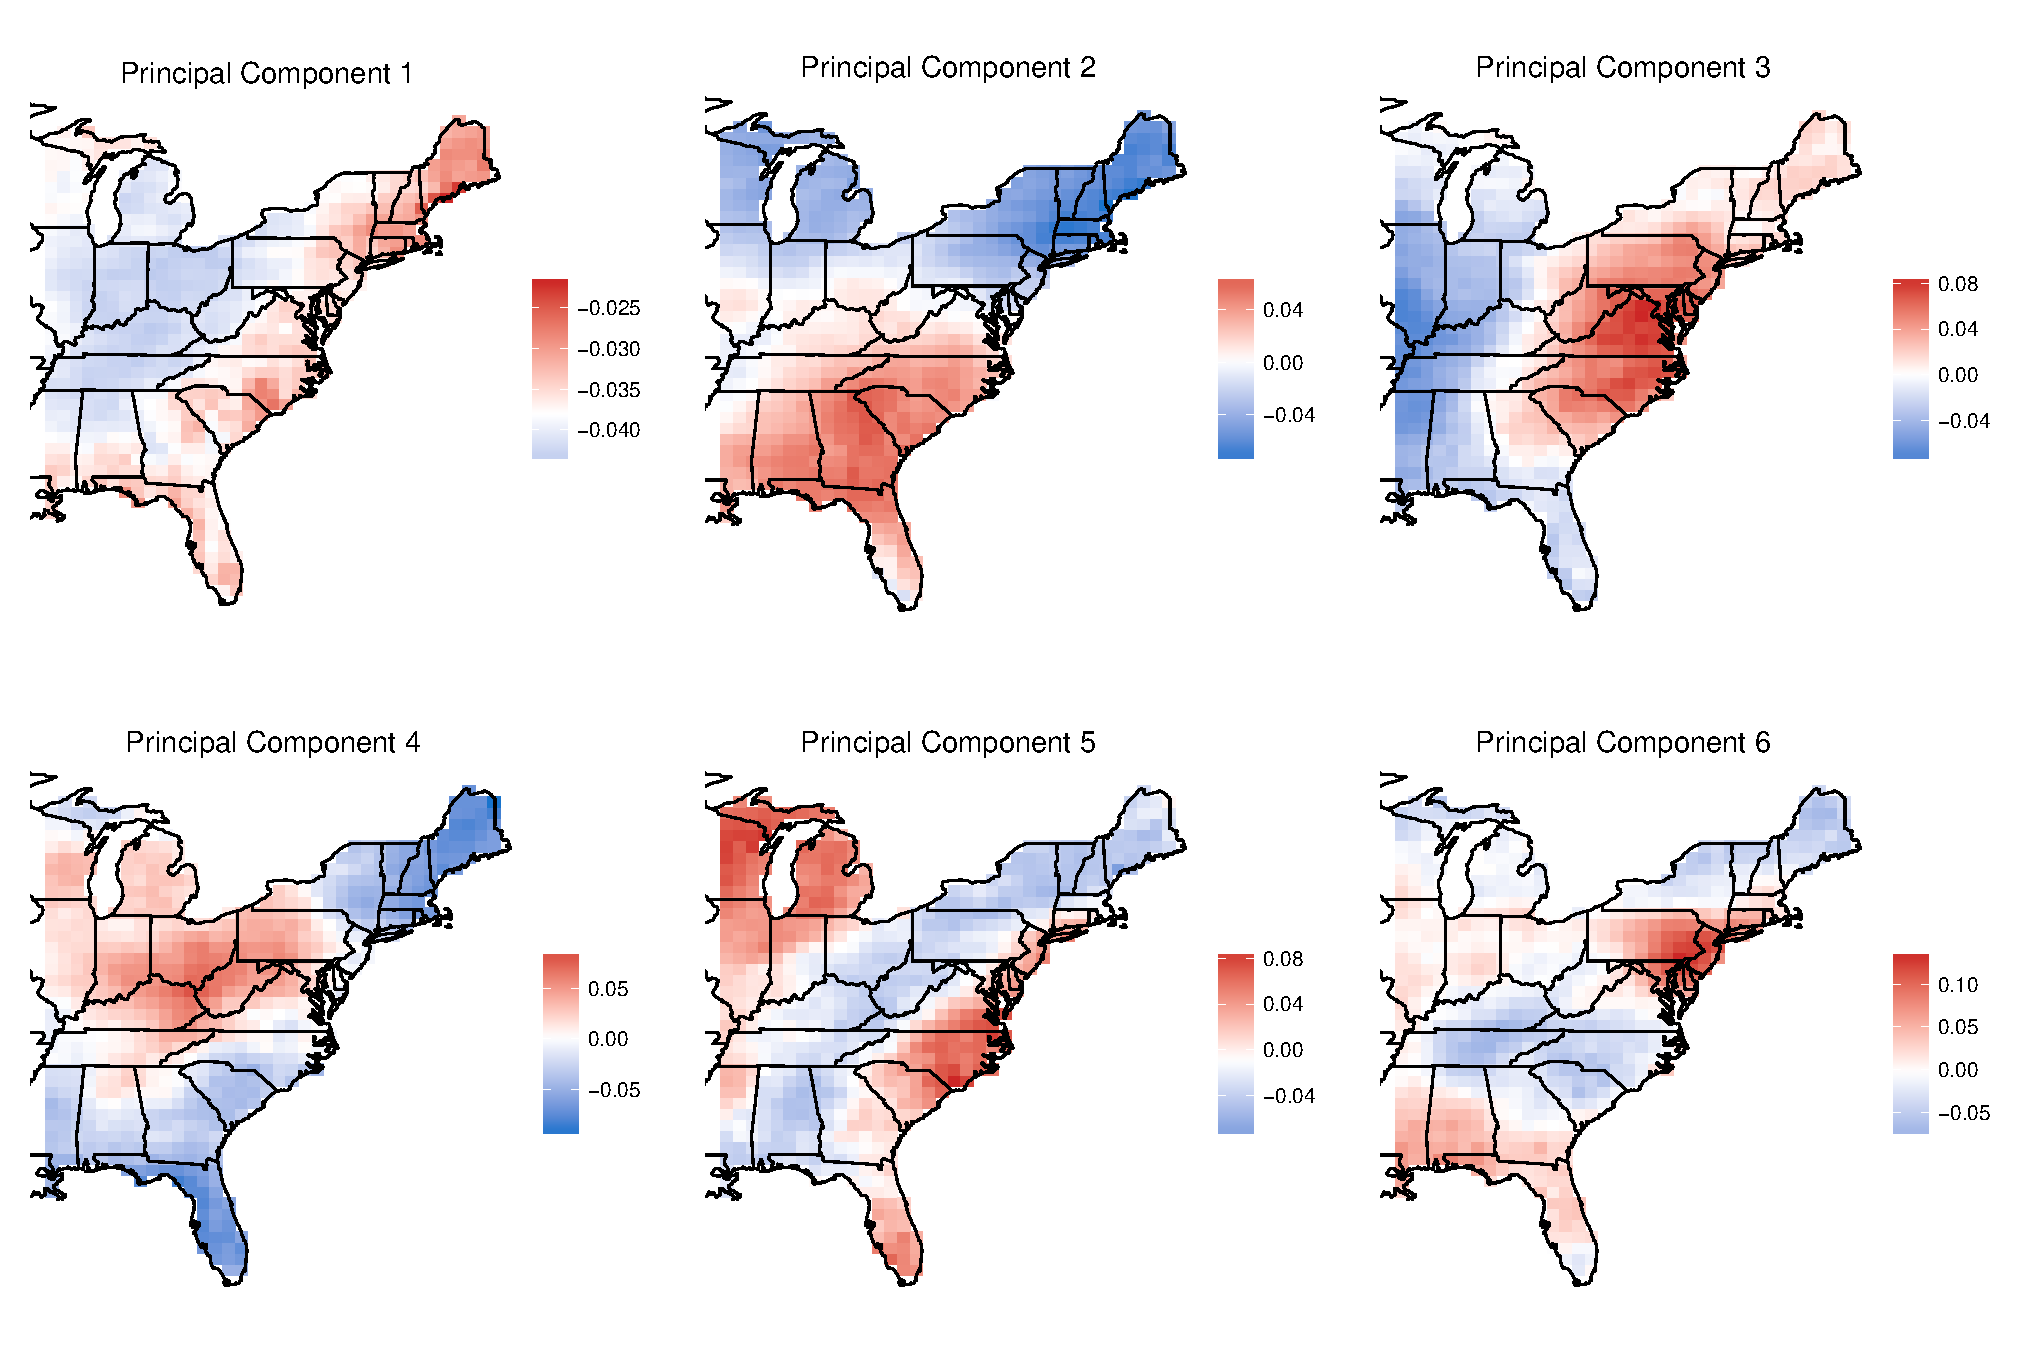
\includegraphics[width=0.9\textwidth]{precip-eig-panel}
	\end{center}
\end{frame}

%\begin{frame}[allowframebreaks]{References}
%  \begin{itemize} \setlength{\itemsep}{1em}
%    \item Balkema, A. A. and de Haan, L. (1974). Residual life time at great age, {\it Annals of Probability}, {\bf 2}, 792--804.
%    \item de Carvalho, M. and Davison, A. C. (2014). Spectral density ratio models for multivariate extremes, {\it Journal of the American Statistical Association}, {\bf 109}, 764--776.
%    \item Coles, S. G., Heffernan, J., and Tawn, J. A. (1999). Dependence measures for extreme value analysis, {\it Extremes}, {\bf 2}, 339--365.
%    \item Coles S. G. and Tawn, J. A. (1991). Modelling extreme multivariate events. {\it Journal of the Royal Statistical Society: Series B (Methodological)}, {\bf 53}, 337--392.
%    \item Demarta, S. and McNeil, A. J. (2007). The $t$ copula and related copulas. {\it International Statistical Review}, {\bf 73}, 111--129.
%    \item Falk. M., H\"{u}sler, J., and Reiss, R. D. (2010). {\it Laws of Small Numbers: Extremes and Rare Events}. Springer Basel.
%    \item Kim, H.-M., Mallik, B. K., and Holmes, C. C. (2005). Analyzing nonstationary spatial data using piecewise Gaussian processes. {\it Journal of the American Statistical Association}, {\bf 100}, 653--668.
%    \item Gnedenko, B. (1943). Sur la distribution limite du terme maximum d'une s\'{e}rie al\'{e}atoire. {\it Annals of Mathematics}, {\bf 44}, 423--453.
%    \item Gneiting, T. and Raftery, A. (2007). Strictly proper scoring rules, prediction, and estimation. {\it Journal of the American Statistical Association}, {\bf 102}, 359--378.
%    \item Gumbel, E. J. (1960). Multivariate extremal distributions. {\it Bulletin de l'Institut International de Statistique}, {\bf 37}, 471--475
%    \item Huser, R. and Davison, A. C. (2014). Space-time modelling of extreme events. {\it Journal of the Royal Statistical Society: Series B (Statistical Methodology)}, {\bf 76}, 439--461.
%    \item Padoan, S. A. (2011). Multivariate extreme models based on underlying skew-$t$ and skew-normal distributions. {\it Journal of Multivariate Analysis}, {\bf 102}, 977--991.
%    \item Reich, B. J. and Shaby, B. A. (2012). A hierarchical max-stable spatial model for extreme precipitation. {\it Annals of Applied Statistics}, {\bf 6}, 1430--1451.
%    \item Smith R. L. (1990). Max-stable processes and spatial extremes, unpublished manuscript.
%    \item Tawn, J. A. (1990). Modelling multivariate extreme value distributions. {\it Biometrika}, {\bf 77}, 245--253.
%    \item Zhang, H. and El-Shaarawi, A. (2010). On spatial skew-Gaussian processes and applications. {\it Environmetrics}, {\bf 21}, 33--47.
%  \end{itemize}
%\end{frame}

\end{document}